% Options for packages loaded elsewhere
\PassOptionsToPackage{unicode}{hyperref}
\PassOptionsToPackage{hyphens}{url}
\PassOptionsToPackage{dvipsnames,svgnames,x11names}{xcolor}
%
\documentclass[
  letterpaper,
  DIV=11,
  numbers=noendperiod]{scrreprt}

\usepackage{amsmath,amssymb}
\usepackage{iftex}
\ifPDFTeX
  \usepackage[T1]{fontenc}
  \usepackage[utf8]{inputenc}
  \usepackage{textcomp} % provide euro and other symbols
\else % if luatex or xetex
  \usepackage{unicode-math}
  \defaultfontfeatures{Scale=MatchLowercase}
  \defaultfontfeatures[\rmfamily]{Ligatures=TeX,Scale=1}
\fi
\usepackage{lmodern}
\ifPDFTeX\else  
    % xetex/luatex font selection
\fi
% Use upquote if available, for straight quotes in verbatim environments
\IfFileExists{upquote.sty}{\usepackage{upquote}}{}
\IfFileExists{microtype.sty}{% use microtype if available
  \usepackage[]{microtype}
  \UseMicrotypeSet[protrusion]{basicmath} % disable protrusion for tt fonts
}{}
\makeatletter
\@ifundefined{KOMAClassName}{% if non-KOMA class
  \IfFileExists{parskip.sty}{%
    \usepackage{parskip}
  }{% else
    \setlength{\parindent}{0pt}
    \setlength{\parskip}{6pt plus 2pt minus 1pt}}
}{% if KOMA class
  \KOMAoptions{parskip=half}}
\makeatother
\usepackage{xcolor}
\setlength{\emergencystretch}{3em} % prevent overfull lines
\setcounter{secnumdepth}{5}
% Make \paragraph and \subparagraph free-standing
\ifx\paragraph\undefined\else
  \let\oldparagraph\paragraph
  \renewcommand{\paragraph}[1]{\oldparagraph{#1}\mbox{}}
\fi
\ifx\subparagraph\undefined\else
  \let\oldsubparagraph\subparagraph
  \renewcommand{\subparagraph}[1]{\oldsubparagraph{#1}\mbox{}}
\fi

\usepackage{color}
\usepackage{fancyvrb}
\newcommand{\VerbBar}{|}
\newcommand{\VERB}{\Verb[commandchars=\\\{\}]}
\DefineVerbatimEnvironment{Highlighting}{Verbatim}{commandchars=\\\{\}}
% Add ',fontsize=\small' for more characters per line
\usepackage{framed}
\definecolor{shadecolor}{RGB}{241,243,245}
\newenvironment{Shaded}{\begin{snugshade}}{\end{snugshade}}
\newcommand{\AlertTok}[1]{\textcolor[rgb]{0.68,0.00,0.00}{#1}}
\newcommand{\AnnotationTok}[1]{\textcolor[rgb]{0.37,0.37,0.37}{#1}}
\newcommand{\AttributeTok}[1]{\textcolor[rgb]{0.40,0.45,0.13}{#1}}
\newcommand{\BaseNTok}[1]{\textcolor[rgb]{0.68,0.00,0.00}{#1}}
\newcommand{\BuiltInTok}[1]{\textcolor[rgb]{0.00,0.23,0.31}{#1}}
\newcommand{\CharTok}[1]{\textcolor[rgb]{0.13,0.47,0.30}{#1}}
\newcommand{\CommentTok}[1]{\textcolor[rgb]{0.37,0.37,0.37}{#1}}
\newcommand{\CommentVarTok}[1]{\textcolor[rgb]{0.37,0.37,0.37}{\textit{#1}}}
\newcommand{\ConstantTok}[1]{\textcolor[rgb]{0.56,0.35,0.01}{#1}}
\newcommand{\ControlFlowTok}[1]{\textcolor[rgb]{0.00,0.23,0.31}{#1}}
\newcommand{\DataTypeTok}[1]{\textcolor[rgb]{0.68,0.00,0.00}{#1}}
\newcommand{\DecValTok}[1]{\textcolor[rgb]{0.68,0.00,0.00}{#1}}
\newcommand{\DocumentationTok}[1]{\textcolor[rgb]{0.37,0.37,0.37}{\textit{#1}}}
\newcommand{\ErrorTok}[1]{\textcolor[rgb]{0.68,0.00,0.00}{#1}}
\newcommand{\ExtensionTok}[1]{\textcolor[rgb]{0.00,0.23,0.31}{#1}}
\newcommand{\FloatTok}[1]{\textcolor[rgb]{0.68,0.00,0.00}{#1}}
\newcommand{\FunctionTok}[1]{\textcolor[rgb]{0.28,0.35,0.67}{#1}}
\newcommand{\ImportTok}[1]{\textcolor[rgb]{0.00,0.46,0.62}{#1}}
\newcommand{\InformationTok}[1]{\textcolor[rgb]{0.37,0.37,0.37}{#1}}
\newcommand{\KeywordTok}[1]{\textcolor[rgb]{0.00,0.23,0.31}{#1}}
\newcommand{\NormalTok}[1]{\textcolor[rgb]{0.00,0.23,0.31}{#1}}
\newcommand{\OperatorTok}[1]{\textcolor[rgb]{0.37,0.37,0.37}{#1}}
\newcommand{\OtherTok}[1]{\textcolor[rgb]{0.00,0.23,0.31}{#1}}
\newcommand{\PreprocessorTok}[1]{\textcolor[rgb]{0.68,0.00,0.00}{#1}}
\newcommand{\RegionMarkerTok}[1]{\textcolor[rgb]{0.00,0.23,0.31}{#1}}
\newcommand{\SpecialCharTok}[1]{\textcolor[rgb]{0.37,0.37,0.37}{#1}}
\newcommand{\SpecialStringTok}[1]{\textcolor[rgb]{0.13,0.47,0.30}{#1}}
\newcommand{\StringTok}[1]{\textcolor[rgb]{0.13,0.47,0.30}{#1}}
\newcommand{\VariableTok}[1]{\textcolor[rgb]{0.07,0.07,0.07}{#1}}
\newcommand{\VerbatimStringTok}[1]{\textcolor[rgb]{0.13,0.47,0.30}{#1}}
\newcommand{\WarningTok}[1]{\textcolor[rgb]{0.37,0.37,0.37}{\textit{#1}}}

\providecommand{\tightlist}{%
  \setlength{\itemsep}{0pt}\setlength{\parskip}{0pt}}\usepackage{longtable,booktabs,array}
\usepackage{calc} % for calculating minipage widths
% Correct order of tables after \paragraph or \subparagraph
\usepackage{etoolbox}
\makeatletter
\patchcmd\longtable{\par}{\if@noskipsec\mbox{}\fi\par}{}{}
\makeatother
% Allow footnotes in longtable head/foot
\IfFileExists{footnotehyper.sty}{\usepackage{footnotehyper}}{\usepackage{footnote}}
\makesavenoteenv{longtable}
\usepackage{graphicx}
\makeatletter
\def\maxwidth{\ifdim\Gin@nat@width>\linewidth\linewidth\else\Gin@nat@width\fi}
\def\maxheight{\ifdim\Gin@nat@height>\textheight\textheight\else\Gin@nat@height\fi}
\makeatother
% Scale images if necessary, so that they will not overflow the page
% margins by default, and it is still possible to overwrite the defaults
% using explicit options in \includegraphics[width, height, ...]{}
\setkeys{Gin}{width=\maxwidth,height=\maxheight,keepaspectratio}
% Set default figure placement to htbp
\makeatletter
\def\fps@figure{htbp}
\makeatother

\KOMAoption{captions}{tableheading}
\makeatletter
\@ifpackageloaded{bookmark}{}{\usepackage{bookmark}}
\makeatother
\makeatletter
\@ifpackageloaded{caption}{}{\usepackage{caption}}
\AtBeginDocument{%
\ifdefined\contentsname
  \renewcommand*\contentsname{Table of contents}
\else
  \newcommand\contentsname{Table of contents}
\fi
\ifdefined\listfigurename
  \renewcommand*\listfigurename{List of Figures}
\else
  \newcommand\listfigurename{List of Figures}
\fi
\ifdefined\listtablename
  \renewcommand*\listtablename{List of Tables}
\else
  \newcommand\listtablename{List of Tables}
\fi
\ifdefined\figurename
  \renewcommand*\figurename{Figure}
\else
  \newcommand\figurename{Figure}
\fi
\ifdefined\tablename
  \renewcommand*\tablename{Table}
\else
  \newcommand\tablename{Table}
\fi
}
\@ifpackageloaded{float}{}{\usepackage{float}}
\floatstyle{ruled}
\@ifundefined{c@chapter}{\newfloat{codelisting}{h}{lop}}{\newfloat{codelisting}{h}{lop}[chapter]}
\floatname{codelisting}{Listing}
\newcommand*\listoflistings{\listof{codelisting}{List of Listings}}
\makeatother
\makeatletter
\makeatother
\makeatletter
\@ifpackageloaded{caption}{}{\usepackage{caption}}
\@ifpackageloaded{subcaption}{}{\usepackage{subcaption}}
\makeatother
\ifLuaTeX
  \usepackage{selnolig}  % disable illegal ligatures
\fi
\usepackage{bookmark}

\IfFileExists{xurl.sty}{\usepackage{xurl}}{} % add URL line breaks if available
\urlstyle{same} % disable monospaced font for URLs
\hypersetup{
  pdftitle={Simulación Matemática de Yacimientos},
  pdfauthor={Luis Miguel de la Cruz Salas},
  colorlinks=true,
  linkcolor={blue},
  filecolor={Maroon},
  citecolor={Blue},
  urlcolor={Blue},
  pdfcreator={LaTeX via pandoc}}

\title{Simulación Matemática de Yacimientos}
\author{Luis Miguel de la Cruz Salas}
\date{2023-01-12}

\begin{document}
\maketitle

\renewcommand*\contentsname{Table of contents}
{
\hypersetup{linkcolor=}
\setcounter{tocdepth}{2}
\tableofcontents
}
\bookmarksetup{startatroot}

\chapter*{Introducción}\label{introducciuxf3n}
\addcontentsline{toc}{chapter}{Introducción}

\markboth{Introducción}{Introducción}

Cuadernos interactivos para la asignatura de Simulación Matemática de
Yacimientos.

Los Jupyter Notebooks de este curso se pueden obtener en
\url{https://github.com/repomacti/macti/notebooks/}.

\bookmarksetup{startatroot}

\chapter{Sistemas de ecuaciones lineales:
introducción}\label{sistemas-de-ecuaciones-lineales-introducciuxf3n}

\textbf{Objetivo general} - Plantear y resolver un problema en términos
de la solución de un sistema de ecuaciones lineales.

\textbf{Objetivos particulares} - Entender como plantear un problema en
términos de un sistema de ecuaciones lineales. - Usar funciones de la
biblioteca \texttt{numpy} para resolver el problema. - Comparar varios
métodos para la solución de problemas más complejos.

MACTI NOTES by {Luis Miguel de la Cruz Salas} is licensed under CC
BY-NC-SA 4.0

\textbf{Trabajo realizado con el apoyo del Programa UNAM-DGAPA-PAPIME
PE101922}

\#\# Planes de telefonía móvil.

Dos compañías de telefonía compiten por ganar clientes. En la tabla que
sigue se muestra el costo de la renta y el costo por Megabyte (MB) de
datos de cada compañía.

\begin{longtable}[]{@{}ccc@{}}
\toprule\noalign{}
& Renta mensual & Costo por MB \\
\midrule\noalign{}
\endhead
\bottomrule\noalign{}
\endlastfoot
Compañía A & \(200\) & \(0.10\) \\
Compañía B & \(20\) & \(0.30\) \\
\end{longtable}

\textbf{¿Cómo podríamos decidir cuál de estas companías conviene
contratar?}

\#\#\# Modelo matemático - Observamos en la tabla anterior que la
compañía A tiene un precio fijo de 200 pesos mensuales que es 10 veces
mayor al precio que cobra la compañía B (20 pesos). - Por otro lado, la
compañía B cobra 0.30 pesos por cada MB, que es 3 veces mayor al precio
por MB de la compañía A. - El precio final mensual de cada compañía
depende básicamente de cuantos MB se usen.

Podemos escribir la forma en que cambia el precio de cada compañía en
función de los MB usados:

\$

\begin{array}{ccc}
P_A & = & 0.10 x + 200 \tag{1}\\
P_B & = & 0.30 x + 20
\end{array}

\$

donde \(x\) representa el número de MB usados durante un mes.

\subsection{Ejercicio 1. Gráfica de
rectas.}\label{ejercicio-1.-gruxe1fica-de-rectas.}

En el código siguiente complete las fórmulas para cada compañía de
acuerdo con las ecuaciones dadas en (1) y posteriormente ejecute el
código para obtener una gráfica de cómo cambia el precio en función de
los MB utilizados.

\begin{Shaded}
\begin{Highlighting}[]
\CommentTok{\# Importación de las bibliotecas numpy y matplotlib}
\ImportTok{import}\NormalTok{ numpy }\ImportTok{as}\NormalTok{ np}
\ImportTok{import}\NormalTok{ matplotlib.pyplot }\ImportTok{as}\NormalTok{ plt}
\ImportTok{import}\NormalTok{ sys, macti.visual}

\ImportTok{from}\NormalTok{ macti.evaluation }\ImportTok{import} \OperatorTok{*}
\end{Highlighting}
\end{Shaded}

\begin{Shaded}
\begin{Highlighting}[]
\NormalTok{quizz }\OperatorTok{=}\NormalTok{ Quizz(}\StringTok{\textquotesingle{}06\textquotesingle{}}\NormalTok{, }\StringTok{\textquotesingle{}notebooks\textquotesingle{}}\NormalTok{, }\StringTok{\textquotesingle{}local\textquotesingle{}}\NormalTok{)}
\end{Highlighting}
\end{Shaded}

Fórmulas a implementar: \$

\begin{array}{ccc}
P_A & = & 0.10 x + 200\\
P_B & = & 0.30 x + 20
\end{array}

\$

\begin{Shaded}
\begin{Highlighting}[]
\CommentTok{\# Megabytes desde 0 hasta 1500 (1.5 GB) en pasos de 10.}
\NormalTok{x }\OperatorTok{=}\NormalTok{ np.linspace(}\DecValTok{0}\NormalTok{,}\DecValTok{1500}\NormalTok{,}\DecValTok{10}\NormalTok{)}

\CommentTok{\# Fórmulas de cada compañía}
\CommentTok{\# PA = ...}
\CommentTok{\# PB = ...}
\CommentTok{\#}
\CommentTok{\#\#\# }\RegionMarkerTok{BEGIN}\CommentTok{ SOLUTION}
\NormalTok{PA }\OperatorTok{=} \FloatTok{0.10} \OperatorTok{*}\NormalTok{ x }\OperatorTok{+} \DecValTok{200}
\NormalTok{PB }\OperatorTok{=} \FloatTok{0.30} \OperatorTok{*}\NormalTok{ x }\OperatorTok{+} \DecValTok{20}

\NormalTok{file\_answer }\OperatorTok{=}\NormalTok{ FileAnswer()}
\NormalTok{file\_answer.write(}\StringTok{\textquotesingle{}1\textquotesingle{}}\NormalTok{, PA, }\StringTok{\textquotesingle{}Checa la fórmula para PA\textquotesingle{}}\NormalTok{)}
\NormalTok{file\_answer.write(}\StringTok{\textquotesingle{}2\textquotesingle{}}\NormalTok{, PB, }\StringTok{\textquotesingle{}Checa la fórmula para PB\textquotesingle{}}\NormalTok{)}
\CommentTok{\#\#\# }\RegionMarkerTok{END}\CommentTok{ SOLUTION}

\BuiltInTok{print}\NormalTok{(}\StringTok{\textquotesingle{}PA = }\SpecialCharTok{\{\}}\StringTok{\textquotesingle{}}\NormalTok{.}\BuiltInTok{format}\NormalTok{(PA))}
\BuiltInTok{print}\NormalTok{(}\StringTok{\textquotesingle{}Pb = }\SpecialCharTok{\{\}}\StringTok{\textquotesingle{}}\NormalTok{.}\BuiltInTok{format}\NormalTok{(PB))}
\end{Highlighting}
\end{Shaded}

\begin{verbatim}
El directorio :/home/jovyan/macti_notes/notebooks/.ans/SMM/ ya existe
Respuestas y retroalimentación almacenadas.
PA = [200.         216.66666667 233.33333333 250.         266.66666667
 283.33333333 300.         316.66666667 333.33333333 350.        ]
Pb = [ 20.  70. 120. 170. 220. 270. 320. 370. 420. 470.]
\end{verbatim}

\begin{Shaded}
\begin{Highlighting}[]
\NormalTok{quizz.eval\_numeric(}\StringTok{\textquotesingle{}1\textquotesingle{}}\NormalTok{, PA)}
\end{Highlighting}
\end{Shaded}

\begin{verbatim}
----------------------------------------
1 | Tu resultado es correcto.
----------------------------------------
\end{verbatim}

\begin{Shaded}
\begin{Highlighting}[]
\NormalTok{quizz.eval\_numeric(}\StringTok{\textquotesingle{}2\textquotesingle{}}\NormalTok{, PB)}
\end{Highlighting}
\end{Shaded}

\begin{verbatim}
----------------------------------------
2 | Tu resultado es correcto.
----------------------------------------
\end{verbatim}

\begin{Shaded}
\begin{Highlighting}[]
\CommentTok{\# Gráfica de ambos casos}
\NormalTok{plt.plot(x, PA, label }\OperatorTok{=} \StringTok{\textquotesingle{}Compañía A\textquotesingle{}}\NormalTok{)}
\NormalTok{plt.plot(x, PB, label }\OperatorTok{=} \StringTok{\textquotesingle{}Compañía B\textquotesingle{}}\NormalTok{)}

\CommentTok{\# Decoración de la gráfica}
\NormalTok{plt.xlabel(}\StringTok{\textquotesingle{}MB\textquotesingle{}}\NormalTok{)}
\NormalTok{plt.ylabel(}\StringTok{\textquotesingle{}Precio final\textquotesingle{}}\NormalTok{)}
\NormalTok{plt.legend()}
\NormalTok{plt.grid()}
\NormalTok{plt.show()}
\end{Highlighting}
\end{Shaded}

\includegraphics{01_Sol_Sist_Lineales_Intro_files/figure-pdf/cell-7-output-1.png}

\textbf{¿Qué observamos en la figura anterior?}

Para decidir cuál de los dos compañías elegir, debemos saber cuantos MB
gastamos al mes. En la figura se ve que al principio, con pocos MB
usados conviene contratar a la compañía B. Pero después, si hacemos uso
intenso de nuestras redes sociales, el consumo de MB aumenta y como
consecuencia el precio de la compañía A es más barato.

\textbf{¿Será posible determinar con precisión el punto de cruce de las
rectas?}

\#\#\# Sistema de ecuaciones lineales.

Las ecuaciones \((1)\) tienen la forma típica de una recta:
\(y = m x + b\)

Para la compañía A tenemos que \(m = 0.10\) y \(b = 200\), mientras que
para la compañía B tenemos \(m = 0.35\) y \(b = 20\), entonces
escribimos:

\[
\begin{array}{ccc}
y & = & 0.10 x + 200 \\
y & = & 0.35 x + 20
\end{array}
\]

Ahora, es posible escribir las ecuaciones de las líneas rectas en forma
de un sistema de ecuaciones lineales como sigue:

\[
\left[
\begin{array}{cc}
0.10 & -1 \\
0.35 & -1
\end{array} \right]
\left[
\begin{array}{c}
x \\
y
\end{array} \right] =
\left[
\begin{array}{c}
-200 \\ 
-20
\end{array} \right] \tag{2}
\]

\textbf{¿Puede verificar que el sistema (2) es correcto?}

Si resolvemos el sistema (2) entonces será posible conocer de manera
precisa el cruce de las rectas.

\subsection{Ejercicio 2. Solución del sistema
lineal.}\label{ejercicio-2.-soluciuxf3n-del-sistema-lineal.}

\begin{enumerate}
\def\labelenumi{\arabic{enumi}.}
\tightlist
\item
  En el siguiente código, complete los datos de la matriz \texttt{A} y
  el vector \texttt{b} de acuerdo con el sistema (2).
\end{enumerate}

\begin{Shaded}
\begin{Highlighting}[]
\CommentTok{\# Definimos la matriz A y el vector b}
\CommentTok{\# A = np.array([[],[]])}
\CommentTok{\# B = np.array([[]])}
\CommentTok{\#}
\CommentTok{\#\#\# }\RegionMarkerTok{BEGIN}\CommentTok{ SOLUTION}
\NormalTok{A }\OperatorTok{=}\NormalTok{ np.array([[}\FloatTok{0.10}\NormalTok{, }\OperatorTok{{-}}\FloatTok{1.}\NormalTok{],[}\FloatTok{0.30}\NormalTok{,}\OperatorTok{{-}}\FloatTok{1.}\NormalTok{]] )}
\NormalTok{b }\OperatorTok{=}\NormalTok{ np.array([[}\OperatorTok{{-}}\FloatTok{200.0}\NormalTok{,}\OperatorTok{{-}}\FloatTok{20.0}\NormalTok{]])}

\NormalTok{file\_answer.write(}\StringTok{\textquotesingle{}3\textquotesingle{}}\NormalTok{, A, }\StringTok{\textquotesingle{}Checa los elementos de la matriz A\textquotesingle{}}\NormalTok{)}
\NormalTok{file\_answer.write(}\StringTok{\textquotesingle{}4\textquotesingle{}}\NormalTok{, b, }\StringTok{\textquotesingle{}Checa los elementos del vector b\textquotesingle{}}\NormalTok{)}
\CommentTok{\#\#\# }\RegionMarkerTok{END}\CommentTok{ SOLUTION}

\BuiltInTok{print}\NormalTok{(}\StringTok{"Matriz A : }\CharTok{\textbackslash{}n}\StringTok{"}\NormalTok{,A)}
\BuiltInTok{print}\NormalTok{(}\StringTok{"Vector b : }\CharTok{\textbackslash{}n}\StringTok{"}\NormalTok{, b)}
\end{Highlighting}
\end{Shaded}

\begin{verbatim}
El directorio :/home/jovyan/macti_notes/notebooks/.ans/SMM/ ya existe
Respuestas y retroalimentación almacenadas.
Matriz A : 
 [[ 0.1 -1. ]
 [ 0.3 -1. ]]
Vector b : 
 [[-200.  -20.]]
\end{verbatim}

\begin{Shaded}
\begin{Highlighting}[]
\NormalTok{quizz.eval\_numeric(}\StringTok{\textquotesingle{}3\textquotesingle{}}\NormalTok{, A)}
\end{Highlighting}
\end{Shaded}

\begin{verbatim}
----------------------------------------
3 | Tu resultado es correcto.
----------------------------------------
\end{verbatim}

\begin{Shaded}
\begin{Highlighting}[]
\NormalTok{quizz.eval\_numeric(}\StringTok{\textquotesingle{}4\textquotesingle{}}\NormalTok{, b)}
\end{Highlighting}
\end{Shaded}

\begin{verbatim}
----------------------------------------
4 | Tu resultado es correcto.
----------------------------------------
\end{verbatim}

\begin{enumerate}
\def\labelenumi{\arabic{enumi}.}
\setcounter{enumi}{1}
\tightlist
\item
  Investigue como usar la función numpy.linalg.solve() para resolver el
  sistema de ecuaciones. Resuelva el sistema y guarde la solución en el
  vector \texttt{xsol}.
\end{enumerate}

\begin{Shaded}
\begin{Highlighting}[]
\CommentTok{\# Resolvemos el sistema de ecuaciones lineal}
\CommentTok{\# xsol = np.linalg.solve( ... )}
\CommentTok{\#}
\CommentTok{\#\#\# }\RegionMarkerTok{BEGIN}\CommentTok{ SOLUTION}
\NormalTok{xsol }\OperatorTok{=}\NormalTok{ np.linalg.solve(A,b.T) }

\NormalTok{file\_answer.write(}\StringTok{\textquotesingle{}5\textquotesingle{}}\NormalTok{, xsol, }\StringTok{\textquotesingle{}Verifica que usaste correctamente la función np.linalg.solve()\textquotesingle{}}\NormalTok{)}
\CommentTok{\#\#\# }\RegionMarkerTok{END}\CommentTok{ SOLUTION}

\BuiltInTok{print}\NormalTok{(}\StringTok{"Solución del sistema: }\CharTok{\textbackslash{}n}\StringTok{"}\NormalTok{, xsol)}
\end{Highlighting}
\end{Shaded}

\begin{verbatim}
El directorio :/home/jovyan/macti_notes/notebooks/.ans/SMM/ ya existe
Respuestas y retroalimentación almacenadas.
Solución del sistema: 
 [[900.]
 [290.]]
\end{verbatim}

\begin{Shaded}
\begin{Highlighting}[]
\NormalTok{quizz.eval\_numeric(}\StringTok{\textquotesingle{}5\textquotesingle{}}\NormalTok{, xsol)}
\end{Highlighting}
\end{Shaded}

\begin{verbatim}
----------------------------------------
5 | Tu resultado es correcto.
----------------------------------------
\end{verbatim}

\begin{Shaded}
\begin{Highlighting}[]
\CommentTok{\# Dot product}
\CommentTok{\# rhs = np.dot( ... )}
\CommentTok{\#}
\CommentTok{\#\#\# }\RegionMarkerTok{BEGIN}\CommentTok{ SOLUTION}
\NormalTok{rhs }\OperatorTok{=}\NormalTok{ np.dot(A, xsol)}

\NormalTok{file\_answer.write(}\StringTok{\textquotesingle{}6\textquotesingle{}}\NormalTok{, rhs, }\StringTok{\textquotesingle{}Checa que la representación de cada número sea la correcta.\textquotesingle{}}\NormalTok{)}
\NormalTok{file\_answer.to\_file(}\StringTok{\textquotesingle{}06\textquotesingle{}}\NormalTok{)}
\CommentTok{\#\#\# }\RegionMarkerTok{END}\CommentTok{ SOLUTION}

\BuiltInTok{print}\NormalTok{(rhs)}
\end{Highlighting}
\end{Shaded}

\begin{verbatim}
El directorio :/home/jovyan/macti_notes/notebooks/.ans/SMM/ ya existe
Respuestas y retroalimentación almacenadas.
[[-200.]
 [ -20.]]
\end{verbatim}

\begin{Shaded}
\begin{Highlighting}[]
\NormalTok{quizz.eval\_numeric(}\StringTok{\textquotesingle{}6\textquotesingle{}}\NormalTok{, rhs)}
\end{Highlighting}
\end{Shaded}

\begin{verbatim}
----------------------------------------
6 | Tu resultado es correcto.
----------------------------------------
\end{verbatim}

Si todo se hizo correctamente, el siguiente código debe graficar las
rectas de las dos compañías y en el punto donde se cruzan

\begin{Shaded}
\begin{Highlighting}[]
\CommentTok{\# Gráfica de las líneas de cada compañía}
\NormalTok{plt.plot(x, PA, lw}\OperatorTok{=}\DecValTok{3}\NormalTok{,label }\OperatorTok{=} \StringTok{\textquotesingle{}A\textquotesingle{}}\NormalTok{)}
\NormalTok{plt.plot(x, PB, lw}\OperatorTok{=}\DecValTok{3}\NormalTok{,label }\OperatorTok{=} \StringTok{\textquotesingle{}B\textquotesingle{}}\NormalTok{)}

\CommentTok{\# Punto de cruce de las líneas rectas}
\NormalTok{plt.scatter(xsol[}\DecValTok{0}\NormalTok{], xsol[}\DecValTok{1}\NormalTok{], fc }\OperatorTok{=} \StringTok{\textquotesingle{}C3\textquotesingle{}}\NormalTok{, ec }\OperatorTok{=}\StringTok{\textquotesingle{}k\textquotesingle{}}\NormalTok{, s }\OperatorTok{=} \DecValTok{100}\NormalTok{, alpha}\OperatorTok{=}\FloatTok{0.85}\NormalTok{, zorder}\OperatorTok{=}\DecValTok{5}\NormalTok{, label}\OperatorTok{=}\StringTok{\textquotesingle{}Solución\textquotesingle{}}\NormalTok{)}

\CommentTok{\# Decoración de la gráfica}
\NormalTok{plt.xlabel(}\StringTok{\textquotesingle{}MB\textquotesingle{}}\NormalTok{)}
\NormalTok{plt.ylabel(}\StringTok{\textquotesingle{}Precio final\textquotesingle{}}\NormalTok{)}
\NormalTok{plt.title(}\StringTok{\textquotesingle{}Cruce de las rectas: (}\SpecialCharTok{\{:4.0f\}}\StringTok{ MB, }\SpecialCharTok{\{:4.0f\}}\StringTok{ pesos)\textquotesingle{}}\NormalTok{.}\BuiltInTok{format}\NormalTok{(xsol[}\DecValTok{0}\NormalTok{][}\DecValTok{0}\NormalTok{], xsol[}\DecValTok{1}\NormalTok{][}\DecValTok{0}\NormalTok{]))}
\NormalTok{plt.vlines(xsol[}\DecValTok{0}\NormalTok{][}\DecValTok{0}\NormalTok{], }\DecValTok{0}\NormalTok{, xsol[}\DecValTok{1}\NormalTok{][}\DecValTok{0}\NormalTok{], ls}\OperatorTok{=}\StringTok{\textquotesingle{}{-}{-}\textquotesingle{}}\NormalTok{, lw}\OperatorTok{=}\FloatTok{1.0}\NormalTok{, color}\OperatorTok{=}\StringTok{\textquotesingle{}gray\textquotesingle{}}\NormalTok{)}
\NormalTok{plt.hlines(xsol[}\DecValTok{1}\NormalTok{][}\DecValTok{0}\NormalTok{], }\DecValTok{0}\NormalTok{, xsol[}\DecValTok{0}\NormalTok{][}\DecValTok{0}\NormalTok{], ls}\OperatorTok{=}\StringTok{\textquotesingle{}{-}{-}\textquotesingle{}}\NormalTok{, lw}\OperatorTok{=}\FloatTok{1.0}\NormalTok{, color}\OperatorTok{=}\StringTok{\textquotesingle{}gray\textquotesingle{}}\NormalTok{)}

\NormalTok{plt.grid(}\VariableTok{True}\NormalTok{)}
\NormalTok{plt.legend()}
\NormalTok{plt.show()}
\end{Highlighting}
\end{Shaded}

\includegraphics{01_Sol_Sist_Lineales_Intro_files/figure-pdf/cell-15-output-1.png}

\bookmarksetup{startatroot}

\chapter{Métodos iterativos para la solución de sistemas de ecuaciones
lineales}\label{muxe9todos-iterativos-para-la-soluciuxf3n-de-sistemas-de-ecuaciones-lineales}

\textbf{Objetivo.}

Describir e implementar los algoritmos de Jacobi, Gauss-Seidel y SOR
para la solución de sistemas de ecuaciones lineales.

MACTI-Algebra\_Lineal\_01 by Luis M. de la Cruz is licensed under
Attribution-ShareAlike 4.0 International

Trabajo realizado con el apoyo del Programa UNAM-DGAPA-PAPIME PE101922

\begin{Shaded}
\begin{Highlighting}[]
\ImportTok{import}\NormalTok{ numpy }\ImportTok{as}\NormalTok{ np}
\ImportTok{import}\NormalTok{ ipywidgets }\ImportTok{as}\NormalTok{ widgets}
\ImportTok{import}\NormalTok{ macti.visual }\ImportTok{as}\NormalTok{ mvis}
\end{Highlighting}
\end{Shaded}

\bookmarksetup{startatroot}

\chapter{Cruce de dos rectas.}\label{cruce-de-dos-rectas.}

Las siguientes dos rectas se cruzan en algún punto.

\[
\begin{array}{ccc}
3x + 2y & = &2 \\
2x + 6y & = &-8
\end{array}
\]

Las ecuaciones de las rectas se pueden escribir como:

\[
\begin{array}{ccc}
\dfrac{3}{2}x + y & = & 1 \\
\dfrac{2}{6}x + y & = & -\dfrac{8}{6}
\end{array} \Longrightarrow
\begin{array}{ccc}
y = m_1 x + b_1 \\
y = m_2 x + b_2
\end{array} \text{ donde }
\begin{array}{ccc}
m_1 = -\dfrac{3}{2} & b_1 = 1 \\
m_2 = -\dfrac{2}{6} & b_2 = -\dfrac{8}{6}
\end{array}
\]

Ahora realizaremos la gráfica de las rectas:

\section{Definición y gráfica de las
rectas}\label{definiciuxf3n-y-gruxe1fica-de-las-rectas}

\section{\texorpdfstring{\textbf{Ejercicio
1.}}{Ejercicio 1.}}\label{ejercicio-1.}

En la siguiente celda se define el domino \(x\) para las líneas rectas,
los parámetros para construir la línea recta 1 y su construcción. De la
misma manera define los parámetros y construye la recta 2. Si todo lo
hiciste correctamente, la celda de graficación mostrará las gráficas de
las líneas rectas.

\begin{Shaded}
\begin{Highlighting}[]
\ImportTok{from}\NormalTok{ macti.evaluation }\ImportTok{import}\NormalTok{ FileAnswer, Quizz}
\CommentTok{\#file\_anser = FileAnswer()}
\CommentTok{\#quizz = Quizz()}
\end{Highlighting}
\end{Shaded}

\begin{Shaded}
\begin{Highlighting}[]
\CommentTok{\# Dominio}
\NormalTok{x }\OperatorTok{=}\NormalTok{ np.linspace(}\OperatorTok{{-}}\DecValTok{3}\NormalTok{,}\DecValTok{6}\NormalTok{,}\DecValTok{10}\NormalTok{)}

\CommentTok{\# Línea recta 1}
\NormalTok{m1 }\OperatorTok{=} \OperatorTok{{-}}\DecValTok{3}\OperatorTok{/}\DecValTok{2}
\NormalTok{b1 }\OperatorTok{=} \DecValTok{1}
\NormalTok{y1 }\OperatorTok{=}\NormalTok{ m1 }\OperatorTok{*}\NormalTok{ x }\OperatorTok{+}\NormalTok{ b1}

\CommentTok{\# Línea recta 2}
\CommentTok{\# m2 = ...}
\CommentTok{\# b2 = ...}
\CommentTok{\# y2 = ...}

\CommentTok{\#\#\# }\RegionMarkerTok{BEGIN}\CommentTok{ SOLUTION}
\NormalTok{m2 }\OperatorTok{=} \OperatorTok{{-}}\DecValTok{2}\OperatorTok{/}\DecValTok{6}
\NormalTok{b2 }\OperatorTok{=} \OperatorTok{{-}}\DecValTok{8}\OperatorTok{/}\DecValTok{6}
\NormalTok{y2 }\OperatorTok{=}\NormalTok{ m2 }\OperatorTok{*}\NormalTok{ x }\OperatorTok{+}\NormalTok{ b2}

\CommentTok{\#file\_answer(\textquotesingle{}1\textquotesingle{}, m2, \textquotesingle{}m2 incorrecta revisa el valor del parámetro.\textquotesingle{})}
\CommentTok{\#file\_answer(\textquotesingle{}2\textquotesingle{}, b2, \textquotesingle{}b2 incorrecta revisa el valor del parámetro.\textquotesingle{})}
\CommentTok{\#file\_answer(\textquotesingle{}3\textquotesingle{}, y2, \textquotesingle{}y2 no está definida correctamente.\textquotesingle{})}
\CommentTok{\#\#\# }\RegionMarkerTok{END}\CommentTok{ SOLUTION}
\end{Highlighting}
\end{Shaded}

\begin{Shaded}
\begin{Highlighting}[]
\CommentTok{\#quizz.eval\_numeric(\textquotesingle{}1\textquotesingle{}, m2)}
\CommentTok{\#quizz.eval\_numeric(\textquotesingle{}2\textquotesingle{}, b2)}
\CommentTok{\#quizz.eval\_numeric(\textquotesingle{}3\textquotesingle{}, y2)}
\end{Highlighting}
\end{Shaded}

\textbf{Gráfica de las líneas rectas.}

\begin{Shaded}
\begin{Highlighting}[]
\NormalTok{v }\OperatorTok{=}\NormalTok{ mvis.Plotter(}\DecValTok{1}\NormalTok{,}\DecValTok{1}\NormalTok{,[}\BuiltInTok{dict}\NormalTok{(aspect}\OperatorTok{=}\StringTok{\textquotesingle{}equal\textquotesingle{}}\NormalTok{)],title}\OperatorTok{=}\StringTok{\textquotesingle{}Cruce de rectas\textquotesingle{}}\NormalTok{) }
\NormalTok{v.set\_coordsys(}\DecValTok{1}\NormalTok{)}
\NormalTok{v.plot(}\DecValTok{1}\NormalTok{, x, y1, lw }\OperatorTok{=} \DecValTok{3}\NormalTok{, c }\OperatorTok{=} \StringTok{\textquotesingle{}seagreen\textquotesingle{}}\NormalTok{, label }\OperatorTok{=} \StringTok{\textquotesingle{}$3x+2y=2$\textquotesingle{}}\NormalTok{) }\CommentTok{\# Línea recta 1}
\NormalTok{v.plot(}\DecValTok{1}\NormalTok{, x, y2, lw }\OperatorTok{=} \DecValTok{3}\NormalTok{, c }\OperatorTok{=} \StringTok{\textquotesingle{}mediumorchid\textquotesingle{}}\NormalTok{,label }\OperatorTok{=} \StringTok{\textquotesingle{}$2x+6y={-}8$\textquotesingle{}}\NormalTok{) }\CommentTok{\# Línea recta 2}
\NormalTok{v.legend(ncol }\OperatorTok{=} \DecValTok{1}\NormalTok{, frameon}\OperatorTok{=}\VariableTok{True}\NormalTok{, loc}\OperatorTok{=}\StringTok{\textquotesingle{}best\textquotesingle{}}\NormalTok{, bbox\_to\_anchor}\OperatorTok{=}\NormalTok{(}\FloatTok{1.75}\NormalTok{, }\FloatTok{1.05}\NormalTok{))}
\NormalTok{v.grid()}
\NormalTok{v.show()}
\end{Highlighting}
\end{Shaded}

\includegraphics{02_Sol_Sis_Lin_Iter_1_files/figure-pdf/cell-6-output-1.png}

\section{Sistemas lineales.}\label{sistemas-lineales.}

Las ecuaciones de las rectas se pueden escribir en forma de un sistema
lineal:

\[
\left[
\begin{array}{cc}
3 & 2 \\
2 & 6
\end{array} \right]
\left[
\begin{array}{c}
x_{0} \\
x_{1}
\end{array} \right] =
\left[
\begin{array}{c}
2 \\ 
-8
\end{array} \right]
\tag{1}
\]

Podemos calcular el cruce de las rectas resolviendo el sistema lineal:

\section{\texorpdfstring{\textbf{Ejemplo
1.}}{Ejemplo 1.}}\label{ejemplo-1.}

Definir el sistema lineal y resolverlo. Posteriomente graficar las
rectas y el punto solución.

El sistema lineal se puede resolver directamente con la función
\texttt{np.linalg.solve()} como sigue:

\begin{Shaded}
\begin{Highlighting}[]
\NormalTok{A }\OperatorTok{=}\NormalTok{ np.array([[}\DecValTok{3}\NormalTok{, }\DecValTok{2}\NormalTok{],[}\DecValTok{2}\NormalTok{,}\DecValTok{6}\NormalTok{]] )}
\NormalTok{b }\OperatorTok{=}\NormalTok{ np.array([[}\DecValTok{2}\NormalTok{,}\OperatorTok{{-}}\DecValTok{8}\NormalTok{]])}
\BuiltInTok{print}\NormalTok{(}\StringTok{"Matriz A : }\CharTok{\textbackslash{}n}\StringTok{"}\NormalTok{,A)}
\BuiltInTok{print}\NormalTok{(}\StringTok{"Vector b : }\CharTok{\textbackslash{}n}\StringTok{"}\NormalTok{, b)}

\NormalTok{sol }\OperatorTok{=}\NormalTok{ np.linalg.solve(A,b[}\DecValTok{0}\NormalTok{]) }\CommentTok{\# Función del módulo linalg para resolver el sistema}
\BuiltInTok{print}\NormalTok{(}\StringTok{"Solución del sistema: "}\NormalTok{, sol)}
\end{Highlighting}
\end{Shaded}

\begin{verbatim}
Matriz A : 
 [[3 2]
 [2 6]]
Vector b : 
 [[ 2 -8]]
Solución del sistema:  [ 2. -2.]
\end{verbatim}

\textbf{Gráfica de las líneas rectas y el punto de cruce (solución).}

\begin{Shaded}
\begin{Highlighting}[]
\NormalTok{v }\OperatorTok{=}\NormalTok{ mvis.Plotter(}\DecValTok{1}\NormalTok{,}\DecValTok{1}\NormalTok{,[}\BuiltInTok{dict}\NormalTok{(aspect}\OperatorTok{=}\StringTok{\textquotesingle{}equal\textquotesingle{}}\NormalTok{)],title}\OperatorTok{=}\StringTok{\textquotesingle{}Cruce de rectas\textquotesingle{}}\NormalTok{) }
\NormalTok{v.set\_coordsys(}\DecValTok{1}\NormalTok{)}
\NormalTok{v.plot(}\DecValTok{1}\NormalTok{, x, y1, lw }\OperatorTok{=} \DecValTok{3}\NormalTok{, c }\OperatorTok{=} \StringTok{\textquotesingle{}seagreen\textquotesingle{}}\NormalTok{, label }\OperatorTok{=} \StringTok{\textquotesingle{}$3x+2y=2$\textquotesingle{}}\NormalTok{) }\CommentTok{\# Línea recta 1}
\NormalTok{v.plot(}\DecValTok{1}\NormalTok{, x, y2, lw }\OperatorTok{=} \DecValTok{3}\NormalTok{, c }\OperatorTok{=} \StringTok{\textquotesingle{}mediumorchid\textquotesingle{}}\NormalTok{, label }\OperatorTok{=} \StringTok{\textquotesingle{}$2x+6y={-}8$\textquotesingle{}}\NormalTok{) }\CommentTok{\# Línea recta 2}
\NormalTok{v.scatter(}\DecValTok{1}\NormalTok{, sol[}\DecValTok{0}\NormalTok{], sol[}\DecValTok{1}\NormalTok{], fc}\OperatorTok{=}\StringTok{\textquotesingle{}sandybrown\textquotesingle{}}\NormalTok{, ec}\OperatorTok{=}\StringTok{\textquotesingle{}k\textquotesingle{}}\NormalTok{, s }\OperatorTok{=} \DecValTok{75}\NormalTok{, alpha}\OperatorTok{=}\FloatTok{0.75}\NormalTok{, zorder}\OperatorTok{=}\DecValTok{5}\NormalTok{, label}\OperatorTok{=}\StringTok{\textquotesingle{}Sol. final\textquotesingle{}}\NormalTok{) }\CommentTok{\# Solución}
\NormalTok{v.legend(ncol }\OperatorTok{=} \DecValTok{1}\NormalTok{, frameon}\OperatorTok{=}\VariableTok{True}\NormalTok{, loc}\OperatorTok{=}\StringTok{\textquotesingle{}best\textquotesingle{}}\NormalTok{, bbox\_to\_anchor}\OperatorTok{=}\NormalTok{(}\FloatTok{1.75}\NormalTok{, }\FloatTok{1.05}\NormalTok{))}
\NormalTok{v.grid()}
\NormalTok{v.show()}
\end{Highlighting}
\end{Shaded}

\includegraphics{02_Sol_Sis_Lin_Iter_1_files/figure-pdf/cell-8-output-1.png}

En general, un sistema de ecuaciones lineales de \(n \times n\) se
escribe como sigue:

\[
\begin{array}{ccccccc}
a_{11}x_1 & + & a_{12}x_2 & +  \dots  + & a_{1n}x_n & = & b_1 \\
a_{21}x_1 & + & a_{22}x_2 & +  \dots + & a_{2n}x_n & = & b_2 \\
\vdots & & \vdots &  & \vdots & & \vdots \\
a_{i1}x_1 & + & a_{i2}x_2 & +  \dots + & a_{in}x_n & = & b_i \\
\vdots & & \vdots &  & \vdots & & \vdots \\
a_{n1}x_1 & + & a_{n2}x_2 & + \dots + & a_{nn}x_n & = & b_n
\end{array}
\]

Es posible usar diferentes métodos para resolver este tipo de sistemas.
Veamos tres de ellos.

\bookmarksetup{startatroot}

\chapter{Método de Jacobi}\label{muxe9todo-de-jacobi}

\begin{itemize}
\item
  En este método, de la primera ecuación se despeja \(x_1\); de la
  segunda ecuación se despeja \(x_2\); y a sí sucesivamente, de tal
  manera que obtenemos: \[
  \begin{eqnarray*}
    x_1 & = &\left( b_1 - (a_{12}x_2 +  \dots  + a_{1n}x_n) \right) / a_{11}  \\
    x_2 & = &\left( b_2 - (a_{21}x_1 +  \dots  + a_{2n}x_n) \right) / a_{22} \\
    \vdots & & \vdots \\
    x_i & = &\left( b_i - (a_{i1}x_1 +  \dots  + a_{in}x_n) \right) / a_{ii} \\
    \vdots & & \vdots \\
    x_n & = &\left( b_n - (a_{n1}x_1 +  \dots  + a_{nn-1}x_{n-1}) \right) / a_{nn}
  \end{eqnarray*}
  \]
\item
  Suponemos ahora que tenemos una solución inicial aproximada
  \(\mathbf{x}^0 = [x_1^0, \dots, x_n^0]\). Usando esta solución
  inicial, es posible hacer una nueva aproximación para obtener
  \(\mathbf{x}^1 = [x_1^1, \dots, x_n^1]\) como sigue:
\end{itemize}

\[
\begin{eqnarray*}
    x_1^1 & = &\left( b_1 - (a_{12}x_2^0 +  \dots  + a_{1n}x_n^0) \right) / a_{11}  \\
    x_2^1 & = &\left( b_2 - (a_{21}x_1^0 +  \dots  + a_{2n}x_n^0) \right) / a_{22} \\
    \vdots & & \vdots \\
    x_i^1 & = &\left( b_i - (a_{i1}x_1^0 +  \dots  + a_{in}x_n^0) \right) / a_{ii} \\
    \vdots & & \vdots \\
    x_n^1 & = &\left( b_n - (a_{n1}x_1^0 +  \dots  + a_{nn-1}x_{n-1}^0) \right) / a_{nn}
\end{eqnarray*}
\]

\begin{itemize}
\tightlist
\item
  En general para \(i = 1, \dots, n\) y \(k = 1, 2, \dots\) tenemos:
\end{itemize}

\[
x_i^k = \frac{1}{a_{i,i}} \left(b_i -  \sum_{j \neq i} a_{i,j} x_j^{k-1} \right)
\]

\begin{itemize}
\tightlist
\item
  En términos de matrices, la \textbf{iteración de Jacobi} se escribe:
  \[
  \mathbf{x}^k = -\mathbf{D}^{-1} \mathbf{B}\mathbf{x}^{k-1} + \mathbf{D}^{-1} \mathbf{b}
  \]
\end{itemize}

donde \(\mathbf{D}\) es la matriz diagonal y
\(\mathbf{B} = \mathbf{A} - \mathbf{D}\).

\begin{itemize}
\tightlist
\item
  El cálculo de cada componente \(x_i^k\) es independiente de las otras
  componentes, por lo que este método se conoce también como de
  \emph{desplazamientos simultáneos}.
\end{itemize}

\section{Algoritmo Jacobi.}\label{algoritmo-jacobi.}

En general, podemos definir el siguiente algoritmo para el método de
Jacobi.

Observa que en este algoritmo hay un ciclo \texttt{while} el cual
termina cuando el error es menor o igual que una tolerancia \texttt{tol}
o se ha alcanzado un número máximo de iteraciones \texttt{kmax}. En la
línea \textbf{11} se calcula el error, que en términos matemáticos se
define como \(error = || \mathbf{x}^k - \mathbf{x}||\) donde
\(\mathbf{x}^k\) es la aproximación de la iteración \(k\)-ésima y
\(\mathbf{x}\) es la solución exacta. En muchas ocasiones no se tiene
acceso a la solución exacta por lo que se compara con la solución de la
iteración anterior, es decir
\(error = || \mathbf{x}^k - \mathbf{x}^{k-1}||\). En los ejemplos que
siguen si tenemos la solución exacta, por lo que haremos la comparación
con ella.

\section{Implementación.}\label{implementaciuxf3n.}

\begin{Shaded}
\begin{Highlighting}[]
\KeywordTok{def}\NormalTok{ jacobi(A,b,tol,kmax,xi, yi):}
\NormalTok{    N }\OperatorTok{=} \BuiltInTok{len}\NormalTok{(b[}\DecValTok{0}\NormalTok{])}
\NormalTok{    xnew }\OperatorTok{=}\NormalTok{ np.zeros(N)}
\NormalTok{    xold }\OperatorTok{=}\NormalTok{ np.zeros(N)}
\NormalTok{    x }\OperatorTok{=}\NormalTok{ np.array([}\DecValTok{2}\NormalTok{, }\OperatorTok{{-}}\DecValTok{2}\NormalTok{]) }\CommentTok{\# Solución exacta}
    
    \CommentTok{\# Solución inicial}
\NormalTok{    xold[}\DecValTok{0}\NormalTok{] }\OperatorTok{=}\NormalTok{ xi}
\NormalTok{    xold[}\DecValTok{1}\NormalTok{] }\OperatorTok{=}\NormalTok{ yi}
    
\NormalTok{    xs }\OperatorTok{=}\NormalTok{ [xi]}
\NormalTok{    ys }\OperatorTok{=}\NormalTok{ [yi]}
    
\NormalTok{    e }\OperatorTok{=} \DecValTok{10}
\NormalTok{    error }\OperatorTok{=}\NormalTok{ [] }
    
\NormalTok{    k }\OperatorTok{=} \DecValTok{0}
    \BuiltInTok{print}\NormalTok{(}\StringTok{\textquotesingle{}}\SpecialCharTok{\{:\^{}2\}}\StringTok{ }\SpecialCharTok{\{:\^{}10\}}\StringTok{ }\SpecialCharTok{\{:\^{}12\}}\StringTok{ }\SpecialCharTok{\{:\^{}12\}}\StringTok{\textquotesingle{}}\NormalTok{.}\BuiltInTok{format}\NormalTok{(}\StringTok{\textquotesingle{} i \textquotesingle{}}\NormalTok{, }\StringTok{\textquotesingle{}Error\textquotesingle{}}\NormalTok{, }\StringTok{\textquotesingle{}x0\textquotesingle{}}\NormalTok{, }\StringTok{\textquotesingle{}x1\textquotesingle{}}\NormalTok{))}
    \ControlFlowTok{while}\NormalTok{(e }\OperatorTok{\textgreater{}}\NormalTok{ tol }\KeywordTok{and}\NormalTok{ k }\OperatorTok{\textless{}}\NormalTok{ kmax) :}
        \ControlFlowTok{for}\NormalTok{ i }\KeywordTok{in} \BuiltInTok{range}\NormalTok{(}\DecValTok{0}\NormalTok{,N): }\CommentTok{\# se puede hacer en paralelo}
\NormalTok{            xnew[i] }\OperatorTok{=} \DecValTok{0}
            \ControlFlowTok{for}\NormalTok{ j }\KeywordTok{in} \BuiltInTok{range}\NormalTok{(}\DecValTok{0}\NormalTok{,i):}
\NormalTok{                xnew[i] }\OperatorTok{+=}\NormalTok{ A[i,j] }\OperatorTok{*}\NormalTok{ xold[j]}
            \ControlFlowTok{for}\NormalTok{ j }\KeywordTok{in} \BuiltInTok{range}\NormalTok{(i}\OperatorTok{+}\DecValTok{1}\NormalTok{,N):}
\NormalTok{                xnew[i] }\OperatorTok{+=}\NormalTok{ A[i,j] }\OperatorTok{*}\NormalTok{ xold[j]                }
\NormalTok{            xnew[i] }\OperatorTok{=}\NormalTok{ (b[}\DecValTok{0}\NormalTok{,i] }\OperatorTok{{-}}\NormalTok{ xnew[i]) }\OperatorTok{/}\NormalTok{ A[i,i]}
        
        \CommentTok{\# Almacenamos la solución actual}
\NormalTok{        xs.append(xnew[}\DecValTok{0}\NormalTok{])}
\NormalTok{        ys.append(xnew[}\DecValTok{1}\NormalTok{])}
        
\NormalTok{        e }\OperatorTok{=}\NormalTok{ np.linalg.norm(xnew}\OperatorTok{{-}}\NormalTok{x, }\DecValTok{2}\NormalTok{) }\CommentTok{\# Cálculo del error}
\NormalTok{        error.append(e)}
\NormalTok{        k }\OperatorTok{+=} \DecValTok{1}
\NormalTok{        xold[:] }\OperatorTok{=}\NormalTok{ xnew[:]}
        \BuiltInTok{print}\NormalTok{(}\StringTok{\textquotesingle{}}\SpecialCharTok{\{:2d\}}\StringTok{ }\SpecialCharTok{\{:10.9f\}}\StringTok{ (}\SpecialCharTok{\{:10.9f\}}\StringTok{, }\SpecialCharTok{\{:10.9f\}}\StringTok{)\textquotesingle{}}\NormalTok{.}\BuiltInTok{format}\NormalTok{(k, e, xnew[}\DecValTok{0}\NormalTok{], xnew[}\DecValTok{1}\NormalTok{]))}
    \ControlFlowTok{return}\NormalTok{ xnew, np.array(xs), np.array(ys), error, k}
\end{Highlighting}
\end{Shaded}

\section{\texorpdfstring{\textbf{Ejemplo 3. Aplicación del método de
Jacobi.}}{Ejemplo 3. Aplicación del método de Jacobi.}}\label{ejemplo-3.-aplicaciuxf3n-del-muxe9todo-de-jacobi.}

Haciendo uso de la función \texttt{jacobi} definida en la celda
anterior, aproxima la solución del sistema de ecuaciones (1). Utiliza la
solución inicial \texttt{(xi,\ yi)} = \((-2, 2)\), una tolerancia
\texttt{tol} = \(1 \times 10^{-5}\) y \texttt{kmax} = \(50\)
iteraciones.

\begin{Shaded}
\begin{Highlighting}[]
\CommentTok{\# Solución inicial}
\NormalTok{(xi, yi) }\OperatorTok{=}\NormalTok{ (}\OperatorTok{{-}}\DecValTok{2}\NormalTok{, }\DecValTok{2}\NormalTok{)}
\NormalTok{tol }\OperatorTok{=} \FloatTok{1e{-}5}
\NormalTok{kmax }\OperatorTok{=} \DecValTok{50}

\CommentTok{\# Ejecución del método de Jacobi}
\NormalTok{solJ, xs, ys, eJ, itJ }\OperatorTok{=}\NormalTok{ jacobi(A, b, tol, kmax, xi, yi)}
\end{Highlighting}
\end{Shaded}

\begin{verbatim}
 i    Error         x0           x1     
 1 2.981423970 (-0.666666667, -0.666666667)
 2 1.257078722 (1.111111111, -1.111111111)
 3 0.662538660 (1.407407407, -1.703703704)
 4 0.279350827 (1.802469136, -1.802469136)
 5 0.147230813 (1.868312757, -1.934156379)
 6 0.062077962 (1.956104252, -1.956104252)
 7 0.032717959 (1.970736168, -1.985368084)
 8 0.013795103 (1.990245389, -1.990245389)
 9 0.007270657 (1.993496926, -1.996748463)
10 0.003065578 (1.997832309, -1.997832309)
11 0.001615702 (1.998554873, -1.999277436)
12 0.000681240 (1.999518291, -1.999518291)
13 0.000359045 (1.999678861, -1.999839430)
14 0.000151387 (1.999892954, -1.999892954)
15 0.000079788 (1.999928636, -1.999964318)
16 0.000033641 (1.999976212, -1.999976212)
17 0.000017731 (1.999984141, -1.999992071)
18 0.000007476 (1.999994714, -1.999994714)
\end{verbatim}

Observa que la función \texttt{jacobi()} regresa 5 valores: *
\texttt{solJ} la solución obtenida, * \texttt{xs} y \texttt{ys}
componentes de las soluciones aproximadas en cada paso, * \texttt{eJ} el
error con respecto a la solución exacta e * \texttt{itJ} el número de
iteraciones realizadas.

A continuación graficamos como es que la solución se va aproximando con
este método.

\begin{Shaded}
\begin{Highlighting}[]
\NormalTok{v }\OperatorTok{=}\NormalTok{ mvis.Plotter(}\DecValTok{1}\NormalTok{,}\DecValTok{1}\NormalTok{,[}\BuiltInTok{dict}\NormalTok{(aspect}\OperatorTok{=}\StringTok{\textquotesingle{}equal\textquotesingle{}}\NormalTok{)],title}\OperatorTok{=}\StringTok{\textquotesingle{}Cruce de rectas\textquotesingle{}}\NormalTok{) }
\NormalTok{v.set\_coordsys(}\DecValTok{1}\NormalTok{)}
\NormalTok{v.plot(}\DecValTok{1}\NormalTok{, x, y1, lw }\OperatorTok{=} \DecValTok{3}\NormalTok{, c }\OperatorTok{=} \StringTok{\textquotesingle{}seagreen\textquotesingle{}}\NormalTok{, label }\OperatorTok{=} \StringTok{\textquotesingle{}$3x+2y=2$\textquotesingle{}}\NormalTok{) }\CommentTok{\# Línea recta 1}
\NormalTok{v.plot(}\DecValTok{1}\NormalTok{, x, y2, lw }\OperatorTok{=} \DecValTok{3}\NormalTok{, c }\OperatorTok{=} \StringTok{\textquotesingle{}mediumorchid\textquotesingle{}}\NormalTok{, label }\OperatorTok{=} \StringTok{\textquotesingle{}$2x+6y={-}8$\textquotesingle{}}\NormalTok{) }\CommentTok{\# Línea recta 2}
\NormalTok{v.scatter(}\DecValTok{1}\NormalTok{, sol[}\DecValTok{0}\NormalTok{], sol[}\DecValTok{1}\NormalTok{], fc}\OperatorTok{=}\StringTok{\textquotesingle{}sandybrown\textquotesingle{}}\NormalTok{, ec}\OperatorTok{=}\StringTok{\textquotesingle{}k\textquotesingle{}}\NormalTok{, s }\OperatorTok{=} \DecValTok{75}\NormalTok{, alpha}\OperatorTok{=}\FloatTok{0.75}\NormalTok{, zorder}\OperatorTok{=}\DecValTok{5}\NormalTok{, label}\OperatorTok{=}\StringTok{\textquotesingle{}Sol. final\textquotesingle{}}\NormalTok{) }\CommentTok{\# Solución}

\CommentTok{\# Graficamos los pasos}
\NormalTok{v.scatter(}\DecValTok{1}\NormalTok{, xs[}\DecValTok{0}\NormalTok{], ys[}\DecValTok{0}\NormalTok{], fc}\OperatorTok{=}\StringTok{\textquotesingle{}yellow\textquotesingle{}}\NormalTok{, ec}\OperatorTok{=}\StringTok{\textquotesingle{}k\textquotesingle{}}\NormalTok{, s }\OperatorTok{=} \DecValTok{75}\NormalTok{, alpha}\OperatorTok{=}\FloatTok{0.75}\NormalTok{, zorder}\OperatorTok{=}\DecValTok{8}\NormalTok{, label}\OperatorTok{=}\StringTok{\textquotesingle{}Sol. inicial\textquotesingle{}}\NormalTok{)}
\NormalTok{v.scatter(}\DecValTok{1}\NormalTok{, xs[}\DecValTok{1}\NormalTok{:], ys[}\DecValTok{1}\NormalTok{:], c}\OperatorTok{=}\StringTok{\textquotesingle{}navy\textquotesingle{}}\NormalTok{, s }\OperatorTok{=} \DecValTok{10}\NormalTok{, alpha}\OperatorTok{=}\FloatTok{0.5}\NormalTok{, zorder}\OperatorTok{=}\DecValTok{8}\NormalTok{)}
\NormalTok{v.plot(}\DecValTok{1}\NormalTok{, xs, ys, c}\OperatorTok{=}\StringTok{\textquotesingle{}grey\textquotesingle{}}\NormalTok{, ls }\OperatorTok{=} \StringTok{\textquotesingle{}{-}{-}\textquotesingle{}}\NormalTok{, lw}\OperatorTok{=}\FloatTok{1.0}\NormalTok{, zorder}\OperatorTok{=}\DecValTok{8}\NormalTok{, label}\OperatorTok{=}\StringTok{\textquotesingle{}Pasos de Jacobi\textquotesingle{}}\NormalTok{)}

\NormalTok{v.legend(ncol }\OperatorTok{=} \DecValTok{1}\NormalTok{, frameon}\OperatorTok{=}\VariableTok{True}\NormalTok{, loc}\OperatorTok{=}\StringTok{\textquotesingle{}best\textquotesingle{}}\NormalTok{, bbox\_to\_anchor}\OperatorTok{=}\NormalTok{(}\FloatTok{1.80}\NormalTok{, }\FloatTok{1.01}\NormalTok{))}
\NormalTok{v.grid()}
\NormalTok{v.show()}
\end{Highlighting}
\end{Shaded}

\includegraphics{02_Sol_Sis_Lin_Iter_1_files/figure-pdf/cell-11-output-1.png}

\section{Cálculo del error}\label{cuxe1lculo-del-error}

\begin{itemize}
\item
  Definimos \(e_i^k = x_i^k - x_i\) como la diferencia entre la
  \(i\)-ésima componente de la solución exacta y la \(i\)-ésima
  componente de la \(k\)-ésima iteración, de tal manera que
  \(\mathbf{e} = [e_1, \dots, e_n]^T\) es el vector error.
\item
  Aplicando una vez la iteración de Jacobi para \(x_i\) y \(x_i^{k+1}\)
  podemos escribir la diferencia como sigue:
\end{itemize}

\[
\begin{eqnarray*}
\left| e_i^{k+1} \right| & = &\left| x_i^{k+1} - x_i  \right| \\
\left| e_i^{k+1} \right| & = & \left|
\frac{1}{a_{i,i}} \left(b_i - \sum_{j \neq i} a_{i,j} x_j^{k} \right) -
\frac{1}{a_{i,i}} \left(b_i - \sum_{j \neq i} a_{i,j} x_j \right) \right| \\
\left| e_i^{k+1} \right| & = & \left| -\sum_{j \neq i} \frac{a_{i,j}}{a_{i,i}} (x_j^k - x_j)\right| \\
\left| e_i^{k+1} \right| & = & \left| -\sum_{j \neq i} \frac{a_{i,j}}{a_{i,i}} e_j^k \right| 
\le \sum_{j \neq i} \left| \frac{a_{i,j}}{a_{i,i}} \right| || \mathbf{e}^k ||_\infty, \qquad \forall i, k .
\end{eqnarray*}
\]

\begin{itemize}
\item
  En particular: \[
  \max_{1 \le i \le n} \left( \left| e_i^{k+1} \right| \right) =  || \mathbf{e}^{k+1} ||_\infty
   \le \sum_{j \neq i} \left| \frac{a_{i,j}}{a_{i,i}} \right| || \mathbf{e}^k ||_\infty
  \]
\item
  Definimos
  \(\displaystyle K = \max_{1 \le i \le n} \sum_{j \neq i} \left| \frac{a_{i,j}}{a_{i,i}} \right|\)
  entonces:
\end{itemize}

\[
\begin{eqnarray*}
|| \mathbf{e}^{k+1} ||_\infty & \le &  K || \mathbf{e}^{k} ||_\infty \le K \left( K || \mathbf{e}^{k-1} ||_\infty \right) \le
\dots \le K^k || \mathbf{e}^{1} ||_\infty \\
|| \mathbf{e}^{k+1} ||_\infty & \le &  K^k || \mathbf{e}^{1} ||_\infty
\end{eqnarray*}
\]

\begin{itemize}
\item
  Si \(K < 1\) entonces \(\mathbf{e}^{k} \rightarrow 0\) cuando
  \(k \rightarrow \infty\)
\item
  La condición \(K < 1\) implica: \[
  \sum_{j \neq i} |a_{i,j}| < |a_{i,i}|, \forall i
  \]
\end{itemize}

A continuación graficamos el error que se va obteniendo en cada paso del
método:

\begin{Shaded}
\begin{Highlighting}[]
\CommentTok{\# Lista con el número de las iteraciones}
\NormalTok{l\_itJ }\OperatorTok{=} \BuiltInTok{list}\NormalTok{(}\BuiltInTok{range}\NormalTok{(}\DecValTok{1}\NormalTok{,itJ}\OperatorTok{+}\DecValTok{1}\NormalTok{)) }

\CommentTok{\# Parámetros para los ejes}
\NormalTok{a\_p }\OperatorTok{=} \BuiltInTok{dict}\NormalTok{(yscale}\OperatorTok{=}\StringTok{\textquotesingle{}log\textquotesingle{}}\NormalTok{, xlabel}\OperatorTok{=}\StringTok{\textquotesingle{}Iteraciones\textquotesingle{}}\NormalTok{, xticks }\OperatorTok{=}\NormalTok{ l\_itJ)}

\CommentTok{\# Gráfica del error}
\NormalTok{v }\OperatorTok{=}\NormalTok{ mvis.Plotter(}\DecValTok{1}\NormalTok{,}\DecValTok{1}\NormalTok{,[a\_p]) }
\NormalTok{v.axes(}\DecValTok{1}\NormalTok{).set\_title(}\StringTok{\textquotesingle{}Error\textquotesingle{}}\NormalTok{, loc}\OperatorTok{=}\StringTok{\textquotesingle{}left\textquotesingle{}}\NormalTok{)}
\NormalTok{v.plot(}\DecValTok{1}\NormalTok{, l\_itJ, eJ, marker}\OperatorTok{=}\StringTok{\textquotesingle{}.\textquotesingle{}}\NormalTok{, label}\OperatorTok{=}\StringTok{\textquotesingle{}Jacobi\textquotesingle{}}\NormalTok{) }\CommentTok{\# Error eJ}
\NormalTok{v.legend()}
\NormalTok{v.grid()}
\end{Highlighting}
\end{Shaded}

\includegraphics{02_Sol_Sis_Lin_Iter_1_files/figure-pdf/cell-12-output-1.png}

\bookmarksetup{startatroot}

\chapter{Método de Gauss-Seidel}\label{muxe9todo-de-gauss-seidel}

\begin{itemize}
\item
  La principal diferencia con el método de Jacobi es que las ecuaciones
  se analizan en un orden determinado.
\item
  Por ejemplo, si realizamos el cálculo en orden ascendente y ya hemos
  evaluado \(x_1\) y \(x_2\), para evaluar \(x_3\) haríamos lo
  siguiente:\} \[
  \begin{eqnarray*}
  \underline{x_1^1} & = &\left( b_1 - (a_{12}x_2^0 + a_{13} x_3^0 + \dots  + a_{1n}x_n^0) \right) / a_{11}  \\
  \underline{x_2^1} & = &\left( b_2 - (a_{21}\underline{x_1^1} + a_{23}x_3^0 + \dots  + a_{2n}x_n^0) \right) / a_{22} \\
  x_3 & = &\left( b_3 - (a_{31}\underline{x_1^1} + a_{32}\underline{x_2^1} + \dots  + a_{3n}x_n^0)\right) / a_{22}
  \end{eqnarray*}
  \]
\item
  En general la fórmula del método es como sigue: \$\$ x\_i\^{}k =
  \frac{1}{a_{i,i}} \left(b\_i - \sum\emph{\{j \textless{} i\} a}\{i,j\}
  \underline{x_j^{k}}
\item
  \sum\emph{\{j \textgreater{} i\} a}\{i,j\} x\_j\^{}\{k-1\} \right)
  \$\$
\item
  Este algoritmo es serial dado que cada componente depende de que las
  componentes previas se hayan calculado (\emph{desplazamientos
  sucesivos}).
\item
  El valor de la nueva iteración \(\mathbf{x}^k\) depende del orden en
  que se examinan las componentes. Si se cambia el orden, el valor de
  \(\mathbf{x}^k\) cambia.
\end{itemize}

\section{Algoritmo Gauss-Seidel.}\label{algoritmo-gauss-seidel.}

En general, podemos definir el siguiente algoritmo para el método de
Gauss-Seidel.

Se aplican los mismo comentarios que para el algoritmo de Jacobi.

\section{Implementación.}\label{implementaciuxf3n.-1}

\begin{Shaded}
\begin{Highlighting}[]
\KeywordTok{def}\NormalTok{ gauss\_seidel(A,b,tol,kmax,xi,yi):}
\NormalTok{    N }\OperatorTok{=} \BuiltInTok{len}\NormalTok{(b[}\DecValTok{0}\NormalTok{])}
\NormalTok{    xnew }\OperatorTok{=}\NormalTok{ np.zeros(N)}
\NormalTok{    xold }\OperatorTok{=}\NormalTok{ np.zeros(N)}
\NormalTok{    x }\OperatorTok{=}\NormalTok{ np.array([}\DecValTok{2}\NormalTok{, }\OperatorTok{{-}}\DecValTok{2}\NormalTok{]) }\CommentTok{\# Solución exacta}

    \CommentTok{\# Solución inicial}
\NormalTok{    xold[}\DecValTok{0}\NormalTok{] }\OperatorTok{=}\NormalTok{ xi}
\NormalTok{    xold[}\DecValTok{1}\NormalTok{] }\OperatorTok{=}\NormalTok{ yi}

\NormalTok{    xs }\OperatorTok{=}\NormalTok{ [xi]}
\NormalTok{    ys }\OperatorTok{=}\NormalTok{ [yi]}
    
\NormalTok{    e }\OperatorTok{=} \DecValTok{10}
\NormalTok{    error }\OperatorTok{=}\NormalTok{ [] }
    
\NormalTok{    k }\OperatorTok{=} \DecValTok{0}
    \BuiltInTok{print}\NormalTok{(}\StringTok{\textquotesingle{}}\SpecialCharTok{\{:\^{}2\}}\StringTok{ }\SpecialCharTok{\{:\^{}10\}}\StringTok{ }\SpecialCharTok{\{:\^{}12\}}\StringTok{ }\SpecialCharTok{\{:\^{}12\}}\StringTok{\textquotesingle{}}\NormalTok{.}\BuiltInTok{format}\NormalTok{(}\StringTok{\textquotesingle{} i \textquotesingle{}}\NormalTok{, }\StringTok{\textquotesingle{}Error\textquotesingle{}}\NormalTok{, }\StringTok{\textquotesingle{}x0\textquotesingle{}}\NormalTok{, }\StringTok{\textquotesingle{}x1\textquotesingle{}}\NormalTok{))}
    \ControlFlowTok{while}\NormalTok{(e }\OperatorTok{\textgreater{}}\NormalTok{ tol }\KeywordTok{and}\NormalTok{ k }\OperatorTok{\textless{}}\NormalTok{ kmax) :}
        \ControlFlowTok{for}\NormalTok{ i }\KeywordTok{in} \BuiltInTok{range}\NormalTok{(}\DecValTok{0}\NormalTok{,N): }\CommentTok{\# se puede hacer en paralelo}
\NormalTok{            xnew[i] }\OperatorTok{=} \DecValTok{0}
            \ControlFlowTok{for}\NormalTok{ j }\KeywordTok{in} \BuiltInTok{range}\NormalTok{(}\DecValTok{0}\NormalTok{,i):}
\NormalTok{                xnew[i] }\OperatorTok{+=}\NormalTok{ A[i,j] }\OperatorTok{*}\NormalTok{ xnew[j]}
            \ControlFlowTok{for}\NormalTok{ j }\KeywordTok{in} \BuiltInTok{range}\NormalTok{(i}\OperatorTok{+}\DecValTok{1}\NormalTok{,N):}
\NormalTok{                xnew[i] }\OperatorTok{+=}\NormalTok{ A[i,j] }\OperatorTok{*}\NormalTok{ xold[j]                }
\NormalTok{            xnew[i] }\OperatorTok{=}\NormalTok{ (b[}\DecValTok{0}\NormalTok{,i] }\OperatorTok{{-}}\NormalTok{ xnew[i]) }\OperatorTok{/}\NormalTok{ A[i,i]}
            
        \CommentTok{\# Almacenamos la solución actual}
\NormalTok{        xs.append(xnew[}\DecValTok{0}\NormalTok{])}
\NormalTok{        ys.append(xnew[}\DecValTok{1}\NormalTok{])}

\NormalTok{        e }\OperatorTok{=}\NormalTok{ np.linalg.norm(xnew}\OperatorTok{{-}}\NormalTok{x,}\DecValTok{2}\NormalTok{) }\CommentTok{\# Cálculo del error}
\NormalTok{        error.append(e)}
\NormalTok{        k }\OperatorTok{+=} \DecValTok{1}
\NormalTok{        xold[:] }\OperatorTok{=}\NormalTok{ xnew[:]}
        \BuiltInTok{print}\NormalTok{(}\StringTok{\textquotesingle{}}\SpecialCharTok{\{:2d\}}\StringTok{ }\SpecialCharTok{\{:10.9f\}}\StringTok{ (}\SpecialCharTok{\{:10.9f\}}\StringTok{, }\SpecialCharTok{\{:10.9f\}}\StringTok{)\textquotesingle{}}\NormalTok{.}\BuiltInTok{format}\NormalTok{(k, e, xnew[}\DecValTok{0}\NormalTok{], xnew[}\DecValTok{1}\NormalTok{]))}
    \ControlFlowTok{return}\NormalTok{ xnew, np.array(xs), np.array(ys), error, k}
\end{Highlighting}
\end{Shaded}

\section{\texorpdfstring{\textbf{Ejercicio
2.}}{Ejercicio 2.}}\label{ejercicio-2.}

Haciendo uso de la función \texttt{gauss\_seidel()} definida en la celda
anterior, aproxima la solución del sistema de ecuaciones del Ejemplo 1.
Utiliza la solución inicial \texttt{(xi,\ yi)\ =} \((-2, 2)\), una
tolerancia \texttt{tol} = \(1 \times 10^{-5}\) y \texttt{kmax} = \(50\)
iteraciones. Utiliza las variables \texttt{solG}, \texttt{xs},
\texttt{ys}, \texttt{eG} e \texttt{itG} para almacenar la salida de la
función \texttt{gauss\_seidel()}. Posteriormente grafica las rectas y
cómo se va calculando la solución con este método (puedes usar el mismo
código que en el caso de Jacobi). Grafica también los errores para el
método de Jacobi y para el de Gauss-Seidel, deberías obtener una imagen
como la siguiente:

\textbf{Cálculo de la solución con Gauss-Seidel}

\begin{Shaded}
\begin{Highlighting}[]
\CommentTok{\# Solución inicial}
\CommentTok{\# xi, yi = }
\CommentTok{\# tol = }
\CommentTok{\# kmax = }

\CommentTok{\# Método de Gauss{-}Seidel}
\CommentTok{\# ...}

\CommentTok{\#\#\# }\RegionMarkerTok{BEGIN}\CommentTok{ SOLUTION}
\CommentTok{\# Solución inicial}
\NormalTok{xi, yi }\OperatorTok{=} \OperatorTok{{-}}\DecValTok{2}\NormalTok{, }\DecValTok{2}
\NormalTok{tol }\OperatorTok{=} \FloatTok{1e{-}5}
\NormalTok{kmax }\OperatorTok{=} \DecValTok{50}

\CommentTok{\# Método de Gauss{-}Seidel}
\NormalTok{solG, xs, ys, eG, itG }\OperatorTok{=}\NormalTok{ gauss\_seidel(A, b, tol, kmax, xi, yi)}

\CommentTok{\#file\_answer.write(\textquotesingle{}4\textquotesingle{}, solG, \textquotesingle{}solG es incorrecta: revisa la llamada y ejecución de la función gauss\_seidel() así como sus parámetros de entrada.\textquotesingle{})}
\CommentTok{\#file\_answer.write(\textquotesingle{}5\textquotesingle{}, eG[{-}1], \textquotesingle{}eG[{-}1] es incorrecto: revisa la llamada y ejecución de la función gauss\_seidel() así como sus parámetros de entrada.\textquotesingle{})}
\CommentTok{\#file\_answer.write(\textquotesingle{}6\textquotesingle{}, itG, \textquotesingle{}itG es incorrector: revisa la llamada y ejecución de la función gauss\_seidel() así como sus parámetros de entrada.\textquotesingle{})}

\CommentTok{\#\#\# }\RegionMarkerTok{END}\CommentTok{ SOLUTION}
\end{Highlighting}
\end{Shaded}

\begin{verbatim}
 i    Error         x0           x1     
 1 2.810913476 (-0.666666667, -1.111111111)
 2 0.624647439 (1.407407407, -1.802469136)
 3 0.138810542 (1.868312757, -1.956104252)
 4 0.030846787 (1.970736168, -1.990245389)
 5 0.006854842 (1.993496926, -1.997832309)
 6 0.001523298 (1.998554873, -1.999518291)
 7 0.000338511 (1.999678861, -1.999892954)
 8 0.000075225 (1.999928636, -1.999976212)
 9 0.000016717 (1.999984141, -1.999994714)
10 0.000003715 (1.999996476, -1.999998825)
\end{verbatim}

\begin{Shaded}
\begin{Highlighting}[]
\CommentTok{\#quizz.eval\_numeric(\textquotesingle{}4\textquotesingle{}, solG)}
\CommentTok{\#quizz.eval\_numeric(\textquotesingle{}5\textquotesingle{}, eG[{-}1])}
\CommentTok{\#quizz.eval\_numeric(\textquotesingle{}6\textquotesingle{}, itG)}
\end{Highlighting}
\end{Shaded}

\textbf{Gráfica de las rectas, la solución y los pasos realizados}

\begin{Shaded}
\begin{Highlighting}[]
\CommentTok{\# Puedes usar el mismo código que en el caso anterior.}

\CommentTok{\#\#\# }\RegionMarkerTok{BEGIN}\CommentTok{ SOLUTION}
\NormalTok{v }\OperatorTok{=}\NormalTok{ mvis.Plotter(}\DecValTok{1}\NormalTok{,}\DecValTok{1}\NormalTok{,[}\BuiltInTok{dict}\NormalTok{(aspect}\OperatorTok{=}\StringTok{\textquotesingle{}equal\textquotesingle{}}\NormalTok{)],title}\OperatorTok{=}\StringTok{\textquotesingle{}Cruce de rectas\textquotesingle{}}\NormalTok{) }
\NormalTok{v.set\_coordsys(}\DecValTok{1}\NormalTok{)}
\NormalTok{v.plot(}\DecValTok{1}\NormalTok{, x, y1, lw }\OperatorTok{=} \DecValTok{3}\NormalTok{, c }\OperatorTok{=} \StringTok{\textquotesingle{}seagreen\textquotesingle{}}\NormalTok{, label }\OperatorTok{=} \StringTok{\textquotesingle{}$3x+2y=2$\textquotesingle{}}\NormalTok{) }\CommentTok{\# Línea recta 1}
\NormalTok{v.plot(}\DecValTok{1}\NormalTok{, x, y2, lw }\OperatorTok{=} \DecValTok{3}\NormalTok{, c }\OperatorTok{=} \StringTok{\textquotesingle{}mediumorchid\textquotesingle{}}\NormalTok{, label }\OperatorTok{=} \StringTok{\textquotesingle{}$2x+6y={-}8$\textquotesingle{}}\NormalTok{) }\CommentTok{\# Línea recta 2}

\CommentTok{\# Graficamos los pasos}
\NormalTok{v.scatter(}\DecValTok{1}\NormalTok{, xs[}\DecValTok{0}\NormalTok{], ys[}\DecValTok{0}\NormalTok{], fc}\OperatorTok{=}\StringTok{\textquotesingle{}yellow\textquotesingle{}}\NormalTok{, ec}\OperatorTok{=}\StringTok{\textquotesingle{}k\textquotesingle{}}\NormalTok{, s }\OperatorTok{=} \DecValTok{75}\NormalTok{, alpha}\OperatorTok{=}\FloatTok{0.75}\NormalTok{, zorder}\OperatorTok{=}\DecValTok{8}\NormalTok{, label}\OperatorTok{=}\StringTok{\textquotesingle{}Sol. inicial\textquotesingle{}}\NormalTok{)}
\NormalTok{v.scatter(}\DecValTok{1}\NormalTok{, xs[}\DecValTok{1}\NormalTok{:], ys[}\DecValTok{1}\NormalTok{:], c}\OperatorTok{=}\StringTok{\textquotesingle{}navy\textquotesingle{}}\NormalTok{, s }\OperatorTok{=} \DecValTok{10}\NormalTok{, alpha}\OperatorTok{=}\FloatTok{0.5}\NormalTok{, zorder}\OperatorTok{=}\DecValTok{8}\NormalTok{)}
\NormalTok{v.plot(}\DecValTok{1}\NormalTok{, xs, ys, c}\OperatorTok{=}\StringTok{\textquotesingle{}grey\textquotesingle{}}\NormalTok{, ls }\OperatorTok{=} \StringTok{\textquotesingle{}{-}{-}\textquotesingle{}}\NormalTok{, lw}\OperatorTok{=}\FloatTok{1.0}\NormalTok{, zorder}\OperatorTok{=}\DecValTok{8}\NormalTok{, label}\OperatorTok{=}\StringTok{\textquotesingle{}Pasos de Gauss{-}Seidel\textquotesingle{}}\NormalTok{)}

\NormalTok{v.legend(ncol }\OperatorTok{=} \DecValTok{1}\NormalTok{, frameon}\OperatorTok{=}\VariableTok{True}\NormalTok{, loc}\OperatorTok{=}\StringTok{\textquotesingle{}best\textquotesingle{}}\NormalTok{, bbox\_to\_anchor}\OperatorTok{=}\NormalTok{(}\FloatTok{2.05}\NormalTok{, }\FloatTok{1.01}\NormalTok{))}
\NormalTok{v.grid()}
\NormalTok{v.show()}
\CommentTok{\#\#\# }\RegionMarkerTok{END}\CommentTok{ SOLUTION}
\end{Highlighting}
\end{Shaded}

\includegraphics{02_Sol_Sis_Lin_Iter_1_files/figure-pdf/cell-16-output-1.png}

\textbf{Graficación de los errores de Jacobi y Gauss-Seidel}

\begin{Shaded}
\begin{Highlighting}[]
\CommentTok{\# Utiliza el código del caso anterior adaptado para que pueda graficar ambos errores.}

\CommentTok{\#\#\# }\RegionMarkerTok{BEGIN}\CommentTok{ SOLUTION}
\CommentTok{\# Lista con el número de las iteraciones máxima}
\NormalTok{it\_max }\OperatorTok{=} \BuiltInTok{max}\NormalTok{(itJ, itG)}\OperatorTok{+}\DecValTok{1}
\NormalTok{l\_it\_max }\OperatorTok{=} \BuiltInTok{list}\NormalTok{(}\BuiltInTok{range}\NormalTok{(}\DecValTok{1}\NormalTok{,it\_max)) }

\CommentTok{\# Listas con el número de las iteraciones para cada algoritmo}
\NormalTok{l\_itJ }\OperatorTok{=} \BuiltInTok{list}\NormalTok{(}\BuiltInTok{range}\NormalTok{(}\DecValTok{1}\NormalTok{,itJ}\OperatorTok{+}\DecValTok{1}\NormalTok{)) }
\NormalTok{l\_itG }\OperatorTok{=} \BuiltInTok{list}\NormalTok{(}\BuiltInTok{range}\NormalTok{(}\DecValTok{1}\NormalTok{,itG}\OperatorTok{+}\DecValTok{1}\NormalTok{)) }

\CommentTok{\# Parámetros para los ejes}
\NormalTok{a\_p }\OperatorTok{=} \BuiltInTok{dict}\NormalTok{(yscale}\OperatorTok{=}\StringTok{\textquotesingle{}log\textquotesingle{}}\NormalTok{, xlabel}\OperatorTok{=}\StringTok{\textquotesingle{}Iteraciones\textquotesingle{}}\NormalTok{, xticks }\OperatorTok{=}\NormalTok{ l\_it\_max)}

\CommentTok{\# Gráficas del error}
\NormalTok{v }\OperatorTok{=}\NormalTok{ mvis.Plotter(}\DecValTok{1}\NormalTok{,}\DecValTok{1}\NormalTok{,[a\_p]) }
\NormalTok{v.axes(}\DecValTok{1}\NormalTok{).set\_title(}\StringTok{\textquotesingle{}Error\textquotesingle{}}\NormalTok{, loc}\OperatorTok{=}\StringTok{\textquotesingle{}left\textquotesingle{}}\NormalTok{)}
\NormalTok{v.plot(}\DecValTok{1}\NormalTok{, l\_itJ, eJ, marker}\OperatorTok{=}\StringTok{\textquotesingle{}.\textquotesingle{}}\NormalTok{, label}\OperatorTok{=}\StringTok{\textquotesingle{}Jacobi\textquotesingle{}}\NormalTok{)}
\NormalTok{v.plot(}\DecValTok{1}\NormalTok{, l\_itG, eG, marker}\OperatorTok{=}\StringTok{\textquotesingle{}.\textquotesingle{}}\NormalTok{, label}\OperatorTok{=}\StringTok{\textquotesingle{}Gauss{-}Seidel\textquotesingle{}}\NormalTok{)}
\NormalTok{v.legend()}
\NormalTok{v.grid()}
\CommentTok{\#\#\# }\RegionMarkerTok{END}\CommentTok{ SOLUTION}
\end{Highlighting}
\end{Shaded}

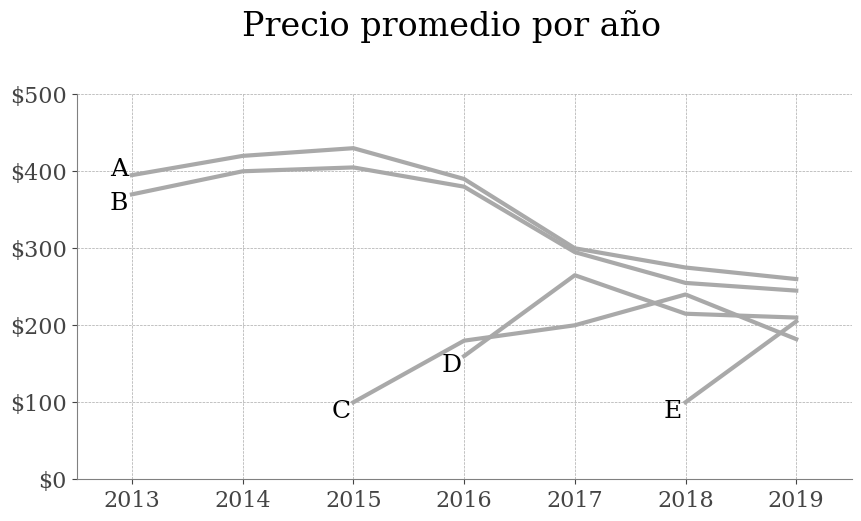
\includegraphics{02_Sol_Sis_Lin_Iter_1_files/figure-pdf/cell-17-output-1.png}

\bookmarksetup{startatroot}

\chapter{\texorpdfstring{Método de Sobrerrelajación sucesiva
(\emph{Successive Overrelaxation},
SOR)}{Método de Sobrerrelajación sucesiva (Successive Overrelaxation, SOR)}}\label{muxe9todo-de-sobrerrelajaciuxf3n-sucesiva-successive-overrelaxation-sor}

\begin{itemize}
\item
  Se obtiene apicando una extrapolación a la iteración de Gauss-Seidel.
\item
  Esta extrapolación es un promedio pesado entre la iteración actual y
  la anterior: \[
  x_i^k = \omega \bar{x}_i^k + (1-\omega)x_i^{k-1}
  \] donde \(\bar{x}\) denota una iteración de Gauss-Seidel y \(\omega\)
  es el factor de extrapolación.
\item
  En términos de matrices tenemos: \$\$ \mathbf{x}\^{}k = (\mathbf{D} -
  \omega \mathbf{L})\^{}\{-1\}(\omega \mathbf{U} + (1 -
  \omega )\mathbf{D})\mathbf{x}\^{}\{k-1\}
\item
  \omega (\mathbf{D} - \omega \mathbf{L})\^{}\{-1\} \mathbf{b} \$\$
\item
  Elegir la \(\omega\) óptima no es simple, aunque se sabe que si
  \(\omega\) está fuera del intervalo \((0,2)\) el método falla.
\end{itemize}

\section{Implementación 3.}\label{implementaciuxf3n-3.}

\begin{Shaded}
\begin{Highlighting}[]
\KeywordTok{def}\NormalTok{ sor(A,b,tol,kmax,w,xi,yi):}
\NormalTok{    N }\OperatorTok{=} \BuiltInTok{len}\NormalTok{(b[}\DecValTok{0}\NormalTok{])}
\NormalTok{    xnew }\OperatorTok{=}\NormalTok{ np.zeros(N)}
\NormalTok{    xold }\OperatorTok{=}\NormalTok{ np.zeros(N)}
\NormalTok{    x }\OperatorTok{=}\NormalTok{ np.array([}\DecValTok{2}\NormalTok{, }\OperatorTok{{-}}\DecValTok{2}\NormalTok{]) }\CommentTok{\# Solución exacta}

    \CommentTok{\# Solución inicial}
\NormalTok{    xold[}\DecValTok{0}\NormalTok{] }\OperatorTok{=}\NormalTok{ xi}
\NormalTok{    xold[}\DecValTok{1}\NormalTok{] }\OperatorTok{=}\NormalTok{ yi}

\NormalTok{    xs }\OperatorTok{=}\NormalTok{ [xi]}
\NormalTok{    ys }\OperatorTok{=}\NormalTok{ [yi]}
    
\NormalTok{    e }\OperatorTok{=} \DecValTok{10}
\NormalTok{    error }\OperatorTok{=}\NormalTok{ [] }
    
\NormalTok{    k }\OperatorTok{=} \DecValTok{0}
    \ControlFlowTok{while}\NormalTok{(e }\OperatorTok{\textgreater{}}\NormalTok{ tol }\KeywordTok{and}\NormalTok{ k }\OperatorTok{\textless{}}\NormalTok{ kmax) :}
        \ControlFlowTok{for}\NormalTok{ i }\KeywordTok{in} \BuiltInTok{range}\NormalTok{(}\DecValTok{0}\NormalTok{,N): }\CommentTok{\# se puede hacer en paralelo}
\NormalTok{            sigma }\OperatorTok{=} \DecValTok{0}
            \ControlFlowTok{for}\NormalTok{ j }\KeywordTok{in} \BuiltInTok{range}\NormalTok{(}\DecValTok{0}\NormalTok{,i):}
\NormalTok{                sigma }\OperatorTok{+=}\NormalTok{ A[i,j] }\OperatorTok{*}\NormalTok{ xnew[j]}
            \ControlFlowTok{for}\NormalTok{ j }\KeywordTok{in} \BuiltInTok{range}\NormalTok{(i}\OperatorTok{+}\DecValTok{1}\NormalTok{,N):}
\NormalTok{                sigma }\OperatorTok{+=}\NormalTok{ A[i,j] }\OperatorTok{*}\NormalTok{ xold[j]                }
\NormalTok{            sigma }\OperatorTok{=}\NormalTok{ (b[}\DecValTok{0}\NormalTok{,i] }\OperatorTok{{-}}\NormalTok{ sigma) }\OperatorTok{/}\NormalTok{ A[i,i]}
\NormalTok{            xnew[i] }\OperatorTok{=}\NormalTok{ xold[i] }\OperatorTok{+}\NormalTok{ w }\OperatorTok{*}\NormalTok{ (sigma }\OperatorTok{{-}}\NormalTok{xold[i])}
            
        \CommentTok{\# Almacenamos la solución actual}
\NormalTok{        xs.append(xnew[}\DecValTok{0}\NormalTok{])}
\NormalTok{        ys.append(xnew[}\DecValTok{1}\NormalTok{])}
        
\NormalTok{        e }\OperatorTok{=}\NormalTok{ np.linalg.norm(xnew}\OperatorTok{{-}}\NormalTok{x, }\DecValTok{2}\NormalTok{) }\CommentTok{\# Cálculo del error}
\NormalTok{        error.append(e)}
\NormalTok{        k }\OperatorTok{+=} \DecValTok{1}
\NormalTok{        xold[:] }\OperatorTok{=}\NormalTok{ xnew[:]}
        \BuiltInTok{print}\NormalTok{(}\StringTok{\textquotesingle{}}\SpecialCharTok{\{:2d\}}\StringTok{ }\SpecialCharTok{\{:10.9f\}}\StringTok{ (}\SpecialCharTok{\{:10.9f\}}\StringTok{, }\SpecialCharTok{\{:10.9f\}}\StringTok{)\textquotesingle{}}\NormalTok{.}\BuiltInTok{format}\NormalTok{(k, e, xnew[}\DecValTok{0}\NormalTok{], xnew[}\DecValTok{1}\NormalTok{]))}
    \ControlFlowTok{return}\NormalTok{ xnew, np.array(xs), np.array(ys), error, k}
\end{Highlighting}
\end{Shaded}

\section{\texorpdfstring{\textbf{Ejercicio
3.}}{Ejercicio 3.}}\label{ejercicio-3.}

Haciendo uso de la función \texttt{sor()} definida en la celda anterior,
aproxima la solución del sistema de ecuaciones del Ejercicio 1. Utiliza
la solución inicial \texttt{(xi,\ yi)\ =} \((-2, 2)\), una tolerancia
\texttt{tol} = \(1 \times 10^{-5}\) y \texttt{kmax} = \(50\)
iteraciones. Elije el valor de \(\omega = 1.09\). Utiliza las variables
\texttt{solSOR}, \texttt{xs}, \texttt{ys}, \texttt{eSOR} e
\texttt{itSOR} para almacenar la salida de la función
\texttt{gauss\_seidel()}. Posteriormente grafica las rectas y cómo se va
calculando la solución con este método (puedes usar el mismo código que
en el caso de Jacobi). Grafica también los errores para los tres métodos
(Jacobi, Gauss-Seidel y SOR).

\textbf{Cálculo de la solución con SOR}

\begin{Shaded}
\begin{Highlighting}[]
\CommentTok{\# Solución inicial}
\CommentTok{\# xi, yi = }
\CommentTok{\# tol = }
\CommentTok{\# kmax = }

\CommentTok{\# Método de SOR, probar con w = 1.09, 1.8, 1.99, 2.0}
\CommentTok{\# w = ...}
\CommentTok{\# ...}

\CommentTok{\#\#\# }\RegionMarkerTok{BEGIN}\CommentTok{ SOLUTION}
\CommentTok{\# Solución inicial}
\NormalTok{xi, yi }\OperatorTok{=} \OperatorTok{{-}}\DecValTok{2}\NormalTok{, }\DecValTok{2}
\NormalTok{tol }\OperatorTok{=} \FloatTok{1e{-}5}
\NormalTok{kmax }\OperatorTok{=} \DecValTok{50}

\CommentTok{\# Método de SOR, probar con w = 1.09, 1.8, 1.99, 2.0}
\NormalTok{w }\OperatorTok{=} \FloatTok{1.09}
\NormalTok{solSOR, xs, ys, eSOR, itSOR }\OperatorTok{=}\NormalTok{ sor(A, b, tol, kmax, w, xi, yi)}

\CommentTok{\#file\_answer.write(\textquotesingle{}7\textquotesingle{}, solSOR, \textquotesingle{}solSOR es incorrecta: revisa la llamada y ejecución de la función sor() así como sus parámetros de entrada.\textquotesingle{})}
\CommentTok{\#file\_answer.write(\textquotesingle{}8\textquotesingle{}, eSOR[{-}1], \textquotesingle{}eSOR[{-}1] es incorrecto: revisa la llamada y ejecución de la función sor() así como sus parámetros de entrada.\textquotesingle{})}
\CommentTok{\#file\_answer.write(\textquotesingle{}9\textquotesingle{}, itSOR, \textquotesingle{}itSOR es incorrector: revisa la llamada y ejecución de la función sor() así como sus parámetros de entrada.\textquotesingle{})}

\CommentTok{\#\#\# }\RegionMarkerTok{END}\CommentTok{ SOLUTION}
\end{Highlighting}
\end{Shaded}

\begin{verbatim}
 1 2.608651498 (-0.546666667, -1.434711111)
 2 0.182203110 (1.818423407, -1.984903171)
 3 0.006309667 (2.005371531, -2.003310371)
 4 0.001963366 (2.001922098, -2.000400429)
 5 0.000118187 (2.000117990, -2.000006831)
 6 0.000006254 (1.999994345, -1.999997330)
\end{verbatim}

\begin{Shaded}
\begin{Highlighting}[]
\CommentTok{\#quizz.eval\_numeric(\textquotesingle{}7\textquotesingle{}, solSOR)}
\CommentTok{\#quizz.eval\_numeric(\textquotesingle{}8\textquotesingle{}, eSOR[{-}1])}
\CommentTok{\#quizz.eval\_numeric(\textquotesingle{}9\textquotesingle{}, itSOR)}
\end{Highlighting}
\end{Shaded}

\textbf{Gráfica de las rectas, la solución y los pasos realizados}

\begin{Shaded}
\begin{Highlighting}[]
\CommentTok{\# Puedes usar el mismo código que en el caso anterior.}

\CommentTok{\#\#\# }\RegionMarkerTok{BEGIN}\CommentTok{ SOLUTION}
\NormalTok{v }\OperatorTok{=}\NormalTok{ mvis.Plotter(}\DecValTok{1}\NormalTok{,}\DecValTok{1}\NormalTok{,[}\BuiltInTok{dict}\NormalTok{(aspect}\OperatorTok{=}\StringTok{\textquotesingle{}equal\textquotesingle{}}\NormalTok{)],title}\OperatorTok{=}\StringTok{\textquotesingle{}Cruce de rectas\textquotesingle{}}\NormalTok{) }
\NormalTok{v.set\_coordsys(}\DecValTok{1}\NormalTok{)}
\NormalTok{v.plot(}\DecValTok{1}\NormalTok{, x, y1, lw }\OperatorTok{=} \DecValTok{3}\NormalTok{, c }\OperatorTok{=} \StringTok{\textquotesingle{}seagreen\textquotesingle{}}\NormalTok{, label }\OperatorTok{=} \StringTok{\textquotesingle{}$3x+2y=2$\textquotesingle{}}\NormalTok{) }\CommentTok{\# Línea recta 1}
\NormalTok{v.plot(}\DecValTok{1}\NormalTok{, x, y2, lw }\OperatorTok{=} \DecValTok{3}\NormalTok{, c }\OperatorTok{=} \StringTok{\textquotesingle{}mediumorchid\textquotesingle{}}\NormalTok{, label }\OperatorTok{=} \StringTok{\textquotesingle{}$2x+6y={-}8$\textquotesingle{}}\NormalTok{) }\CommentTok{\# Línea recta 2}
\NormalTok{v.scatter(}\DecValTok{1}\NormalTok{, sol[}\DecValTok{0}\NormalTok{], sol[}\DecValTok{1}\NormalTok{], fc}\OperatorTok{=}\StringTok{\textquotesingle{}sandybrown\textquotesingle{}}\NormalTok{, ec}\OperatorTok{=}\StringTok{\textquotesingle{}k\textquotesingle{}}\NormalTok{, s }\OperatorTok{=} \DecValTok{75}\NormalTok{, alpha}\OperatorTok{=}\FloatTok{0.75}\NormalTok{, zorder}\OperatorTok{=}\DecValTok{5}\NormalTok{, label}\OperatorTok{=}\StringTok{\textquotesingle{}Sol. final\textquotesingle{}}\NormalTok{) }\CommentTok{\# Solución}

\CommentTok{\# Graficamos los pasos}
\NormalTok{v.scatter(}\DecValTok{1}\NormalTok{, xs[}\DecValTok{0}\NormalTok{], ys[}\DecValTok{0}\NormalTok{], fc}\OperatorTok{=}\StringTok{\textquotesingle{}yellow\textquotesingle{}}\NormalTok{, ec}\OperatorTok{=}\StringTok{\textquotesingle{}k\textquotesingle{}}\NormalTok{, s }\OperatorTok{=} \DecValTok{75}\NormalTok{, alpha}\OperatorTok{=}\FloatTok{0.75}\NormalTok{, zorder}\OperatorTok{=}\DecValTok{8}\NormalTok{, label}\OperatorTok{=}\StringTok{\textquotesingle{}Sol. inicial\textquotesingle{}}\NormalTok{)}
\NormalTok{v.scatter(}\DecValTok{1}\NormalTok{, xs[}\DecValTok{1}\NormalTok{:], ys[}\DecValTok{1}\NormalTok{:], c}\OperatorTok{=}\StringTok{\textquotesingle{}navy\textquotesingle{}}\NormalTok{, s }\OperatorTok{=} \DecValTok{10}\NormalTok{, alpha}\OperatorTok{=}\FloatTok{0.5}\NormalTok{, zorder}\OperatorTok{=}\DecValTok{8}\NormalTok{)}
\NormalTok{v.plot(}\DecValTok{1}\NormalTok{, xs, ys, c}\OperatorTok{=}\StringTok{\textquotesingle{}grey\textquotesingle{}}\NormalTok{, ls }\OperatorTok{=} \StringTok{\textquotesingle{}{-}{-}\textquotesingle{}}\NormalTok{, lw}\OperatorTok{=}\FloatTok{1.0}\NormalTok{, zorder}\OperatorTok{=}\DecValTok{8}\NormalTok{, label}\OperatorTok{=}\StringTok{\textquotesingle{}Pasos del SOR\textquotesingle{}}\NormalTok{)}
        
\NormalTok{v.legend(ncol }\OperatorTok{=} \DecValTok{1}\NormalTok{, frameon}\OperatorTok{=}\VariableTok{True}\NormalTok{, loc}\OperatorTok{=}\StringTok{\textquotesingle{}best\textquotesingle{}}\NormalTok{, bbox\_to\_anchor}\OperatorTok{=}\NormalTok{(}\FloatTok{1.78}\NormalTok{, }\FloatTok{1.01}\NormalTok{))}
\NormalTok{v.grid()}
\NormalTok{v.show()}
\CommentTok{\#\#\# }\RegionMarkerTok{END}\CommentTok{ SOLUTION}
\end{Highlighting}
\end{Shaded}

\includegraphics{02_Sol_Sis_Lin_Iter_1_files/figure-pdf/cell-21-output-1.png}

\begin{Shaded}
\begin{Highlighting}[]
\CommentTok{\# Utiliza el código del caso anterior adaptado para que pueda graficar los tres errores.}

\CommentTok{\#\#\# }\RegionMarkerTok{BEGIN}\CommentTok{ SOLUTION}
\CommentTok{\# Lista con el número de las iteraciones máxima}
\NormalTok{it\_max }\OperatorTok{=} \BuiltInTok{max}\NormalTok{(itJ, itG, itSOR)}\OperatorTok{+}\DecValTok{1}
\NormalTok{l\_it\_max }\OperatorTok{=} \BuiltInTok{list}\NormalTok{(}\BuiltInTok{range}\NormalTok{(}\DecValTok{1}\NormalTok{,it\_max)) }

\CommentTok{\# Listas con el número de las iteraciones para cada algoritmo}
\NormalTok{l\_itJ }\OperatorTok{=} \BuiltInTok{list}\NormalTok{(}\BuiltInTok{range}\NormalTok{(}\DecValTok{1}\NormalTok{,itJ}\OperatorTok{+}\DecValTok{1}\NormalTok{)) }
\NormalTok{l\_itG }\OperatorTok{=} \BuiltInTok{list}\NormalTok{(}\BuiltInTok{range}\NormalTok{(}\DecValTok{1}\NormalTok{,itG}\OperatorTok{+}\DecValTok{1}\NormalTok{)) }
\NormalTok{l\_itSOR }\OperatorTok{=} \BuiltInTok{list}\NormalTok{(}\BuiltInTok{range}\NormalTok{(}\DecValTok{1}\NormalTok{,itSOR}\OperatorTok{+}\DecValTok{1}\NormalTok{)) }

\CommentTok{\# Parámetros para los ejes}
\NormalTok{a\_p }\OperatorTok{=} \BuiltInTok{dict}\NormalTok{(yscale}\OperatorTok{=}\StringTok{\textquotesingle{}log\textquotesingle{}}\NormalTok{, xlabel}\OperatorTok{=}\StringTok{\textquotesingle{}Iteraciones\textquotesingle{}}\NormalTok{, xticks }\OperatorTok{=}\NormalTok{ l\_it\_max)}

\CommentTok{\# Gráficas del error}
\NormalTok{v }\OperatorTok{=}\NormalTok{ mvis.Plotter(}\DecValTok{1}\NormalTok{,}\DecValTok{1}\NormalTok{,[a\_p]) }
\NormalTok{v.axes(}\DecValTok{1}\NormalTok{).set\_title(}\StringTok{\textquotesingle{}Error\textquotesingle{}}\NormalTok{, loc}\OperatorTok{=}\StringTok{\textquotesingle{}left\textquotesingle{}}\NormalTok{)}
\NormalTok{v.plot(}\DecValTok{1}\NormalTok{, l\_itJ, eJ, marker}\OperatorTok{=}\StringTok{\textquotesingle{}.\textquotesingle{}}\NormalTok{, label}\OperatorTok{=}\StringTok{\textquotesingle{}Jacobi\textquotesingle{}}\NormalTok{)}
\NormalTok{v.plot(}\DecValTok{1}\NormalTok{, l\_itG, eG, marker}\OperatorTok{=}\StringTok{\textquotesingle{}.\textquotesingle{}}\NormalTok{, label}\OperatorTok{=}\StringTok{\textquotesingle{}Gauss{-}Seidel\textquotesingle{}}\NormalTok{)}
\NormalTok{v.plot(}\DecValTok{1}\NormalTok{, l\_itSOR, eSOR, marker}\OperatorTok{=}\StringTok{\textquotesingle{}.\textquotesingle{}}\NormalTok{, label}\OperatorTok{=}\StringTok{\textquotesingle{}SOR\textquotesingle{}}\NormalTok{)}
\NormalTok{v.legend()}
\NormalTok{v.grid()}
\CommentTok{\#\#\# }\RegionMarkerTok{END}\CommentTok{ SOLUTION}
\end{Highlighting}
\end{Shaded}

\includegraphics{02_Sol_Sis_Lin_Iter_1_files/figure-pdf/cell-22-output-1.png}

\section{\texorpdfstring{\textbf{Ejercicio
4.}}{Ejercicio 4.}}\label{ejercicio-4.}

Almacena los errores de los tres métodos en los archivos:
\texttt{errorJacobi.npy}, \texttt{errorGaussSeidel.npy} y
\texttt{errorSOR.npy} usando la función \texttt{np.save()}, checa la
documentación
\href{https://numpy.org/doc/stable/reference/generated/numpy.save.html}{aquí}.

Prueba que tu código funciona usando:

\begin{verbatim}
print('Error Jacobi = \n{}\n'.format(np.load('errorJacobi.npy')))
print('Error Gauss-Seidel = \n{}\n'.format(np.load('errorGaussSeidel.npy')))
print('Error SOR = \n{}\n'.format(np.load('errorSOR.npy')))
\end{verbatim}

La salida debería ser:

\begin{verbatim}
Error Jacobi = 
[2.98142397e+00 1.25707872e+00 ...]

Error Gauss-Seidel = 
[2.81091348e+00 6.24647439e-01 ...]

Error SOR = 
[2.60865150e+00 1.82203110e-01 ...]
\end{verbatim}

\begin{Shaded}
\begin{Highlighting}[]
\CommentTok{\# np.save( ... )}
\CommentTok{\#}

\CommentTok{\#\#\# }\RegionMarkerTok{BEGIN}\CommentTok{ SOLUTION}
\NormalTok{np.save(}\StringTok{\textquotesingle{}errorJacobi.npy\textquotesingle{}}\NormalTok{,eJ)}
\NormalTok{np.save(}\StringTok{\textquotesingle{}errorGaussSeidel.npy\textquotesingle{}}\NormalTok{, eG)}
\NormalTok{np.save(}\StringTok{\textquotesingle{}errorSOR.npy\textquotesingle{}}\NormalTok{, eSOR)}
\CommentTok{\#\#\# }\RegionMarkerTok{END}\CommentTok{ SOLUTION}
\end{Highlighting}
\end{Shaded}

\begin{Shaded}
\begin{Highlighting}[]
\BuiltInTok{print}\NormalTok{(}\StringTok{\textquotesingle{}Error Jacobi = }\CharTok{\textbackslash{}n}\SpecialCharTok{\{\}}\CharTok{\textbackslash{}n}\StringTok{\textquotesingle{}}\NormalTok{.}\BuiltInTok{format}\NormalTok{(np.load(}\StringTok{\textquotesingle{}errorJacobi.npy\textquotesingle{}}\NormalTok{)))}
\BuiltInTok{print}\NormalTok{(}\StringTok{\textquotesingle{}Error Gauss{-}Seidel = }\CharTok{\textbackslash{}n}\SpecialCharTok{\{\}}\CharTok{\textbackslash{}n}\StringTok{\textquotesingle{}}\NormalTok{.}\BuiltInTok{format}\NormalTok{(np.load(}\StringTok{\textquotesingle{}errorGaussSeidel.npy\textquotesingle{}}\NormalTok{)))}
\BuiltInTok{print}\NormalTok{(}\StringTok{\textquotesingle{}Error SOR = }\CharTok{\textbackslash{}n}\SpecialCharTok{\{\}}\CharTok{\textbackslash{}n}\StringTok{\textquotesingle{}}\NormalTok{.}\BuiltInTok{format}\NormalTok{(np.load(}\StringTok{\textquotesingle{}errorSOR.npy\textquotesingle{}}\NormalTok{)))}
\end{Highlighting}
\end{Shaded}

\begin{verbatim}
Error Jacobi = 
[2.98142397e+00 1.25707872e+00 6.62538660e-01 2.79350827e-01
 1.47230813e-01 6.20779616e-02 3.27179585e-02 1.37951026e-02
 7.27065745e-03 3.06557835e-03 1.61570166e-03 6.81239633e-04
 3.59044812e-04 1.51386585e-04 7.97877361e-05 3.36414634e-05
 1.77306080e-05 7.47588075e-06]

Error Gauss-Seidel = 
[2.81091348e+00 6.24647439e-01 1.38810542e-01 3.08467871e-02
 6.85484158e-03 1.52329813e-03 3.38510695e-04 7.52245990e-05
 1.67165775e-05 3.71479501e-06]

Error SOR = 
[2.60865150e+00 1.82203110e-01 6.30966741e-03 1.96336589e-03
 1.18187146e-04 6.25365681e-06]
\end{verbatim}

\bookmarksetup{startatroot}

\chapter{Descenso del gradiente y Gradiente
Conjugado.}\label{descenso-del-gradiente-y-gradiente-conjugado.}

\textbf{Objetivo.}

Describir e implementar los métodos de descenso del gradiente y de
gradiente conjugado para la solución de sistemas de ecuaciones lineales.

MACTI-Algebra\_Lineal\_01 by Luis M. de la Cruz is licensed under
Attribution-ShareAlike 4.0 International

Trabajo realizado con el apoyo del Programa UNAM-DGAPA-PAPIME PE101922

\begin{Shaded}
\begin{Highlighting}[]
\ImportTok{import}\NormalTok{ numpy }\ImportTok{as}\NormalTok{ np}
\ImportTok{import}\NormalTok{ ipywidgets }\ImportTok{as}\NormalTok{ widgets}
\ImportTok{import}\NormalTok{ macti.visual }\ImportTok{as}\NormalTok{ mvis}
\ImportTok{import}\NormalTok{ macti.matem }\ImportTok{as}\NormalTok{ mmat}
\end{Highlighting}
\end{Shaded}

La siguiente función será usada para graficar algunos resultados.

\begin{Shaded}
\begin{Highlighting}[]
\KeywordTok{def}\NormalTok{ grafica(x, y1, y2, sol }\OperatorTok{=}\NormalTok{ [], xs }\OperatorTok{=}\NormalTok{ [], ys }\OperatorTok{=}\NormalTok{ [], vA }\OperatorTok{=}\NormalTok{ [], xg }\OperatorTok{=}\NormalTok{ [], yg }\OperatorTok{=}\NormalTok{ [], z }\OperatorTok{=}\NormalTok{ []):}
    \CommentTok{"""}
\CommentTok{    Esta función grafica las líneas rectas, la solución, los pasos y los eigenvectores.}
\CommentTok{    """}
\NormalTok{    v }\OperatorTok{=}\NormalTok{ mvis.Plotter(}\DecValTok{1}\NormalTok{,}\DecValTok{1}\NormalTok{,[}\BuiltInTok{dict}\NormalTok{(aspect}\OperatorTok{=}\StringTok{\textquotesingle{}equal\textquotesingle{}}\NormalTok{)],title}\OperatorTok{=}\StringTok{\textquotesingle{}Cruce de rectas\textquotesingle{}}\NormalTok{) }
\NormalTok{    v.set\_coordsys(}\DecValTok{1}\NormalTok{)}
    
    \CommentTok{\# Graficamos las líneas rectas}
\NormalTok{    v.plot(}\DecValTok{1}\NormalTok{, x, y1, lw }\OperatorTok{=} \DecValTok{3}\NormalTok{, c }\OperatorTok{=} \StringTok{\textquotesingle{}seagreen\textquotesingle{}}\NormalTok{, label }\OperatorTok{=} \StringTok{\textquotesingle{}$3x+2y=2$\textquotesingle{}}\NormalTok{) }\CommentTok{\# Línea recta 1}
\NormalTok{    v.plot(}\DecValTok{1}\NormalTok{, x, y2, lw }\OperatorTok{=} \DecValTok{3}\NormalTok{, c }\OperatorTok{=} \StringTok{\textquotesingle{}mediumorchid\textquotesingle{}}\NormalTok{, label }\OperatorTok{=} \StringTok{\textquotesingle{}$2x+6y={-}8$\textquotesingle{}}\NormalTok{) }\CommentTok{\# Línea recta 2}

    \ControlFlowTok{if} \BuiltInTok{len}\NormalTok{(sol):}
        \CommentTok{\# Graficamos la solución}
\NormalTok{        v.scatter(}\DecValTok{1}\NormalTok{, sol[}\DecValTok{0}\NormalTok{], sol[}\DecValTok{1}\NormalTok{], fc}\OperatorTok{=}\StringTok{\textquotesingle{}sandybrown\textquotesingle{}}\NormalTok{, ec}\OperatorTok{=}\StringTok{\textquotesingle{}k\textquotesingle{}}\NormalTok{, s }\OperatorTok{=} \DecValTok{75}\NormalTok{, alpha}\OperatorTok{=}\FloatTok{0.75}\NormalTok{, zorder}\OperatorTok{=}\DecValTok{5}\NormalTok{, label}\OperatorTok{=}\StringTok{\textquotesingle{}Solución final         .\textquotesingle{}}\NormalTok{) }\CommentTok{\# Solución}

    \ControlFlowTok{if} \BuiltInTok{len}\NormalTok{(xs) }\KeywordTok{and} \BuiltInTok{len}\NormalTok{(ys):}
        \CommentTok{\# Graficamos los pasos}
\NormalTok{        v.scatter(}\DecValTok{1}\NormalTok{, xs[}\DecValTok{0}\NormalTok{], ys[}\DecValTok{0}\NormalTok{], fc}\OperatorTok{=}\StringTok{\textquotesingle{}yellow\textquotesingle{}}\NormalTok{, ec}\OperatorTok{=}\StringTok{\textquotesingle{}k\textquotesingle{}}\NormalTok{, s }\OperatorTok{=} \DecValTok{75}\NormalTok{, alpha}\OperatorTok{=}\FloatTok{0.75}\NormalTok{, zorder}\OperatorTok{=}\DecValTok{8}\NormalTok{, label}\OperatorTok{=}\StringTok{\textquotesingle{}Solución inicial\textquotesingle{}}\NormalTok{)}
\NormalTok{        v.scatter(}\DecValTok{1}\NormalTok{, xs[}\DecValTok{1}\NormalTok{:], ys[}\DecValTok{1}\NormalTok{:], c}\OperatorTok{=}\StringTok{\textquotesingle{}navy\textquotesingle{}}\NormalTok{, s }\OperatorTok{=} \DecValTok{10}\NormalTok{, alpha}\OperatorTok{=}\FloatTok{0.5}\NormalTok{, zorder}\OperatorTok{=}\DecValTok{8}\NormalTok{)}
\NormalTok{        v.plot(}\DecValTok{1}\NormalTok{, xs, ys, c}\OperatorTok{=}\StringTok{\textquotesingle{}grey\textquotesingle{}}\NormalTok{, ls }\OperatorTok{=} \StringTok{\textquotesingle{}{-}{-}\textquotesingle{}}\NormalTok{, lw}\OperatorTok{=}\FloatTok{1.0}\NormalTok{, zorder}\OperatorTok{=}\DecValTok{8}\NormalTok{, label}\OperatorTok{=}\StringTok{\textquotesingle{}Pasos del método\textquotesingle{}}\NormalTok{)}

    \ControlFlowTok{if} \BuiltInTok{len}\NormalTok{(vA):}
        \CommentTok{\# Graficamos los eigenvectores}
\NormalTok{        v.quiver(}\DecValTok{1}\NormalTok{, [sol[}\DecValTok{0}\NormalTok{], sol[}\DecValTok{0}\NormalTok{]], [sol[}\DecValTok{1}\NormalTok{], sol[}\DecValTok{1}\NormalTok{]], vA[}\DecValTok{0}\NormalTok{], vA[}\DecValTok{1}\NormalTok{], scale}\OperatorTok{=}\DecValTok{10}\NormalTok{, zorder}\OperatorTok{=}\DecValTok{9}\NormalTok{)}

    \ControlFlowTok{if} \BuiltInTok{len}\NormalTok{(xg) }\KeywordTok{and} \BuiltInTok{len}\NormalTok{(yg) }\KeywordTok{and} \BuiltInTok{len}\NormalTok{(z):}
\NormalTok{        v.contour(}\DecValTok{1}\NormalTok{, xg, yg, z, levels }\OperatorTok{=} \DecValTok{25}\NormalTok{, cmap}\OperatorTok{=}\StringTok{\textquotesingle{}twilight\textquotesingle{}}\NormalTok{, linewidths}\OperatorTok{=}\FloatTok{1.0}\NormalTok{, zorder}\OperatorTok{=}\DecValTok{1}\NormalTok{)        }
        
\NormalTok{    v.legend(ncol }\OperatorTok{=} \DecValTok{1}\NormalTok{, frameon}\OperatorTok{=}\VariableTok{True}\NormalTok{, loc}\OperatorTok{=}\StringTok{\textquotesingle{}best\textquotesingle{}}\NormalTok{, bbox\_to\_anchor}\OperatorTok{=}\NormalTok{(}\FloatTok{1.90}\NormalTok{, }\FloatTok{1.02}\NormalTok{))}
\NormalTok{    v.grid()}
\NormalTok{    v.show()}
\end{Highlighting}
\end{Shaded}

\section{\texorpdfstring{\textbf{Ejemplo 1. Cruce de líneas
rectas.}}{Ejemplo 1. Cruce de líneas rectas.}}\label{ejemplo-1.-cruce-de-luxedneas-rectas.}

Las siguientes dos rectas se cruzan en algún punto.

\[
\begin{array}{ccc}
3x + 2y & = &2 \\
2x + 6y & = &-8
\end{array}
\]

Las ecuaciones de las rectas se pueden escribir como:

\[
\begin{array}{ccc}
\dfrac{3}{2}x + y & = & 1 \\
\dfrac{2}{6}x + y & = & -\dfrac{8}{6}
\end{array} \Longrightarrow
\begin{array}{ccc}
y = m_1 x + b_1 \\
y = m_2 x + b_2
\end{array} \text{ donde }
\begin{array}{ccc}
m_1 = -\dfrac{3}{2} & b_1 = 1 \\
m_2 = -\dfrac{2}{6} & b_2 = -\dfrac{8}{6}
\end{array}
\]

Las ecuaciones de las rectas se pueden escribir en forma de un sistema
lineal:

\[
\left[
\begin{array}{cc}
3 & 2 \\
2 & 6
\end{array} \right]
\left[
\begin{array}{c}
x_{0} \\
x_{1}
\end{array} \right] =
\left[
\begin{array}{c}
2 \\ 
-8
\end{array} \right]
\tag{1}
\]

Podemos calcular el cruce de las rectas resolviendo el sistema lineal:

\begin{Shaded}
\begin{Highlighting}[]
\CommentTok{\# Dominio}
\NormalTok{x }\OperatorTok{=}\NormalTok{ np.linspace(}\OperatorTok{{-}}\DecValTok{3}\NormalTok{,}\DecValTok{6}\NormalTok{,}\DecValTok{10}\NormalTok{)}

\CommentTok{\# Línea recta 1}
\NormalTok{m1 }\OperatorTok{=} \OperatorTok{{-}}\DecValTok{3}\OperatorTok{/}\DecValTok{2}
\NormalTok{b1 }\OperatorTok{=} \DecValTok{1}
\NormalTok{y1 }\OperatorTok{=}\NormalTok{ m1 }\OperatorTok{*}\NormalTok{ x }\OperatorTok{+}\NormalTok{ b1}

\CommentTok{\# Línea recta 2}
\NormalTok{m2 }\OperatorTok{=} \OperatorTok{{-}}\DecValTok{2}\OperatorTok{/}\DecValTok{6}
\NormalTok{b2 }\OperatorTok{=} \OperatorTok{{-}}\DecValTok{8}\OperatorTok{/}\DecValTok{6}
\NormalTok{y2 }\OperatorTok{=}\NormalTok{ m2 }\OperatorTok{*}\NormalTok{ x }\OperatorTok{+}\NormalTok{ b2 }

\CommentTok{\# Definimos el sistema de ecuaciones lineales}
\NormalTok{A }\OperatorTok{=}\NormalTok{ np.array([[}\DecValTok{3}\NormalTok{, }\DecValTok{2}\NormalTok{],[}\DecValTok{2}\NormalTok{,}\DecValTok{6}\NormalTok{]] )}
\NormalTok{b }\OperatorTok{=}\NormalTok{ np.array([}\DecValTok{2}\NormalTok{,}\OperatorTok{{-}}\DecValTok{8}\NormalTok{])}
\BuiltInTok{print}\NormalTok{(}\StringTok{"Matriz A : }\CharTok{\textbackslash{}n}\StringTok{"}\NormalTok{,A)}
\BuiltInTok{print}\NormalTok{(}\StringTok{"Vector b : }\CharTok{\textbackslash{}n}\StringTok{"}\NormalTok{, b)}

\CommentTok{\# Resolvemos el sistema}
\NormalTok{sol }\OperatorTok{=}\NormalTok{ np.linalg.solve(A,b)}
\BuiltInTok{print}\NormalTok{(}\StringTok{"Solución del sistema: "}\NormalTok{, sol)}

\CommentTok{\# Usamos la función grafica() para mostrar las rectas y la solución}
\NormalTok{grafica(x, y1, y2, sol)}
\end{Highlighting}
\end{Shaded}

\begin{verbatim}
Matriz A : 
 [[3 2]
 [2 6]]
Vector b : 
 [ 2 -8]
Solución del sistema:  [ 2. -2.]
\end{verbatim}

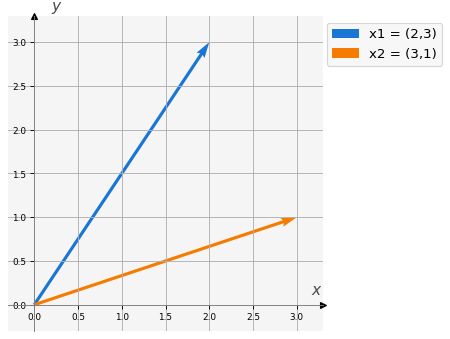
\includegraphics{03_Sol_Sis_Lin_Krylov_files/figure-pdf/cell-4-output-2.png}

En general, un sistema de ecuaciones de \(n \times n\) se escribe como
sigue:

\[
\begin{array}{ccccccc}
a_{11}x_1 & + & a_{12}x_2 & +  \dots  + & a_{1n}x_n & = & b_1 \\
a_{21}x_1 & + & a_{22}x_2 & +  \dots + & a_{2n}x_n & = & b_2 \\
\vdots & & \vdots &  & \vdots & & \vdots \\
a_{i1}x_1 & + & a_{i2}x_2 & +  \dots + & a_{in}x_n & = & b_i \\
\vdots & & \vdots &  & \vdots & & \vdots \\
a_{n1}x_1 & + & a_{n2}x_2 & + \dots + & a_{nn}x_n & = & b_n
\end{array}
\]

Es posible usar métodos más eficientes que el de Jacobi, Gauss-Seidel y
SOR para resolver este tipo de sistemas. A continuación veremos los
métodos del descenso del gradiente y método de gradiente conjugado.

\bookmarksetup{startatroot}

\chapter{Métodos del subespacio de
Krylov}\label{muxe9todos-del-subespacio-de-krylov}

Una excelente referencia para comenzar con estos métodos es la
siguiente:

Shewchuk, J. R. (1994).
\href{https://www.cs.cmu.edu/~quake-papers/painless-conjugate-gradient.pdf}{An
Introduction to the Conjugate Gradient Method Without the Agonizing
Pain}. Carnegie-Mellon University. Department of Computer Science.

\section{Cálculo de eigenvectores}\label{cuxe1lculo-de-eigenvectores}

Los eigenvalores y eigenvectores de una matriz son herramientas muy
útiles para entender ciertos comportamientos. Una descripción la puedes
ver en la notebook \url{05_Matrices_Normas_Eigen.ipynb}. Los
eigenvalores y eigenvectores se pueden calcular como sigue:

\begin{Shaded}
\begin{Highlighting}[]
\CommentTok{\# Usando la función np.linalg.eig()}
\NormalTok{np.linalg.eig(A)  }\CommentTok{\# w: eigenvalues, v: eigenvectors}
\end{Highlighting}
\end{Shaded}

\begin{verbatim}
EigResult(eigenvalues=array([2., 7.]), eigenvectors=array([[-0.89442719, -0.4472136 ],
       [ 0.4472136 , -0.89442719]]))
\end{verbatim}

La función \texttt{eigen\_land()} de la biblioteca \texttt{macti}
utiliza la función \texttt{np.linalg.eig()} para ofrecer una salida más
entendible:

\begin{Shaded}
\begin{Highlighting}[]
\CommentTok{\# Usando la función eigen\_land() de macti}
\NormalTok{wA, vA }\OperatorTok{=}\NormalTok{ mmat.eigen\_land(A)}
\end{Highlighting}
\end{Shaded}

\begin{verbatim}
eigenvalores = [2. 7.]
eigenvectores:
 [-0.89442719  0.4472136 ] 
 [-0.4472136  -0.89442719]
ángulo entre eigenvectores = 90.0
\end{verbatim}

Los eigenvectores se pueden visualizar, cuando la matriz es de
\(2\times2\):

\begin{Shaded}
\begin{Highlighting}[]
\CommentTok{\# Graficamos los eigenvectores}
\NormalTok{xv }\OperatorTok{=}\NormalTok{ np.array([[sol[}\DecValTok{0}\NormalTok{], sol[}\DecValTok{0}\NormalTok{]],}
\NormalTok{               [sol[}\DecValTok{1}\NormalTok{], sol[}\DecValTok{1}\NormalTok{]]])}

\NormalTok{v }\OperatorTok{=}\NormalTok{ mvis.Plotter() }
\NormalTok{v.quiver(}\DecValTok{1}\NormalTok{, xv[}\DecValTok{0}\NormalTok{], xv[}\DecValTok{1}\NormalTok{], vA[}\DecValTok{0}\NormalTok{], vA[}\DecValTok{1}\NormalTok{], scale}\OperatorTok{=}\DecValTok{10}\NormalTok{, zorder}\OperatorTok{=}\DecValTok{6}\NormalTok{)}
\NormalTok{v.grid()}
\NormalTok{v.show()}
\end{Highlighting}
\end{Shaded}

\includegraphics{03_Sol_Sis_Lin_Krylov_files/figure-pdf/cell-7-output-1.png}

Ahora usamos la función \texttt{grafica()} definida al principio de esta
notebook para ver los eigenvectores y las líneas rectas:

\begin{Shaded}
\begin{Highlighting}[]
\CommentTok{\# Usamos la función grafica() para ver los eigenvectores}
\NormalTok{grafica(x,y1,y2,sol,vA}\OperatorTok{=}\NormalTok{vA)}
\end{Highlighting}
\end{Shaded}

\includegraphics{03_Sol_Sis_Lin_Krylov_files/figure-pdf/cell-8-output-1.png}

\section{Forma cuadrática}\label{forma-cuadruxe1tica}

La forma cuadrática de un sistema de ecuaciones lineales, permite
transformar el problema \(A \mathbf{x} = \mathbf{b}\) en un probema de
minimización.

\[ f(\mathbf{x}) = \dfrac{1}{2} \mathbf{x}^T A \mathbf{x} - \mathbf{x}^T \mathbf{b} + \mathbf{c} \]

\[
A =
\left[
\begin{array}{cc}
3 & 2 \\
2 & 6
\end{array} \right],
\mathbf{x} =
\left[
\begin{array}{c}
x_{0} \\
x_{1}
\end{array} \right],
\mathbf{b} =
\left[
\begin{array}{c}
2\\ -8
\end{array}
\right], 
\mathbf{c} =
\left[
\begin{array}{c}
0\\ 0
\end{array}
\right], 
\]

\[ f^\prime(\mathbf{x}) = \dfrac{1}{2} A^T \mathbf{x} + \dfrac{1}{2} A \mathbf{x} - \mathbf{b} \]

\begin{itemize}
\tightlist
\item
  Cuando \(A\) es simétrica: \$ f\^{}\prime(\mathbf{x}) = A \mathbf{x} -
  \mathbf{b} \$
\item
  Entonces un punto crítico de \(f(\mathbf{x})\) se obtiene cuando \$
  f\^{}\prime(\mathbf{x}) = A \mathbf{x} - \mathbf{b} = 0\$, es decir
  cuando \(A \mathbf{x} = \mathbf{b}\)
\end{itemize}

Calculemos la forma cuadrática para nuestro ejemplo:

\begin{Shaded}
\begin{Highlighting}[]
\CommentTok{\# Función cuadrática}
\NormalTok{f }\OperatorTok{=} \KeywordTok{lambda}\NormalTok{ A,b,c,x: }\FloatTok{0.5} \OperatorTok{*}\NormalTok{ x }\OperatorTok{@}\NormalTok{ A }\OperatorTok{@}\NormalTok{ x.T }\OperatorTok{{-}}\NormalTok{ x }\OperatorTok{@}\NormalTok{ b.T }\OperatorTok{+}\NormalTok{ c}

\CommentTok{\# Tamaño de la malla para graficar}
\NormalTok{size\_grid }\OperatorTok{=} \DecValTok{30}
\NormalTok{xg, yg }\OperatorTok{=}\NormalTok{ np.meshgrid(np.linspace(}\OperatorTok{{-}}\DecValTok{3}\NormalTok{,}\DecValTok{6}\NormalTok{,size\_grid),}
\NormalTok{                     np.linspace(}\OperatorTok{{-}}\DecValTok{8}\NormalTok{,}\DecValTok{6}\NormalTok{,size\_grid))}

\CommentTok{\# Arreglo para almacenar los valores de la función cuadrática}
\NormalTok{z }\OperatorTok{=}\NormalTok{ np.zeros((size\_grid, size\_grid))}

\CommentTok{\# Cálculo}
\ControlFlowTok{for}\NormalTok{ i }\KeywordTok{in} \BuiltInTok{range}\NormalTok{(size\_grid):}
    \ControlFlowTok{for}\NormalTok{ j }\KeywordTok{in} \BuiltInTok{range}\NormalTok{(size\_grid):}
\NormalTok{        xc }\OperatorTok{=}\NormalTok{ np.array([[xg[i,j], yg[i,j]]])}
\NormalTok{        z[i,j] }\OperatorTok{=}\NormalTok{ f(A,b,}\DecValTok{0}\NormalTok{,xc)}
\end{Highlighting}
\end{Shaded}

\begin{verbatim}
/tmp/ipykernel_217/3515168418.py:16: DeprecationWarning: Conversion of an array with ndim > 0 to a scalar is deprecated, and will error in future. Ensure you extract a single element from your array before performing this operation. (Deprecated NumPy 1.25.)
  z[i,j] = f(A,b,0,xc)
\end{verbatim}

Graficamos la forma cuadrática, almacenada en \texttt{z}, y la solución.
Esta última debe estar en el mínimo de \(f(\mathbf{x})\).

\begin{Shaded}
\begin{Highlighting}[]
\NormalTok{axis\_par }\OperatorTok{=}\NormalTok{ [}\BuiltInTok{dict}\NormalTok{(projection}\OperatorTok{=}\StringTok{\textquotesingle{}3d\textquotesingle{}}\NormalTok{, aspect}\OperatorTok{=}\StringTok{\textquotesingle{}auto\textquotesingle{}}\NormalTok{, xlabel }\OperatorTok{=} \StringTok{\textquotesingle{}$x$\textquotesingle{}}\NormalTok{, ylabel }\OperatorTok{=} \StringTok{\textquotesingle{}$y$\textquotesingle{}}\NormalTok{, zlabel }\OperatorTok{=} \StringTok{\textquotesingle{}$f$\textquotesingle{}}\NormalTok{)]}
\NormalTok{v }\OperatorTok{=}\NormalTok{ mvis.Plotter(}\DecValTok{1}\NormalTok{,}\DecValTok{1}\NormalTok{, axis\_par, }\BuiltInTok{dict}\NormalTok{(figsize}\OperatorTok{=}\NormalTok{(}\DecValTok{8}\NormalTok{,}\DecValTok{6}\NormalTok{)))}
\NormalTok{v.plot\_surface(}\DecValTok{1}\NormalTok{, xg, yg, z, cmap}\OperatorTok{=}\StringTok{\textquotesingle{}twilight\textquotesingle{}}\NormalTok{, alpha}\OperatorTok{=}\FloatTok{0.90}\NormalTok{) }\CommentTok{\# f(x)}
\NormalTok{v.scatter(}\DecValTok{1}\NormalTok{, sol[}\DecValTok{0}\NormalTok{], sol[}\DecValTok{1}\NormalTok{], fc}\OperatorTok{=}\StringTok{\textquotesingle{}sandybrown\textquotesingle{}}\NormalTok{, ec}\OperatorTok{=}\StringTok{\textquotesingle{}k\textquotesingle{}}\NormalTok{, s }\OperatorTok{=} \DecValTok{75}\NormalTok{, zorder}\OperatorTok{=}\DecValTok{5}\NormalTok{, label}\OperatorTok{=}\StringTok{\textquotesingle{}Solución\textquotesingle{}}\NormalTok{)}
\NormalTok{v.axes(}\DecValTok{1}\NormalTok{).view\_init(elev }\OperatorTok{=} \DecValTok{15}\NormalTok{, azim }\OperatorTok{=} \OperatorTok{{-}}\DecValTok{15}\NormalTok{)}
\end{Highlighting}
\end{Shaded}

\includegraphics{03_Sol_Sis_Lin_Krylov_files/figure-pdf/cell-10-output-1.png}

Observamos un paraboloide cuyo mínimo es la solución del sistema. Esto
es más claro si graficamos los contornos de \(f(\mathbf{x})\):

\begin{Shaded}
\begin{Highlighting}[]
\NormalTok{grafica(x, y1, y2, sol, vA }\OperatorTok{=}\NormalTok{ vA, xg }\OperatorTok{=}\NormalTok{ xg, yg }\OperatorTok{=}\NormalTok{ yg, z }\OperatorTok{=}\NormalTok{ z)}
\end{Highlighting}
\end{Shaded}

\includegraphics{03_Sol_Sis_Lin_Krylov_files/figure-pdf/cell-11-output-1.png}

\section{Algoritmo de descenso por el
gradiente.}\label{algoritmo-de-descenso-por-el-gradiente.}

Este algoritmo utiliza la dirección del gradiente, en sentido negativo,
para encontrar el mínimo y la solución del sistema:

\$

\begin{array}{l}
\text{Input} : \mathbf{x}_0, tol \\
\mathbf{r}_0 = \mathbf{b}-A\mathbf{x}_0 \\
k = 0 \\
\text{WHILE}(\mathbf{r}_k > tol) \\
\qquad \mathbf{r}_k \leftarrow \mathbf{b}-A\mathbf{x}_k \\
\qquad \alpha_k \leftarrow \dfrac{\mathbf{r}_k^T\mathbf{r}_k}{\mathbf{r}_k^T A \mathbf{r}_k} \\
\qquad \mathbf{x}_{k+1} \leftarrow \mathbf{x}_k + \alpha_k \mathbf{r}_k \\
\qquad k \leftarrow k + 1 \\
\text{ENDWHILE}
\end{array}

\$

\section{Implementación.}\label{implementaciuxf3n.-2}

\begin{Shaded}
\begin{Highlighting}[]
\KeywordTok{def}\NormalTok{ steepest(A,b,xi, yi,tol,kmax):}
    \CommentTok{\# Solución inicial en forma de vector}
\NormalTok{    x }\OperatorTok{=}\NormalTok{ np.array([xi, yi]) }
    
    \CommentTok{\# Arreglos para almacenar los pasos.}
\NormalTok{    xs, ys }\OperatorTok{=}\NormalTok{ [xi], [yi]}
    
    \CommentTok{\# Solución exacta}
\NormalTok{    xe }\OperatorTok{=}\NormalTok{ np.array([}\DecValTok{2}\NormalTok{, }\OperatorTok{{-}}\DecValTok{2}\NormalTok{]) }
                  
\NormalTok{    r }\OperatorTok{=}\NormalTok{ b.T }\OperatorTok{{-}}\NormalTok{ A }\OperatorTok{@}\NormalTok{ x}
\NormalTok{    res }\OperatorTok{=}\NormalTok{ np.linalg.norm(r, }\DecValTok{2}\NormalTok{)}
\NormalTok{    res\_list }\OperatorTok{=}\NormalTok{ []}
\NormalTok{    error }\OperatorTok{=}\NormalTok{ []}
\NormalTok{    k }\OperatorTok{=} \DecValTok{0}
    \ControlFlowTok{while}\NormalTok{(res }\OperatorTok{\textgreater{}}\NormalTok{ tol }\KeywordTok{and}\NormalTok{ k }\OperatorTok{\textless{}}\NormalTok{ kmax):}
\NormalTok{        alpha }\OperatorTok{=}\NormalTok{ r.T }\OperatorTok{@}\NormalTok{ r }\OperatorTok{/}\NormalTok{ (r.T }\OperatorTok{@}\NormalTok{ A }\OperatorTok{@}\NormalTok{ r)}
\NormalTok{        x }\OperatorTok{=}\NormalTok{ x }\OperatorTok{+}\NormalTok{ r }\OperatorTok{*}\NormalTok{ alpha}
\NormalTok{        xs.append(x[}\DecValTok{0}\NormalTok{])}
\NormalTok{        ys.append(x[}\DecValTok{1}\NormalTok{])}
\NormalTok{        r }\OperatorTok{=}\NormalTok{ b.T }\OperatorTok{{-}}\NormalTok{ A }\OperatorTok{@}\NormalTok{ x}
        
        \CommentTok{\# Resido}
\NormalTok{        res }\OperatorTok{=}\NormalTok{ np.linalg.norm(r, }\DecValTok{2}\NormalTok{)}
\NormalTok{        res\_list.append(res)}
        
        \CommentTok{\# Error}
\NormalTok{        e }\OperatorTok{=}\NormalTok{ np.linalg.norm(np.array([x[}\DecValTok{0}\NormalTok{], x[}\DecValTok{1}\NormalTok{]]) }\OperatorTok{{-}}\NormalTok{ xe, }\DecValTok{2}\NormalTok{)}
\NormalTok{        error.append(e)}
        
\NormalTok{        k }\OperatorTok{+=} \DecValTok{1}
        \BuiltInTok{print}\NormalTok{(}\StringTok{\textquotesingle{}}\SpecialCharTok{\{:2d\}}\StringTok{ }\SpecialCharTok{\{:10.9f\}}\StringTok{ (}\SpecialCharTok{\{:10.9f\}}\StringTok{, }\SpecialCharTok{\{:10.9f\}}\StringTok{)\textquotesingle{}}\NormalTok{.}\BuiltInTok{format}\NormalTok{(k, e, x[}\DecValTok{0}\NormalTok{], x[}\DecValTok{1}\NormalTok{]))}
    \ControlFlowTok{return}\NormalTok{ x, np.array(xs), np.array(ys), error, res\_list, k }
\end{Highlighting}
\end{Shaded}

\section{\texorpdfstring{\textbf{Ejercicio
1.}}{Ejercicio 1.}}\label{ejercicio-1.-1}

Haciendo uso de la función \texttt{steepest()} definida en la celda
anterior, aproxima la solución del sistema de ecuaciones del Ejemplo 1.
Utiliza la solución inicial \texttt{(xi,\ yi)\ =} \((-2, 2)\), una
tolerancia \texttt{tol} = \(1 \times 10^{-5}\) y \texttt{kmax} = \(50\)
iteraciones. Utiliza las variables \texttt{solGrad}, \texttt{xs},
\texttt{ys}, \texttt{eGrad}, \texttt{rGrad} e \texttt{itGrad} para
almacenar la salida de la función \texttt{steepest()}. Posteriormente
grafica las rectas y cómo se va calculando la solución con este método.
Utiliza la función \texttt{grafica()}. Grafica también el error y el
residuo.

\begin{Shaded}
\begin{Highlighting}[]
\CommentTok{\# Solución inicial (debe darse como un arreglo tipo columna)}
\CommentTok{\# (xi, yi) = ...}

\CommentTok{\# Método Steepest descend}
\CommentTok{\# ...}

\CommentTok{\#\#\# }\RegionMarkerTok{BEGIN}\CommentTok{ SOLUTION}
\CommentTok{\# Solución inicial}
\NormalTok{(xi, yi) }\OperatorTok{=}\NormalTok{ (}\OperatorTok{{-}}\FloatTok{2.}\NormalTok{, }\FloatTok{2.}\NormalTok{)}
\NormalTok{tol }\OperatorTok{=} \FloatTok{1e{-}5}
\NormalTok{kmax }\OperatorTok{=} \DecValTok{50}

\CommentTok{\# Método Steepest descend}
\NormalTok{solGrad, xs, ys, eGrad, rGrad, itGrad  }\OperatorTok{=}\NormalTok{ steepest(A, b, xi, yi, tol, kmax)}

\CommentTok{\#file\_answer.write(\textquotesingle{}1\textquotesingle{}, solGrad, \textquotesingle{}solGrad es incorrecta: revisa la llamada y ejecución de la función steepest() así como sus parámetros de entrada.\textquotesingle{})}
\CommentTok{\#file\_answer.write(\textquotesingle{}2\textquotesingle{}, eGrad[{-}1], \textquotesingle{}eGrad[{-}1] es incorrecto: revisa la llamada y ejecución de la función steepest() así como sus parámetros de entrada.\textquotesingle{})}
\CommentTok{\#file\_answer.write(\textquotesingle{}3\textquotesingle{}, rGrad[{-}1], \textquotesingle{}rGrad[{-}1] es incorrecto: revisa la llamada y ejecución de la función steepest() así como sus parámetros de entrada.\textquotesingle{})}
\CommentTok{\#file\_answer.write(\textquotesingle{}4\textquotesingle{}, itGrad, \textquotesingle{}itGrad es incorrecto: revisa la llamada y ejecución de la función steepest() así como sus parámetros de entrada.\textquotesingle{})}

\CommentTok{\#\#\# }\RegionMarkerTok{END}\CommentTok{ SOLUTION}
\end{Highlighting}
\end{Shaded}

\begin{verbatim}
 1 3.261835423 (-1.180722892, -1.277108434)
 2 1.717502736 (0.785542169, -0.785542169)
 3 0.990340394 (1.034286544, -1.780519669)
 4 0.521458662 (1.631273044, -1.631273044)
 5 0.300681662 (1.706795433, -1.933362598)
 6 0.158322389 (1.888049165, -1.888049165)
 7 0.091291300 (1.910978854, -1.979767921)
 8 0.048068966 (1.966010108, -1.966010108)
 9 0.027717358 (1.972971893, -1.993857248)
10 0.014594433 (1.989680177, -1.989680177)
11 0.008415391 (1.991793876, -1.998134972)
12 0.004431081 (1.996866753, -1.996866753)
13 0.002555034 (1.997508502, -1.999433750)
14 0.001345340 (1.999048701, -1.999048701)
15 0.000775745 (1.999243545, -1.999828078)
16 0.000408465 (1.999711172, -1.999711172)
17 0.000235528 (1.999770329, -1.999947802)
18 0.000124016 (1.999912308, -1.999912308)
19 0.000071510 (1.999930269, -1.999984152)
20 0.000037653 (1.999973375, -1.999973375)
21 0.000021711 (1.999978829, -1.999995188)
22 0.000011432 (1.999991916, -1.999991916)
23 0.000006592 (1.999993572, -1.999998539)
24 0.000003471 (1.999997546, -1.999997546)
25 0.000002001 (1.999998048, -1.999999556)
\end{verbatim}

\begin{Shaded}
\begin{Highlighting}[]
\CommentTok{\#quizz.eval\_numeric(\textquotesingle{}1\textquotesingle{}, solGrad)}
\CommentTok{\#quizz.eval\_numeric(\textquotesingle{}2\textquotesingle{}, eGrad[{-}1])}
\CommentTok{\#quizz.eval\_numeric(\textquotesingle{}3\textquotesingle{}, rGrad[{-}1])}
\CommentTok{\#quizz.eval\_numeric(\textquotesingle{}4\textquotesingle{}, itGrad)}
\end{Highlighting}
\end{Shaded}

\textbf{Gráfica de las rectas, la solución y los pasos realizados}

\begin{Shaded}
\begin{Highlighting}[]
\NormalTok{grafica(x, y1, y2, sol, xs, ys, xg }\OperatorTok{=}\NormalTok{ xg, yg }\OperatorTok{=}\NormalTok{ yg, z }\OperatorTok{=}\NormalTok{ z)}
\end{Highlighting}
\end{Shaded}

\includegraphics{03_Sol_Sis_Lin_Krylov_files/figure-pdf/cell-15-output-1.png}

\textbf{Grafica del error y el residuo.}

\begin{Shaded}
\begin{Highlighting}[]
\CommentTok{\# Lista con el número de las iteraciones}
\NormalTok{l\_itGrad }\OperatorTok{=} \BuiltInTok{list}\NormalTok{(}\BuiltInTok{range}\NormalTok{(}\DecValTok{1}\NormalTok{,itGrad}\OperatorTok{+}\DecValTok{1}\NormalTok{)) }

\CommentTok{\# Parámetros para los ejes}
\NormalTok{a\_p }\OperatorTok{=} \BuiltInTok{dict}\NormalTok{(yscale}\OperatorTok{=}\StringTok{\textquotesingle{}log\textquotesingle{}}\NormalTok{, xlabel}\OperatorTok{=}\StringTok{\textquotesingle{}Iteraciones\textquotesingle{}}\NormalTok{, xticks }\OperatorTok{=}\NormalTok{ l\_itGrad)}

\CommentTok{\# Gráfica del error}
\NormalTok{v }\OperatorTok{=}\NormalTok{ mvis.Plotter(}\DecValTok{1}\NormalTok{,}\DecValTok{1}\NormalTok{,[a\_p]) }
\NormalTok{v.axes(}\DecValTok{1}\NormalTok{).set\_title(}\StringTok{\textquotesingle{}Error/Residuo\textquotesingle{}}\NormalTok{, loc}\OperatorTok{=}\StringTok{\textquotesingle{}left\textquotesingle{}}\NormalTok{)}
\NormalTok{v.plot(}\DecValTok{1}\NormalTok{, l\_itGrad, eGrad, marker}\OperatorTok{=}\StringTok{\textquotesingle{}.\textquotesingle{}}\NormalTok{, label}\OperatorTok{=}\StringTok{\textquotesingle{}Error\textquotesingle{}}\NormalTok{)}
\NormalTok{v.plot(}\DecValTok{1}\NormalTok{, l\_itGrad, rGrad, marker}\OperatorTok{=}\StringTok{\textquotesingle{}.\textquotesingle{}}\NormalTok{, label}\OperatorTok{=}\StringTok{\textquotesingle{}Residuo\textquotesingle{}}\NormalTok{)}
\NormalTok{v.legend()}
\NormalTok{v.grid()}
\end{Highlighting}
\end{Shaded}

\includegraphics{03_Sol_Sis_Lin_Krylov_files/figure-pdf/cell-16-output-1.png}

\section{Algoritmo de Gradiente
Conjugado}\label{algoritmo-de-gradiente-conjugado}

Este algorimo mejora al descenso del gradiente tomando direcciones
conjugadas para evitar repetir un paso en una misma dirección.

\$

\begin{array}{l}
\text{Input} : A, \mathbf{b}, \mathbf{x}_0, k_{max}, tol \\
\mathbf{d_0} = \mathbf{r}_0 = \mathbf{b} - A \mathbf{x}_0 \\ 
k = 0 \\
\text{While} (||\mathbf{r}|| > tol \quad \text{AND} \quad k < k_{max} ) \\
\qquad \alpha_k = \frac{\mathbf{r}_k^T \mathbf{r}_k}{\mathbf{d}_k^T A \mathbf{d}_k} \\
\qquad \mathbf{x}_{k+1} = \mathbf{x}_{k} + \alpha_k \mathbf{d}_{k} \\
\qquad \mathbf{r}_{k+1} = \mathbf{r}_{k} - \alpha_k A \mathbf{d}_{k} \\
\qquad \beta_{k+1} = \frac{\mathbf{r}_{k+1}^T \mathbf{r}_{k+1}}{\mathbf{r}_{k}^T \mathbf{r}_{k}}  \\
\qquad \mathbf{d}_{k+1} = \mathbf{r}_{k+1} + \beta_{k+1} \mathbf{d}_{k} \\
\qquad k = k + 1  \\
\text{End While}
\end{array}

\$

\subsection{Implementación.}\label{implementaciuxf3n.-3}

\begin{Shaded}
\begin{Highlighting}[]
\KeywordTok{def}\NormalTok{ conjugateGradient(A,b,xi, yi, tol,kmax):}
    \CommentTok{\# Solución inicial en forma de vector}
\NormalTok{    x }\OperatorTok{=}\NormalTok{ np.array([xi, yi]) }
    
    \CommentTok{\# Arreglos para almacenar los pasos.}
\NormalTok{    xs, ys }\OperatorTok{=}\NormalTok{ [xi], [yi]}
    
    \CommentTok{\# Solución exacta}
\NormalTok{    xe }\OperatorTok{=}\NormalTok{ np.array([}\DecValTok{2}\NormalTok{, }\OperatorTok{{-}}\DecValTok{2}\NormalTok{]) }

\NormalTok{    r }\OperatorTok{=}\NormalTok{ b.T }\OperatorTok{{-}}\NormalTok{ A }\OperatorTok{@}\NormalTok{ x}
\NormalTok{    d }\OperatorTok{=}\NormalTok{ r}
\NormalTok{    rk\_norm }\OperatorTok{=}\NormalTok{ r.T }\OperatorTok{@}\NormalTok{ r}
\NormalTok{    res }\OperatorTok{=}\NormalTok{ np.linalg.norm(rk\_norm)}
\NormalTok{    res\_list }\OperatorTok{=}\NormalTok{ []}
\NormalTok{    error }\OperatorTok{=}\NormalTok{ [] }

\NormalTok{    k }\OperatorTok{=} \DecValTok{0}
    \ControlFlowTok{while}\NormalTok{(res }\OperatorTok{\textgreater{}}\NormalTok{ tol }\KeywordTok{and}\NormalTok{ k }\OperatorTok{\textless{}}\NormalTok{ kmax):}
\NormalTok{        alpha }\OperatorTok{=} \BuiltInTok{float}\NormalTok{(rk\_norm) }\OperatorTok{/} \BuiltInTok{float}\NormalTok{(d.T }\OperatorTok{@}\NormalTok{ A }\OperatorTok{@}\NormalTok{ d)}
\NormalTok{        x }\OperatorTok{=}\NormalTok{ x }\OperatorTok{+}\NormalTok{ alpha }\OperatorTok{*}\NormalTok{ d}
\NormalTok{        xs.append(x[}\DecValTok{0}\NormalTok{])}
\NormalTok{        ys.append(x[}\DecValTok{1}\NormalTok{])}
\NormalTok{        r }\OperatorTok{=}\NormalTok{ r }\OperatorTok{{-}}\NormalTok{ alpha }\OperatorTok{*}\NormalTok{ A }\OperatorTok{@}\NormalTok{ d}
        
        \CommentTok{\# Residuo}
\NormalTok{        res }\OperatorTok{=}\NormalTok{ np.linalg.norm(r, }\DecValTok{2}\NormalTok{)}
\NormalTok{        res\_list.append(res)}

        \CommentTok{\# Error}
\NormalTok{        e }\OperatorTok{=}\NormalTok{ np.linalg.norm(np.array([x[}\DecValTok{0}\NormalTok{], x[}\DecValTok{1}\NormalTok{]]) }\OperatorTok{{-}}\NormalTok{ xe, }\DecValTok{2}\NormalTok{)}
\NormalTok{        error.append(e)}
        
\NormalTok{        rk\_old }\OperatorTok{=}\NormalTok{ rk\_norm}
\NormalTok{        rk\_norm }\OperatorTok{=}\NormalTok{ r.T }\OperatorTok{@}\NormalTok{ r}
\NormalTok{        beta }\OperatorTok{=} \BuiltInTok{float}\NormalTok{(rk\_norm) }\OperatorTok{/} \BuiltInTok{float}\NormalTok{(rk\_old)}
\NormalTok{        d }\OperatorTok{=}\NormalTok{ r }\OperatorTok{+}\NormalTok{ beta }\OperatorTok{*}\NormalTok{ d}
\NormalTok{        k }\OperatorTok{+=} \DecValTok{1}
        \BuiltInTok{print}\NormalTok{(}\StringTok{\textquotesingle{}}\SpecialCharTok{\{:2d\}}\StringTok{ }\SpecialCharTok{\{:10.9f\}}\StringTok{ (}\SpecialCharTok{\{:10.9f\}}\StringTok{, }\SpecialCharTok{\{:10.9f\}}\StringTok{)\textquotesingle{}}\NormalTok{.}\BuiltInTok{format}\NormalTok{(k, e, x[}\DecValTok{0}\NormalTok{], x[}\DecValTok{1}\NormalTok{]))}
    \ControlFlowTok{return}\NormalTok{ x, np.array(xs), np.array(ys), error, res\_list, k}
\end{Highlighting}
\end{Shaded}

\section{\texorpdfstring{\textbf{Ejercicio
2.}}{Ejercicio 2.}}\label{ejercicio-2.-1}

Haciendo uso de la función \texttt{conjugateGradient()} definida en la
celda anterior, aproxima la solución del sistema de ecuaciones del
Ejemplo 1. Utiliza la solución inicial \texttt{(xi,\ yi)\ =}
\((-2, 2)\), una tolerancia \texttt{tol} = \(1 \times 10^{-5}\) y
\texttt{kmax} = \(50\) iteraciones. Utiliza las variables
\texttt{solCGM}, \texttt{xs}, \texttt{ys}, \texttt{eCGM}, \texttt{rCGM}
e \texttt{itCGM} para almacenar la salida de la función
\texttt{conjugateGradient()}. Posteriormente grafica las rectas y cómo
se va calculando la solución con este método. Utiliza la función
\texttt{grafica()}. Grafica también el error y el residuo.

\begin{Shaded}
\begin{Highlighting}[]
\CommentTok{\# Solución inicial (debe darse como un arreglo tipo columna)}
\CommentTok{\# (xi, yi) = ...}

\CommentTok{\# Método CGM}
\CommentTok{\# ...}

\CommentTok{\#\#\# }\RegionMarkerTok{BEGIN}\CommentTok{ SOLUTION}
\CommentTok{\# Solución inicial}
\NormalTok{(xi, yi) }\OperatorTok{=}\NormalTok{ (}\OperatorTok{{-}}\FloatTok{2.}\NormalTok{, }\FloatTok{2.}\NormalTok{)}
\NormalTok{tol }\OperatorTok{=} \FloatTok{1e{-}5}
\NormalTok{kmax }\OperatorTok{=} \DecValTok{50}

\CommentTok{\# Método CGM}
\NormalTok{solCGM, xs, ys, eCGM, rCGM, itCGM }\OperatorTok{=}\NormalTok{ conjugateGradient(A, b, xi, yi, tol, kmax)}

\CommentTok{\#file\_answer.write(\textquotesingle{}5\textquotesingle{}, solCGM, \textquotesingle{}solCGM es incorrecta: revisa la llamada y ejecución de la función conjugateGradient() así como sus parámetros de entrada.\textquotesingle{})}
\CommentTok{\#file\_answer.write(\textquotesingle{}6\textquotesingle{}, eCGM[{-}1], \textquotesingle{}eCGM[{-}1] es incorrecto: revisa la llamada y ejecución de la función conjugateGradient() así como sus parámetros de entrada.\textquotesingle{})}
\CommentTok{\#file\_answer.write(\textquotesingle{}7\textquotesingle{}, rCGM[{-}1], \textquotesingle{}rCGM[{-}1] es incorrecto: revisa la llamada y ejecución de la función conjugateGradient() así como sus parámetros de entrada.\textquotesingle{})}
\CommentTok{\#file\_answer.write(\textquotesingle{}8\textquotesingle{}, itCGM, \textquotesingle{}itCGM es incorrecto: revisa la llamada y ejecución de la función conjugateGradient() así como sus parámetros de entrada.\textquotesingle{})}

\CommentTok{\#\#\# }\RegionMarkerTok{END}\CommentTok{ SOLUTION}
\end{Highlighting}
\end{Shaded}

\begin{verbatim}
 1 3.261835423 (-1.180722892, -1.277108434)
 2 0.000000000 (2.000000000, -2.000000000)
\end{verbatim}

\begin{Shaded}
\begin{Highlighting}[]
\CommentTok{\#quizz.eval\_numeric(\textquotesingle{}5\textquotesingle{}, solCGM)}
\CommentTok{\#quizz.eval\_numeric(\textquotesingle{}6\textquotesingle{}, eCGM[{-}1])}
\CommentTok{\#quizz.eval\_numeric(\textquotesingle{}7\textquotesingle{}, rCGM[{-}1])}
\CommentTok{\#quizz.eval\_numeric(\textquotesingle{}8\textquotesingle{}, itCGM)}
\end{Highlighting}
\end{Shaded}

\begin{Shaded}
\begin{Highlighting}[]
\NormalTok{grafica(x, y1, y2, sol, xs, ys, xg }\OperatorTok{=}\NormalTok{ xg, yg }\OperatorTok{=}\NormalTok{ yg, z }\OperatorTok{=}\NormalTok{ z)}
\end{Highlighting}
\end{Shaded}

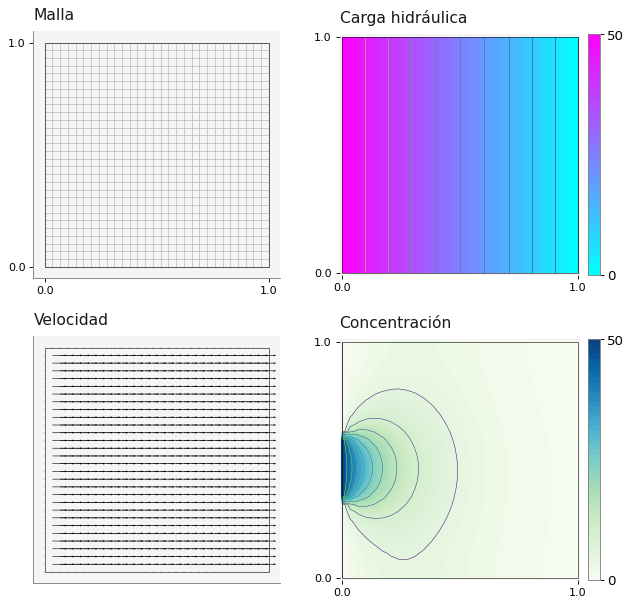
\includegraphics{03_Sol_Sis_Lin_Krylov_files/figure-pdf/cell-20-output-1.png}

\begin{Shaded}
\begin{Highlighting}[]
\CommentTok{\# Lista con el número de las iteraciones}
\NormalTok{l\_itGrad }\OperatorTok{=} \BuiltInTok{list}\NormalTok{(}\BuiltInTok{range}\NormalTok{(}\DecValTok{1}\NormalTok{,itGrad}\OperatorTok{+}\DecValTok{1}\NormalTok{)) }
\NormalTok{l\_itCGM }\OperatorTok{=} \BuiltInTok{list}\NormalTok{(}\BuiltInTok{range}\NormalTok{(}\DecValTok{1}\NormalTok{,itCGM}\OperatorTok{+}\DecValTok{1}\NormalTok{))}

\CommentTok{\# Parámetros para los ejes}
\NormalTok{a\_p }\OperatorTok{=} \BuiltInTok{dict}\NormalTok{(yscale}\OperatorTok{=}\StringTok{\textquotesingle{}log\textquotesingle{}}\NormalTok{, xlabel}\OperatorTok{=}\StringTok{\textquotesingle{}Iteraciones\textquotesingle{}}\NormalTok{, xticks }\OperatorTok{=}\NormalTok{ l\_itGrad)}

\CommentTok{\# Gráfica del error}
\NormalTok{v }\OperatorTok{=}\NormalTok{ mvis.Plotter(}\DecValTok{1}\NormalTok{,}\DecValTok{1}\NormalTok{,[a\_p]) }
\NormalTok{v.axes(}\DecValTok{1}\NormalTok{).set\_title(}\StringTok{\textquotesingle{}Error/Residuo\textquotesingle{}}\NormalTok{, loc}\OperatorTok{=}\StringTok{\textquotesingle{}left\textquotesingle{}}\NormalTok{)}

\NormalTok{v.plot(}\DecValTok{1}\NormalTok{, l\_itGrad, eGrad, marker}\OperatorTok{=}\StringTok{\textquotesingle{}.\textquotesingle{}}\NormalTok{, label}\OperatorTok{=}\StringTok{\textquotesingle{}Error Steepest\textquotesingle{}}\NormalTok{)}
\NormalTok{v.plot(}\DecValTok{1}\NormalTok{, l\_itGrad, rGrad, marker}\OperatorTok{=}\StringTok{\textquotesingle{}.\textquotesingle{}}\NormalTok{, label}\OperatorTok{=}\StringTok{\textquotesingle{}Residuo Steepest\textquotesingle{}}\NormalTok{)}
\NormalTok{v.plot(}\DecValTok{1}\NormalTok{, l\_itCGM, eCGM, marker}\OperatorTok{=}\StringTok{\textquotesingle{}.\textquotesingle{}}\NormalTok{, label}\OperatorTok{=}\StringTok{\textquotesingle{}Error CGM\textquotesingle{}}\NormalTok{)}
\NormalTok{v.plot(}\DecValTok{1}\NormalTok{, l\_itCGM, rCGM, marker}\OperatorTok{=}\StringTok{\textquotesingle{}.\textquotesingle{}}\NormalTok{, label}\OperatorTok{=}\StringTok{\textquotesingle{}Residuo CGM\textquotesingle{}}\NormalTok{)}

\NormalTok{v.legend()}
\NormalTok{v.grid()}
\end{Highlighting}
\end{Shaded}

\includegraphics{03_Sol_Sis_Lin_Krylov_files/figure-pdf/cell-21-output-1.png}

\section{\texorpdfstring{\textbf{Ejercicio
3.}}{Ejercicio 3.}}\label{ejercicio-3.-1}

Carga los archivos \texttt{errorJacobi.npy},
\texttt{errorGaussSeidel.npy} y \texttt{errorSOR.npy} en las variables
\texttt{eJ}, \texttt{eG} y \texttt{eSOR} respectivamente (utiliza la
función \texttt{np.load()}). Posteriormente grafica los errores de los 5
métodos: Jacobi, Gauss-Seidel, SOR, Steepest Descend, CGM. ¿Cuál de
todos estos métodos usarías?

\begin{Shaded}
\begin{Highlighting}[]
\NormalTok{eJ }\OperatorTok{=}\NormalTok{ np.load(}\StringTok{\textquotesingle{}errorJacobi.npy\textquotesingle{}}\NormalTok{)}
\NormalTok{eG }\OperatorTok{=}\NormalTok{ np.load(}\StringTok{\textquotesingle{}errorGaussSeidel.npy\textquotesingle{}}\NormalTok{)}
\NormalTok{eSOR }\OperatorTok{=}\NormalTok{ np.load(}\StringTok{\textquotesingle{}errorSOR.npy\textquotesingle{}}\NormalTok{)}

\CommentTok{\# Lista con el número de las iteraciones}
\NormalTok{l\_itJ }\OperatorTok{=} \BuiltInTok{list}\NormalTok{(}\BuiltInTok{range}\NormalTok{(}\DecValTok{1}\NormalTok{,}\BuiltInTok{len}\NormalTok{(eJ)}\OperatorTok{+}\DecValTok{1}\NormalTok{)) }
\NormalTok{l\_itG }\OperatorTok{=} \BuiltInTok{list}\NormalTok{(}\BuiltInTok{range}\NormalTok{(}\DecValTok{1}\NormalTok{,}\BuiltInTok{len}\NormalTok{(eG)}\OperatorTok{+}\DecValTok{1}\NormalTok{)) }
\NormalTok{l\_itSOR }\OperatorTok{=} \BuiltInTok{list}\NormalTok{(}\BuiltInTok{range}\NormalTok{(}\DecValTok{1}\NormalTok{,}\BuiltInTok{len}\NormalTok{(eSOR)}\OperatorTok{+}\DecValTok{1}\NormalTok{)) }
\NormalTok{l\_itGrad }\OperatorTok{=} \BuiltInTok{list}\NormalTok{(}\BuiltInTok{range}\NormalTok{(}\DecValTok{1}\NormalTok{,itGrad}\OperatorTok{+}\DecValTok{1}\NormalTok{)) }
\NormalTok{l\_itCGM }\OperatorTok{=} \BuiltInTok{list}\NormalTok{(}\BuiltInTok{range}\NormalTok{(}\DecValTok{1}\NormalTok{,itCGM}\OperatorTok{+}\DecValTok{1}\NormalTok{))}

\CommentTok{\# Parámetros para los ejes}
\NormalTok{a\_p }\OperatorTok{=} \BuiltInTok{dict}\NormalTok{(yscale}\OperatorTok{=}\StringTok{\textquotesingle{}log\textquotesingle{}}\NormalTok{, xlabel}\OperatorTok{=}\StringTok{\textquotesingle{}Iteraciones\textquotesingle{}}\NormalTok{, xticks }\OperatorTok{=}\NormalTok{ l\_itGrad)}

\CommentTok{\# Gráfica del error}
\NormalTok{v }\OperatorTok{=}\NormalTok{ mvis.Plotter(}\DecValTok{1}\NormalTok{,}\DecValTok{1}\NormalTok{,[a\_p]) }
\NormalTok{v.axes(}\DecValTok{1}\NormalTok{).set\_title(}\StringTok{\textquotesingle{}Error\textquotesingle{}}\NormalTok{, loc}\OperatorTok{=}\StringTok{\textquotesingle{}left\textquotesingle{}}\NormalTok{)}
\NormalTok{v.plot(}\DecValTok{1}\NormalTok{, l\_itJ, eJ, marker}\OperatorTok{=}\StringTok{\textquotesingle{}.\textquotesingle{}}\NormalTok{, label}\OperatorTok{=}\StringTok{\textquotesingle{}Jacobi\textquotesingle{}}\NormalTok{)}
\NormalTok{v.plot(}\DecValTok{1}\NormalTok{, l\_itG, eG, marker}\OperatorTok{=}\StringTok{\textquotesingle{}.\textquotesingle{}}\NormalTok{, label}\OperatorTok{=}\StringTok{\textquotesingle{}Gauss{-}Seidel\textquotesingle{}}\NormalTok{)}
\NormalTok{v.plot(}\DecValTok{1}\NormalTok{, l\_itSOR, eSOR, marker}\OperatorTok{=}\StringTok{\textquotesingle{}.\textquotesingle{}}\NormalTok{, label}\OperatorTok{=}\StringTok{\textquotesingle{}SOR\textquotesingle{}}\NormalTok{)}
\NormalTok{v.plot(}\DecValTok{1}\NormalTok{, l\_itGrad, eGrad, marker}\OperatorTok{=}\StringTok{\textquotesingle{}.\textquotesingle{}}\NormalTok{, label}\OperatorTok{=}\StringTok{\textquotesingle{}Steepest descend\textquotesingle{}}\NormalTok{)}
\NormalTok{v.plot(}\DecValTok{1}\NormalTok{, l\_itCGM, eCGM, marker}\OperatorTok{=}\StringTok{\textquotesingle{}.\textquotesingle{}}\NormalTok{, label}\OperatorTok{=}\StringTok{\textquotesingle{}Gradiente Conjugado\textquotesingle{}}\NormalTok{)}

\NormalTok{v.legend()}
\NormalTok{v.grid()}
\end{Highlighting}
\end{Shaded}

\includegraphics{03_Sol_Sis_Lin_Krylov_files/figure-pdf/cell-22-output-1.png}

\bookmarksetup{startatroot}

\chapter{Conducción de Calor estaionaria en
2D.}\label{conducciuxf3n-de-calor-estaionaria-en-2d.}

\textbf{Objetivo General} - Resolver numérica y computacionalmente la
ecuación de conducción de calor estacionaria en dos dimensiones usando
un método implícito.

\textbf{Objetivos particulares} - Definir los parámetros físicos y
numéricos. - Definir la malla del dominio. - Definir la temperatura
inicial junto con sus condiciones de frontera y graficarla sobre la
malla. - Definir el sistema lineal y resolverlo. - Graficar la solución.

HeCompA - 02\_cond\_calor by Luis M. de la Cruz is licensed under
Attribution-ShareAlike 4.0 International

\textbf{Trabajo realizado con el apoyo del Programa UNAM-DGAPA-PAPIME
PE101922}

\section{Introducción.}\label{introducciuxf3n.}

\textbf{Jean-Baptiste Joseph Fourier} fue un matemático y físico francés
que ejerció una fuerte influencia en la ciencia a través de su trabajo
\emph{Théorie analytique de la chaleur}. En este trabajo mostró que es
posible analizar la conducción de calor en cuerpos sólidos en términos
de series matemáticas infinitas, las cuales ahora llevan su nombre:
\emph{Series de Fourier}. Fourier comenzó su trabajo en 1807, en
Grenoble, y lo completó en París en 1822. Su trabajo le permitió
expresar la conducción de calor en objetos bidimensionales (hojas muy
delgadas de algún material) en términos de una ecuación diferencial:

\[
\dfrac{\partial T}{ \partial t} = \kappa \left(\dfrac{\partial^2 T}{ \partial x^2} + \dfrac{\partial^2 T}{ \partial y^2}\right) + S
\]

donde \(u\) representa la temperatura en un instante de tiempo \(t\) y
en un punto \((x,y)\) del plano Cartesiano, \(\kappa\) es la
conductividad del material y \(S\) una fuente de calor.

\section{Conducción estacionaria en
2D.}\label{conducciuxf3n-estacionaria-en-2d.}

Cuando el problema es estacionario, es decir no hay cambios en el
tiempo, y el dominio de estudio es una placa en dos dimensiones, como la
que se muestra en la figura, podemos escribir el problema como sigue:

\[
- \kappa \left(\dfrac{\partial^2 T}{ \partial x^2} + \dfrac{\partial^2 T}{ \partial y^2}\right) = S \tag{1}
\] Podemos aplicar condiciones de frontera son de tipo Dirichlet o
Neumann en las paredes de la placa. En la figura se distingue
\(T_L, T_R, T_T\) y \(T_B\) que corresponden a las temperaturas dadas en
las paredes izquierda (LEFT), derecha (RIGHT), arriba (TOP) y abajo
(BOTTOM), respectivamente.

A la ecuación \((1)\) le podemos aplicar el método de diferencias
finitas:

\(\Longrightarrow\)

\[
\begin{eqnarray}
    \frac{\partial^2 T}{\partial x^2}\Big|_{i,j} \approx \frac{T_{i+1,j} - 2 T_{i,j} + T_{i-1,j}}{h_x^2}; \\
    \frac{\partial^2 T}{\partial y^2}\Big|_{i,j} \approx \frac{T_{i,j+1} - 2 T_{i,j} + T_{i,j-1}}{h_y^2}.
\end{eqnarray}
\]\\

de tal manera que obtendríamos un sistema de ecuaciones lineales como el
siguiente:

En general un sistema de ecuaciones lineales puede contener \(n\)
ecuaciones con \(n\) incógnitas y se ve como sigue:

\[
A \cdot \mathbf{x} = \mathbf{b} \Longrightarrow
\left[
\begin{array}{ccccc}
a_{00} & a_{01} & a_{02} & \dots & a_{0n} \\
a_{10} & a_{11} & a_{12} & \dots & a_{1n} \\
\vdots & \vdots & \vdots & \ddots & \vdots \\
a_{n1} & a_{n1} & a_{n2} & \dots & a_{nn}
\end{array} \right] 
\left[
\begin{array}{cccc}
x_{0} \\ x_{1} \\ \vdots \\ x_{n}
\end{array} \right] 
=
\left[
\begin{array}{c}
b_0 \\ b_1 \\ \vdots \\ b_{n}
\end{array}
\right]
\]

El sistema se puede resolver usando diferentes tipos de métodos.

\begin{Shaded}
\begin{Highlighting}[]
\ImportTok{import}\NormalTok{ numpy }\ImportTok{as}\NormalTok{ np}
\ImportTok{import}\NormalTok{ matplotlib.pyplot }\ImportTok{as}\NormalTok{ plt}
\ImportTok{import}\NormalTok{ macti.visual }\ImportTok{as}\NormalTok{ mvis}
\end{Highlighting}
\end{Shaded}

\section{Parámetros físicos y
numéricos}\label{paruxe1metros-fuxedsicos-y-numuxe9ricos}

\begin{Shaded}
\begin{Highlighting}[]
\CommentTok{\# Tamaño del dominio}
\NormalTok{Lx }\OperatorTok{=} \FloatTok{1.0}
\NormalTok{Ly }\OperatorTok{=} \FloatTok{1.0}
\NormalTok{k }\OperatorTok{=} \FloatTok{1.0}
\CommentTok{\# Número de nodos en cada eje}
\NormalTok{Nx }\OperatorTok{=} \DecValTok{4}
\NormalTok{Ny }\OperatorTok{=} \DecValTok{4}

\CommentTok{\# Número total de nodos en cada eje incluyendo las fronteras}
\NormalTok{NxT }\OperatorTok{=}\NormalTok{ Nx }\OperatorTok{+} \DecValTok{2}
\NormalTok{NyT }\OperatorTok{=}\NormalTok{ Ny }\OperatorTok{+} \DecValTok{2}

\CommentTok{\# Número total de nodos}
\NormalTok{NT }\OperatorTok{=}\NormalTok{ NxT }\OperatorTok{*}\NormalTok{ NyT}

\CommentTok{\# Número total de incógnitas}
\NormalTok{N }\OperatorTok{=}\NormalTok{ Nx }\OperatorTok{*}\NormalTok{ Ny}

\CommentTok{\# Tamaño de la malla en cada dirección}
\NormalTok{hx }\OperatorTok{=}\NormalTok{ Lx }\OperatorTok{/}\NormalTok{ (Nx}\OperatorTok{+}\DecValTok{1}\NormalTok{)}
\NormalTok{hy }\OperatorTok{=}\NormalTok{ Ly }\OperatorTok{/}\NormalTok{ (Ny}\OperatorTok{+}\DecValTok{1}\NormalTok{)}

\CommentTok{\# Coordenadas de la malla}
\NormalTok{xn }\OperatorTok{=}\NormalTok{ np.linspace(}\DecValTok{0}\NormalTok{,Lx,NxT)}
\NormalTok{yn }\OperatorTok{=}\NormalTok{ np.linspace(}\DecValTok{0}\NormalTok{,Ly,NyT)}

\CommentTok{\# Generación de una rejilla}
\NormalTok{xg, yg }\OperatorTok{=}\NormalTok{ np.meshgrid(xn, yn, indexing}\OperatorTok{=}\StringTok{\textquotesingle{}ij\textquotesingle{}}\NormalTok{)}
\end{Highlighting}
\end{Shaded}

\begin{Shaded}
\begin{Highlighting}[]
\BuiltInTok{print}\NormalTok{(}\StringTok{\textquotesingle{}Total de nodos en x = }\SpecialCharTok{\{\}}\StringTok{, en y = }\SpecialCharTok{\{\}}\StringTok{\textquotesingle{}}\NormalTok{.}\BuiltInTok{format}\NormalTok{(NxT, NyT))}
\BuiltInTok{print}\NormalTok{(}\StringTok{\textquotesingle{}Total de incógnitas = }\SpecialCharTok{\{\}}\StringTok{\textquotesingle{}}\NormalTok{.}\BuiltInTok{format}\NormalTok{(N))}
\BuiltInTok{print}\NormalTok{(}\StringTok{\textquotesingle{}Coordenadas en x : }\SpecialCharTok{\{\}}\StringTok{\textquotesingle{}}\NormalTok{.}\BuiltInTok{format}\NormalTok{(xn))}
\BuiltInTok{print}\NormalTok{(}\StringTok{\textquotesingle{}Coordenadas en y : }\SpecialCharTok{\{\}}\StringTok{\textquotesingle{}}\NormalTok{.}\BuiltInTok{format}\NormalTok{(yn))}
\BuiltInTok{print}\NormalTok{(}\StringTok{\textquotesingle{}hx = }\SpecialCharTok{\{\}}\StringTok{, hy = }\SpecialCharTok{\{\}}\StringTok{\textquotesingle{}}\NormalTok{.}\BuiltInTok{format}\NormalTok{(hx, hy))}
\end{Highlighting}
\end{Shaded}

\begin{verbatim}
Total de nodos en x = 6, en y = 6
Total de incógnitas = 16
Coordenadas en x : [0.  0.2 0.4 0.6 0.8 1. ]
Coordenadas en y : [0.  0.2 0.4 0.6 0.8 1. ]
hx = 0.2, hy = 0.2
\end{verbatim}

\subsection{Graficación de la malla del
dominio}\label{graficaciuxf3n-de-la-malla-del-dominio}

\begin{Shaded}
\begin{Highlighting}[]
\ImportTok{from}\NormalTok{ mpl\_toolkits.axes\_grid1 }\ImportTok{import}\NormalTok{ make\_axes\_locatable}
\KeywordTok{def}\NormalTok{ set\_axes(ax):}
    \CommentTok{"""}
\CommentTok{    Configura la razón de aspecto, quita las marcas de los ejes y el marco.}
\CommentTok{    }
\CommentTok{    Parameters}
\CommentTok{    {-}{-}{-}{-}{-}{-}{-}{-}{-}{-}}
\CommentTok{    ax: axis}
\CommentTok{    Ejes que se van a configurar.}
\CommentTok{    """}
\NormalTok{    ax.set\_aspect(}\StringTok{\textquotesingle{}equal\textquotesingle{}}\NormalTok{) }
\NormalTok{    ax.set\_xticks([])}
\NormalTok{    ax.set\_yticks([])}
\NormalTok{    ax.spines[}\StringTok{\textquotesingle{}bottom\textquotesingle{}}\NormalTok{].set\_visible(}\VariableTok{False}\NormalTok{)}
\NormalTok{    ax.spines[}\StringTok{\textquotesingle{}left\textquotesingle{}}\NormalTok{].set\_visible(}\VariableTok{False}\NormalTok{)}
    
\KeywordTok{def}\NormalTok{ plot\_mesh(ax, xg, yg):}
    \CommentTok{"""}
\CommentTok{    Dibuja la malla del dominio.}
\CommentTok{    }
\CommentTok{    Paramters}
\CommentTok{    {-}{-}{-}{-}{-}{-}{-}{-}{-}}
\CommentTok{    ax: axis}
\CommentTok{    Son los ejes donde se dibujará la malla.}
\CommentTok{    }
\CommentTok{    xn: np.array}
\CommentTok{    Coordenadas en x de la malla.}
\CommentTok{    }
\CommentTok{    yn: np.array}
\CommentTok{    Coordenadas en y de la malla.}
\CommentTok{    """}
\NormalTok{    set\_axes(ax)}
    
\NormalTok{    xn }\OperatorTok{=}\NormalTok{ xg[:,}\DecValTok{0}\NormalTok{]}
\NormalTok{    yn }\OperatorTok{=}\NormalTok{ yg[}\DecValTok{0}\NormalTok{,:]}
    
    \ControlFlowTok{for}\NormalTok{ xi }\KeywordTok{in}\NormalTok{ xn:}
\NormalTok{        ax.vlines(xi, ymin}\OperatorTok{=}\NormalTok{yn[}\DecValTok{0}\NormalTok{], ymax}\OperatorTok{=}\NormalTok{yn[}\OperatorTok{{-}}\DecValTok{1}\NormalTok{], lw}\OperatorTok{=}\FloatTok{0.5}\NormalTok{, color}\OperatorTok{=}\StringTok{\textquotesingle{}darkgray\textquotesingle{}}\NormalTok{)}
        
    \ControlFlowTok{for}\NormalTok{ yi }\KeywordTok{in}\NormalTok{ yn:}
\NormalTok{        ax.hlines(yi, xmin}\OperatorTok{=}\NormalTok{xn[}\DecValTok{0}\NormalTok{], xmax}\OperatorTok{=}\NormalTok{xn[}\OperatorTok{{-}}\DecValTok{1}\NormalTok{], lw}\OperatorTok{=}\FloatTok{0.5}\NormalTok{, color}\OperatorTok{=}\StringTok{\textquotesingle{}darkgray\textquotesingle{}}\NormalTok{)}
        
\NormalTok{    ax.scatter(xg,yg, marker}\OperatorTok{=}\StringTok{\textquotesingle{}.\textquotesingle{}}\NormalTok{, color}\OperatorTok{=}\StringTok{\textquotesingle{}darkgray\textquotesingle{}}\NormalTok{)}
    
\KeywordTok{def}\NormalTok{ plot\_frame(ax, xn, yn, lw }\OperatorTok{=} \FloatTok{0.5}\NormalTok{, color }\OperatorTok{=} \StringTok{\textquotesingle{}k\textquotesingle{}}\NormalTok{):}
    \CommentTok{"""}
\CommentTok{    Dibuja el recuadro de la malla.}
\CommentTok{    }
\CommentTok{    Paramters}
\CommentTok{    {-}{-}{-}{-}{-}{-}{-}{-}{-}}
\CommentTok{    ax: axis}
\CommentTok{    Son los ejes donde se dibujará la malla.}
\CommentTok{    }
\CommentTok{    xn: np.array}
\CommentTok{    Coordenadas en x de la malla.}
\CommentTok{    }
\CommentTok{    yn: np.array}
\CommentTok{    Coordenadas en y de la malla.}
\CommentTok{    """}
\NormalTok{    set\_axes(ax)}
    
    \CommentTok{\# Dibujamos dos líneas verticales}
\NormalTok{    ax.vlines(xn[}\DecValTok{0}\NormalTok{], ymin}\OperatorTok{=}\NormalTok{yn[}\DecValTok{0}\NormalTok{], ymax}\OperatorTok{=}\NormalTok{yn[}\OperatorTok{{-}}\DecValTok{1}\NormalTok{], lw }\OperatorTok{=}\NormalTok{ lw, color}\OperatorTok{=}\NormalTok{color)}
\NormalTok{    ax.vlines(xn[}\OperatorTok{{-}}\DecValTok{1}\NormalTok{], ymin}\OperatorTok{=}\NormalTok{yn[}\DecValTok{0}\NormalTok{], ymax}\OperatorTok{=}\NormalTok{yn[}\OperatorTok{{-}}\DecValTok{1}\NormalTok{], lw }\OperatorTok{=}\NormalTok{ lw, color}\OperatorTok{=}\NormalTok{color)}

    \CommentTok{\# Dibujamos dos líneas horizontales}
\NormalTok{    ax.hlines(yn[}\DecValTok{0}\NormalTok{], xmin}\OperatorTok{=}\NormalTok{xn[}\DecValTok{0}\NormalTok{], xmax}\OperatorTok{=}\NormalTok{xn[}\OperatorTok{{-}}\DecValTok{1}\NormalTok{], lw }\OperatorTok{=}\NormalTok{ lw, color}\OperatorTok{=}\NormalTok{color)}
\NormalTok{    ax.hlines(yn[}\OperatorTok{{-}}\DecValTok{1}\NormalTok{], xmin}\OperatorTok{=}\NormalTok{xn[}\DecValTok{0}\NormalTok{], xmax}\OperatorTok{=}\NormalTok{xn[}\OperatorTok{{-}}\DecValTok{1}\NormalTok{], lw }\OperatorTok{=}\NormalTok{ lw, color}\OperatorTok{=}\NormalTok{color)}

\KeywordTok{def}\NormalTok{ set\_canvas(ax, Lx, Ly):}
    \CommentTok{"""}
\CommentTok{    Configura un lienzo para hacer las gráficas más estéticas.}
\CommentTok{    }
\CommentTok{    Parameters}
\CommentTok{    {-}{-}{-}{-}{-}{-}{-}{-}{-}{-}}
\CommentTok{    ax: axis}
\CommentTok{    Son los ejes que se van a configurar.}
\CommentTok{    }
\CommentTok{    Lx: float}
\CommentTok{    Tamaño del dominio en dirección x.}
\CommentTok{    }
\CommentTok{    Ly: float}
\CommentTok{    Tamaño del dominio en dirección y.}
\CommentTok{    }
\CommentTok{    Returns}
\CommentTok{    {-}{-}{-}{-}{-}{-}{-}}
\CommentTok{    cax: axis}
\CommentTok{    Eje donde se dibuja el mapa de color.}
\CommentTok{    """}
\NormalTok{    set\_axes(ax)}

\NormalTok{    lmax }\OperatorTok{=} \BuiltInTok{max}\NormalTok{(Lx,Ly)}
\NormalTok{    offx }\OperatorTok{=}\NormalTok{ lmax }\OperatorTok{*} \FloatTok{0.01}
\NormalTok{    offy }\OperatorTok{=}\NormalTok{ lmax }\OperatorTok{*} \FloatTok{0.01}
\NormalTok{    ax.set\_xlim(}\OperatorTok{{-}}\NormalTok{offx, Lx}\OperatorTok{+}\NormalTok{offx)}
\NormalTok{    ax.set\_ylim(}\OperatorTok{{-}}\NormalTok{offy, Ly}\OperatorTok{+}\NormalTok{offy)}
\NormalTok{    ax.grid(}\VariableTok{False}\NormalTok{)}
    
\NormalTok{    ax.set\_aspect(}\StringTok{\textquotesingle{}equal\textquotesingle{}}\NormalTok{)}
\NormalTok{    divider }\OperatorTok{=}\NormalTok{ make\_axes\_locatable(ax)}
\NormalTok{    cax }\OperatorTok{=}\NormalTok{ divider.append\_axes(}\StringTok{"right"}\NormalTok{, }\StringTok{"5\%"}\NormalTok{, pad}\OperatorTok{=}\StringTok{"3\%"}\NormalTok{)}
\NormalTok{    cax.set\_xticks([])}
\NormalTok{    cax.set\_yticks([])}
\NormalTok{    cax.spines[}\StringTok{\textquotesingle{}bottom\textquotesingle{}}\NormalTok{].set\_visible(}\VariableTok{False}\NormalTok{)}
\NormalTok{    cax.spines[}\StringTok{\textquotesingle{}left\textquotesingle{}}\NormalTok{].set\_visible(}\VariableTok{False}\NormalTok{)}
    
    \ControlFlowTok{return}\NormalTok{ cax}
\end{Highlighting}
\end{Shaded}

\begin{Shaded}
\begin{Highlighting}[]
\NormalTok{fig }\OperatorTok{=}\NormalTok{ plt.figure()}
\NormalTok{ax }\OperatorTok{=}\NormalTok{ plt.gca()}

\CommentTok{\# Ejecutamos la función plot\_mesh(...)}
\NormalTok{plot\_mesh(ax, xg, yg)}

\CommentTok{\# Dibujamos el recuadro con la función plot\_fame(...)}
\NormalTok{plot\_frame(ax, xn, yn)}
\end{Highlighting}
\end{Shaded}

\includegraphics{04_Conduccion_estacionaria_files/figure-pdf/cell-6-output-1.png}

\begin{Shaded}
\begin{Highlighting}[]
\NormalTok{vis }\OperatorTok{=}\NormalTok{ mvis.Plotter(}\DecValTok{1}\NormalTok{,}\DecValTok{1}\NormalTok{)}

\NormalTok{vis.draw\_domain(}\DecValTok{1}\NormalTok{, xg, yg)}
\end{Highlighting}
\end{Shaded}

\includegraphics{04_Conduccion_estacionaria_files/figure-pdf/cell-7-output-1.png}

\begin{Shaded}
\begin{Highlighting}[]
\NormalTok{vis }\OperatorTok{=}\NormalTok{ mvis.Plotter(}\DecValTok{1}\NormalTok{,}\DecValTok{2}\NormalTok{,[}\BuiltInTok{dict}\NormalTok{(aspect}\OperatorTok{=}\StringTok{\textquotesingle{}equal\textquotesingle{}}\NormalTok{), }\BuiltInTok{dict}\NormalTok{(aspect}\OperatorTok{=}\StringTok{\textquotesingle{}equal\textquotesingle{}}\NormalTok{)])}

\NormalTok{vis.draw\_domain(}\DecValTok{1}\NormalTok{, xg, yg)}
\NormalTok{vis.plot\_mesh2D(}\DecValTok{2}\NormalTok{, xg, yg)}
\NormalTok{vis.plot\_frame(}\DecValTok{2}\NormalTok{, xg, yg)}
\end{Highlighting}
\end{Shaded}

\includegraphics{04_Conduccion_estacionaria_files/figure-pdf/cell-8-output-1.png}

\section{Campo de temperaturas y sus condiciones de
frontera}\label{campo-de-temperaturas-y-sus-condiciones-de-frontera}

\begin{Shaded}
\begin{Highlighting}[]
\CommentTok{\# Definición de un campo escalar en cada punto de la malla}
\NormalTok{T }\OperatorTok{=}\NormalTok{ np.zeros((NxT, NyT))}

\CommentTok{\# Condiciones de frontera}
\NormalTok{TB }\OperatorTok{=} \FloatTok{1.0}
\NormalTok{TT }\OperatorTok{=} \OperatorTok{{-}}\FloatTok{1.0}

\NormalTok{T[}\DecValTok{0}\NormalTok{ , :] }\OperatorTok{=} \FloatTok{0.0} \CommentTok{\# LEFT}
\NormalTok{T[}\OperatorTok{{-}}\DecValTok{1}\NormalTok{, :] }\OperatorTok{=} \FloatTok{0.0} \CommentTok{\# RIGHT}
\NormalTok{T[: , }\DecValTok{0}\NormalTok{] }\OperatorTok{=}\NormalTok{ TB  }\CommentTok{\# BOTTOM}
\NormalTok{T[: ,}\OperatorTok{{-}}\DecValTok{1}\NormalTok{] }\OperatorTok{=}\NormalTok{ TT  }\CommentTok{\# TOP}

\BuiltInTok{print}\NormalTok{(}\StringTok{\textquotesingle{}Campo escalar T (}\SpecialCharTok{\{\}}\StringTok{):}\CharTok{\textbackslash{}n}\StringTok{ }\SpecialCharTok{\{\}}\StringTok{\textquotesingle{}}\NormalTok{.}\BuiltInTok{format}\NormalTok{(T.shape, T))}
\end{Highlighting}
\end{Shaded}

\begin{verbatim}
Campo escalar T ((6, 6)):
 [[ 1.  0.  0.  0.  0. -1.]
 [ 1.  0.  0.  0.  0. -1.]
 [ 1.  0.  0.  0.  0. -1.]
 [ 1.  0.  0.  0.  0. -1.]
 [ 1.  0.  0.  0.  0. -1.]
 [ 1.  0.  0.  0.  0. -1.]]
\end{verbatim}

\subsection{Graficación del campo escalar sobre la
malla}\label{graficaciuxf3n-del-campo-escalar-sobre-la-malla}

\begin{Shaded}
\begin{Highlighting}[]
\NormalTok{fig }\OperatorTok{=}\NormalTok{ plt.figure()}
\NormalTok{ax }\OperatorTok{=}\NormalTok{ plt.gca()}
\NormalTok{cax }\OperatorTok{=}\NormalTok{ set\_canvas(ax, Lx, Ly)}

\NormalTok{c }\OperatorTok{=}\NormalTok{ ax.contourf(xg, yg, T, levels}\OperatorTok{=}\DecValTok{50}\NormalTok{, cmap}\OperatorTok{=}\StringTok{\textquotesingle{}inferno\textquotesingle{}}\NormalTok{)}
\NormalTok{plot\_mesh(ax, xg, yg)}
\NormalTok{fig.colorbar(c, cax}\OperatorTok{=}\NormalTok{cax, ticks}\OperatorTok{=}\NormalTok{[}\OperatorTok{{-}}\FloatTok{0.9}\NormalTok{, }\FloatTok{0.0}\NormalTok{, }\FloatTok{0.9}\NormalTok{])}
\NormalTok{plt.show()}
\end{Highlighting}
\end{Shaded}

\includegraphics{04_Conduccion_estacionaria_files/figure-pdf/cell-10-output-1.png}

\begin{Shaded}
\begin{Highlighting}[]
\NormalTok{vis }\OperatorTok{=}\NormalTok{ mvis.Plotter(}\DecValTok{1}\NormalTok{,}\DecValTok{3}\NormalTok{,[}\BuiltInTok{dict}\NormalTok{(aspect}\OperatorTok{=}\StringTok{\textquotesingle{}equal\textquotesingle{}}\NormalTok{), }\BuiltInTok{dict}\NormalTok{(aspect}\OperatorTok{=}\StringTok{\textquotesingle{}equal\textquotesingle{}}\NormalTok{), }\BuiltInTok{dict}\NormalTok{(aspect}\OperatorTok{=}\StringTok{\textquotesingle{}equal\textquotesingle{}}\NormalTok{)])}

\NormalTok{vis.draw\_domain(}\DecValTok{1}\NormalTok{, xg, yg)}
\NormalTok{vis.plot\_mesh2D(}\DecValTok{2}\NormalTok{, xg, yg)}
\NormalTok{vis.plot\_frame(}\DecValTok{2}\NormalTok{, xg, yg)}
\NormalTok{vis.contourf(}\DecValTok{3}\NormalTok{, xg, yg, T, levels}\OperatorTok{=}\DecValTok{50}\NormalTok{, cmap}\OperatorTok{=}\StringTok{\textquotesingle{}inferno\textquotesingle{}}\NormalTok{)}
\NormalTok{vis.show()}
\end{Highlighting}
\end{Shaded}

\includegraphics{04_Conduccion_estacionaria_files/figure-pdf/cell-11-output-1.png}

\begin{Shaded}
\begin{Highlighting}[]
\NormalTok{vis }\OperatorTok{=}\NormalTok{ mvis.Plotter(}\DecValTok{1}\NormalTok{,}\DecValTok{3}\NormalTok{,[}\BuiltInTok{dict}\NormalTok{(aspect}\OperatorTok{=}\StringTok{\textquotesingle{}equal\textquotesingle{}}\NormalTok{), }\BuiltInTok{dict}\NormalTok{(aspect}\OperatorTok{=}\StringTok{\textquotesingle{}equal\textquotesingle{}}\NormalTok{), }\BuiltInTok{dict}\NormalTok{(aspect}\OperatorTok{=}\StringTok{\textquotesingle{}equal\textquotesingle{}}\NormalTok{)],}
                  \BuiltInTok{dict}\NormalTok{(figsize}\OperatorTok{=}\NormalTok{(}\DecValTok{8}\NormalTok{,}\DecValTok{16}\NormalTok{)))}

\NormalTok{vis.draw\_domain(}\DecValTok{1}\NormalTok{, xg, yg)}
\NormalTok{vis.plot\_mesh2D(}\DecValTok{2}\NormalTok{, xg, yg, nodeson}\OperatorTok{=}\VariableTok{True}\NormalTok{)}
\NormalTok{vis.plot\_frame(}\DecValTok{2}\NormalTok{, xg, yg)}
\NormalTok{vis.contourf(}\DecValTok{3}\NormalTok{, xg, yg, T, levels}\OperatorTok{=}\DecValTok{50}\NormalTok{, cmap}\OperatorTok{=}\StringTok{\textquotesingle{}inferno\textquotesingle{}}\NormalTok{)}
\NormalTok{vis.plot\_mesh2D(}\DecValTok{3}\NormalTok{,xg, yg)}
\NormalTok{vis.show()}
\end{Highlighting}
\end{Shaded}

\includegraphics{04_Conduccion_estacionaria_files/figure-pdf/cell-12-output-1.png}

\section{Flujo de calor}\label{flujo-de-calor}

Fourier también estableció una ley para el flujo de calor que se escribe
como:

\[
\vec{q} = -\kappa \nabla u = -\kappa \left(\dfrac{\partial u}{\partial x}, \dfrac{\partial u}{\partial y}\right)
\]

\begin{Shaded}
\begin{Highlighting}[]
\KeywordTok{def}\NormalTok{ heat\_flux(T, hx, hy):}
\NormalTok{    NxT, NyT }\OperatorTok{=}\NormalTok{ T.shape}
\NormalTok{    qx }\OperatorTok{=}\NormalTok{ np.zeros(T.shape)}
\NormalTok{    qy }\OperatorTok{=}\NormalTok{ qx.copy()}

    \ControlFlowTok{for}\NormalTok{ i }\KeywordTok{in} \BuiltInTok{range}\NormalTok{(}\DecValTok{1}\NormalTok{,NxT}\OperatorTok{{-}}\DecValTok{1}\NormalTok{):}
        \ControlFlowTok{for}\NormalTok{ j }\KeywordTok{in} \BuiltInTok{range}\NormalTok{(}\DecValTok{1}\NormalTok{,NyT}\OperatorTok{{-}}\DecValTok{1}\NormalTok{):}
\NormalTok{            qx[i,j] }\OperatorTok{=} \OperatorTok{{-}}\NormalTok{k }\OperatorTok{*}\NormalTok{ (T[i}\OperatorTok{+}\DecValTok{1}\NormalTok{,j] }\OperatorTok{{-}}\NormalTok{ T[i}\OperatorTok{{-}}\DecValTok{1}\NormalTok{,j]) }\OperatorTok{/} \DecValTok{2} \OperatorTok{*}\NormalTok{ hx}
\NormalTok{            qy[i,j] }\OperatorTok{=} \OperatorTok{{-}}\NormalTok{k }\OperatorTok{*}\NormalTok{ (T[i,j}\OperatorTok{+}\DecValTok{1}\NormalTok{] }\OperatorTok{{-}}\NormalTok{ T[i,j}\OperatorTok{{-}}\DecValTok{1}\NormalTok{]) }\OperatorTok{/} \DecValTok{2} \OperatorTok{*}\NormalTok{ hy}
    \ControlFlowTok{return}\NormalTok{ qx, qy}
\end{Highlighting}
\end{Shaded}

\begin{Shaded}
\begin{Highlighting}[]
\NormalTok{qx, qy }\OperatorTok{=}\NormalTok{ heat\_flux(T, hx, hy)}
\end{Highlighting}
\end{Shaded}

\begin{Shaded}
\begin{Highlighting}[]
\NormalTok{ax1 }\OperatorTok{=} \BuiltInTok{dict}\NormalTok{(aspect}\OperatorTok{=}\StringTok{\textquotesingle{}equal\textquotesingle{}}\NormalTok{, title}\OperatorTok{=}\StringTok{\textquotesingle{}Dominio\textquotesingle{}}\NormalTok{)}
\NormalTok{ax2 }\OperatorTok{=} \BuiltInTok{dict}\NormalTok{(aspect}\OperatorTok{=}\StringTok{\textquotesingle{}equal\textquotesingle{}}\NormalTok{, title}\OperatorTok{=}\StringTok{\textquotesingle{}Malla\textquotesingle{}}\NormalTok{)}
\NormalTok{ax3 }\OperatorTok{=} \BuiltInTok{dict}\NormalTok{(aspect}\OperatorTok{=}\StringTok{\textquotesingle{}equal\textquotesingle{}}\NormalTok{, title}\OperatorTok{=}\StringTok{\textquotesingle{}Temperatura\textquotesingle{}}\NormalTok{)}
\NormalTok{ax4 }\OperatorTok{=} \BuiltInTok{dict}\NormalTok{(aspect}\OperatorTok{=}\StringTok{\textquotesingle{}equal\textquotesingle{}}\NormalTok{, title}\OperatorTok{=}\StringTok{\textquotesingle{}Flujo de calor\textquotesingle{}}\NormalTok{)}

\NormalTok{vis }\OperatorTok{=}\NormalTok{ mvis.Plotter(}\DecValTok{2}\NormalTok{,}\DecValTok{2}\NormalTok{,[ax1, ax2, ax3, ax4],}
                  \BuiltInTok{dict}\NormalTok{(figsize}\OperatorTok{=}\NormalTok{(}\DecValTok{8}\NormalTok{,}\DecValTok{8}\NormalTok{)))}

\NormalTok{vis.draw\_domain(}\DecValTok{1}\NormalTok{, xg, yg)}
\NormalTok{vis.plot\_mesh2D(}\DecValTok{2}\NormalTok{, xg, yg, nodeson}\OperatorTok{=}\VariableTok{True}\NormalTok{)}
\NormalTok{vis.plot\_frame(}\DecValTok{2}\NormalTok{, xg, yg)}

\NormalTok{cax3 }\OperatorTok{=}\NormalTok{ vis.set\_canvas(}\DecValTok{3}\NormalTok{,Lx,Ly)}
\NormalTok{c }\OperatorTok{=}\NormalTok{ vis.contourf(}\DecValTok{3}\NormalTok{, xg, yg, T, levels}\OperatorTok{=}\DecValTok{50}\NormalTok{, cmap}\OperatorTok{=}\StringTok{\textquotesingle{}inferno\textquotesingle{}}\NormalTok{)}
\NormalTok{vis.fig.colorbar(c, cax}\OperatorTok{=}\NormalTok{cax3, ticks }\OperatorTok{=}\NormalTok{ [T.}\BuiltInTok{min}\NormalTok{(), T.}\BuiltInTok{max}\NormalTok{()], shrink}\OperatorTok{=}\FloatTok{0.5}\NormalTok{, orientation}\OperatorTok{=}\StringTok{\textquotesingle{}vertical\textquotesingle{}}\NormalTok{)}
\NormalTok{vis.plot\_mesh2D(}\DecValTok{3}\NormalTok{, xg, yg)}

\NormalTok{vis.plot\_frame(}\DecValTok{4}\NormalTok{, xg, yg)}
\NormalTok{vis.quiver(}\DecValTok{4}\NormalTok{, xg, yg, qx, qy, scale}\OperatorTok{=}\DecValTok{1}\NormalTok{)}
\NormalTok{vis.show()}
\end{Highlighting}
\end{Shaded}

\includegraphics{04_Conduccion_estacionaria_files/figure-pdf/cell-15-output-1.png}

\section{Sistema lineal}\label{sistema-lineal}

\begin{Shaded}
\begin{Highlighting}[]
\ImportTok{import}\NormalTok{ FDM}
\CommentTok{\# La matriz del sistema. Usamos la función predefinida buildMatrix2D()}
\NormalTok{A }\OperatorTok{=}\NormalTok{ FDM.buildMatrix2D(Nx,Ny,}\OperatorTok{{-}}\DecValTok{4}\NormalTok{)}
\NormalTok{A}
\end{Highlighting}
\end{Shaded}

\begin{verbatim}
array([[-4.,  1.,  0.,  0.,  1.,  0.,  0.,  0.,  0.,  0.,  0.,  0.,  0.,
         0.,  0.,  0.],
       [ 1., -4.,  1.,  0.,  0.,  1.,  0.,  0.,  0.,  0.,  0.,  0.,  0.,
         0.,  0.,  0.],
       [ 0.,  1., -4.,  1.,  0.,  0.,  1.,  0.,  0.,  0.,  0.,  0.,  0.,
         0.,  0.,  0.],
       [ 0.,  0.,  1., -4.,  0.,  0.,  0.,  1.,  0.,  0.,  0.,  0.,  0.,
         0.,  0.,  0.],
       [ 1.,  0.,  0.,  0., -4.,  1.,  0.,  0.,  1.,  0.,  0.,  0.,  0.,
         0.,  0.,  0.],
       [ 0.,  1.,  0.,  0.,  1., -4.,  1.,  0.,  0.,  1.,  0.,  0.,  0.,
         0.,  0.,  0.],
       [ 0.,  0.,  1.,  0.,  0.,  1., -4.,  1.,  0.,  0.,  1.,  0.,  0.,
         0.,  0.,  0.],
       [ 0.,  0.,  0.,  1.,  0.,  0.,  1., -4.,  0.,  0.,  0.,  1.,  0.,
         0.,  0.,  0.],
       [ 0.,  0.,  0.,  0.,  1.,  0.,  0.,  0., -4.,  1.,  0.,  0.,  1.,
         0.,  0.,  0.],
       [ 0.,  0.,  0.,  0.,  0.,  1.,  0.,  0.,  1., -4.,  1.,  0.,  0.,
         1.,  0.,  0.],
       [ 0.,  0.,  0.,  0.,  0.,  0.,  1.,  0.,  0.,  1., -4.,  1.,  0.,
         0.,  1.,  0.],
       [ 0.,  0.,  0.,  0.,  0.,  0.,  0.,  1.,  0.,  0.,  1., -4.,  0.,
         0.,  0.,  1.],
       [ 0.,  0.,  0.,  0.,  0.,  0.,  0.,  0.,  1.,  0.,  0.,  0., -4.,
         1.,  0.,  0.],
       [ 0.,  0.,  0.,  0.,  0.,  0.,  0.,  0.,  0.,  1.,  0.,  0.,  1.,
        -4.,  1.,  0.],
       [ 0.,  0.,  0.,  0.,  0.,  0.,  0.,  0.,  0.,  0.,  1.,  0.,  0.,
         1., -4.,  1.],
       [ 0.,  0.,  0.,  0.,  0.,  0.,  0.,  0.,  0.,  0.,  0.,  1.,  0.,
         0.,  1., -4.]])
\end{verbatim}

\begin{Shaded}
\begin{Highlighting}[]
\CommentTok{\# RHS}
\NormalTok{b }\OperatorTok{=}\NormalTok{ np.zeros((Nx,Ny))}
\NormalTok{b[:, }\DecValTok{0}\NormalTok{] }\OperatorTok{{-}=}\NormalTok{ TB  }\CommentTok{\# BOTTOM}
\NormalTok{b[:,}\OperatorTok{{-}}\DecValTok{1}\NormalTok{] }\OperatorTok{{-}=}\NormalTok{ TT  }\CommentTok{\# TOP}
\NormalTok{b}
\end{Highlighting}
\end{Shaded}

\begin{verbatim}
array([[-1.,  0.,  0.,  1.],
       [-1.,  0.,  0.,  1.],
       [-1.,  0.,  0.,  1.],
       [-1.,  0.,  0.,  1.]])
\end{verbatim}

\section{Solución del sistema}\label{soluciuxf3n-del-sistema}

Revisamos el formato del vector b

\begin{Shaded}
\begin{Highlighting}[]
\NormalTok{b.shape}
\end{Highlighting}
\end{Shaded}

\begin{verbatim}
(4, 4)
\end{verbatim}

El vector debe ser de una sola dimensión:

\begin{Shaded}
\begin{Highlighting}[]
\NormalTok{b.flatten()}
\end{Highlighting}
\end{Shaded}

\begin{verbatim}
array([-1.,  0.,  0.,  1., -1.,  0.,  0.,  1., -1.,  0.,  0.,  1., -1.,
        0.,  0.,  1.])
\end{verbatim}

\begin{Shaded}
\begin{Highlighting}[]
\CommentTok{\# Calculamos la solución.}
\NormalTok{T\_temp }\OperatorTok{=}\NormalTok{ np.linalg.solve(A, b.flatten())}
\NormalTok{T\_temp}
\end{Highlighting}
\end{Shaded}

\begin{verbatim}
array([ 0.40909091,  0.11363636, -0.11363636, -0.40909091,  0.52272727,
        0.15909091, -0.15909091, -0.52272727,  0.52272727,  0.15909091,
       -0.15909091, -0.52272727,  0.40909091,  0.11363636, -0.11363636,
       -0.40909091])
\end{verbatim}

\begin{Shaded}
\begin{Highlighting}[]
\NormalTok{T\_temp.shape}
\end{Highlighting}
\end{Shaded}

\begin{verbatim}
(16,)
\end{verbatim}

Colocamos la solución en el campo escalar T de manera adecuada

\begin{Shaded}
\begin{Highlighting}[]
\NormalTok{T[}\DecValTok{1}\NormalTok{:}\OperatorTok{{-}}\DecValTok{1}\NormalTok{,}\DecValTok{1}\NormalTok{:}\OperatorTok{{-}}\DecValTok{1}\NormalTok{] }\OperatorTok{=}\NormalTok{ T\_temp.reshape(Nx,Ny)}
\NormalTok{T}
\end{Highlighting}
\end{Shaded}

\begin{verbatim}
array([[ 1.        ,  0.        ,  0.        ,  0.        ,  0.        ,
        -1.        ],
       [ 1.        ,  0.40909091,  0.11363636, -0.11363636, -0.40909091,
        -1.        ],
       [ 1.        ,  0.52272727,  0.15909091, -0.15909091, -0.52272727,
        -1.        ],
       [ 1.        ,  0.52272727,  0.15909091, -0.15909091, -0.52272727,
        -1.        ],
       [ 1.        ,  0.40909091,  0.11363636, -0.11363636, -0.40909091,
        -1.        ],
       [ 1.        ,  0.        ,  0.        ,  0.        ,  0.        ,
        -1.        ]])
\end{verbatim}

\begin{Shaded}
\begin{Highlighting}[]
\NormalTok{qx, qy }\OperatorTok{=}\NormalTok{ heat\_flux(T, hx, hy)}
\end{Highlighting}
\end{Shaded}

\subsection{Gráfica de la solución}\label{gruxe1fica-de-la-soluciuxf3n}

\begin{Shaded}
\begin{Highlighting}[]
\NormalTok{vis }\OperatorTok{=}\NormalTok{ mvis.Plotter(}\DecValTok{2}\NormalTok{,}\DecValTok{2}\NormalTok{,[ax1, ax2, ax3, ax4],}
                  \BuiltInTok{dict}\NormalTok{(figsize}\OperatorTok{=}\NormalTok{(}\DecValTok{8}\NormalTok{,}\DecValTok{8}\NormalTok{)))}

\NormalTok{vis.draw\_domain(}\DecValTok{1}\NormalTok{, xg, yg)}
\NormalTok{vis.plot\_mesh2D(}\DecValTok{2}\NormalTok{, xg, yg, nodeson}\OperatorTok{=}\VariableTok{True}\NormalTok{)}
\NormalTok{vis.plot\_frame(}\DecValTok{2}\NormalTok{, xg, yg)}

\NormalTok{cax3 }\OperatorTok{=}\NormalTok{ vis.set\_canvas(}\DecValTok{3}\NormalTok{,Lx,Ly)}
\NormalTok{c }\OperatorTok{=}\NormalTok{ vis.contourf(}\DecValTok{3}\NormalTok{, xg, yg, T, levels}\OperatorTok{=}\DecValTok{50}\NormalTok{, cmap}\OperatorTok{=}\StringTok{\textquotesingle{}inferno\textquotesingle{}}\NormalTok{)}
\NormalTok{vis.fig.colorbar(c, cax}\OperatorTok{=}\NormalTok{cax3, ticks }\OperatorTok{=}\NormalTok{ [T.}\BuiltInTok{min}\NormalTok{(), T.}\BuiltInTok{max}\NormalTok{()], shrink}\OperatorTok{=}\FloatTok{0.5}\NormalTok{, orientation}\OperatorTok{=}\StringTok{\textquotesingle{}vertical\textquotesingle{}}\NormalTok{)}
\NormalTok{vis.plot\_mesh2D(}\DecValTok{3}\NormalTok{, xg, yg)}

\NormalTok{vis.plot\_frame(}\DecValTok{4}\NormalTok{, xg, yg)}
\NormalTok{vis.quiver(}\DecValTok{4}\NormalTok{, xg, yg, qx, qy, scale}\OperatorTok{=}\DecValTok{1}\NormalTok{)}
\NormalTok{vis.show()}
\end{Highlighting}
\end{Shaded}

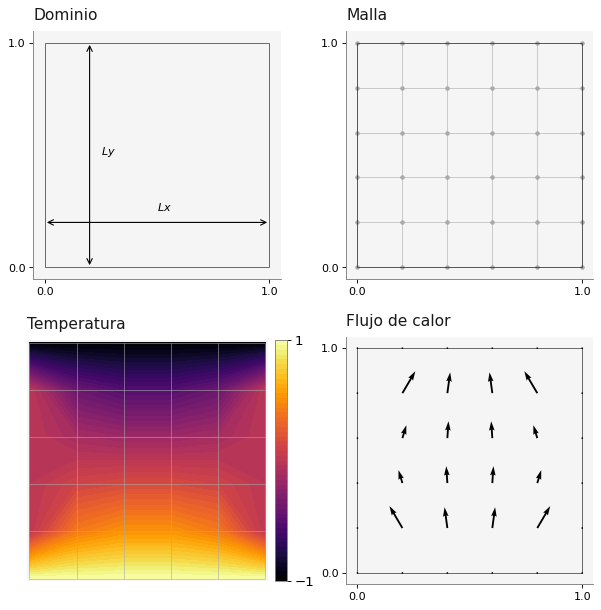
\includegraphics{04_Conduccion_estacionaria_files/figure-pdf/cell-24-output-1.png}

\subsection{Interactivo}\label{interactivo}

\begin{Shaded}
\begin{Highlighting}[]
\KeywordTok{def}\NormalTok{ heat\_cond(Lx, Ly, Nx, Ny):}
    \CommentTok{\# Número total de nodos en cada eje incluyendo las fronteras}
\NormalTok{    NxT }\OperatorTok{=}\NormalTok{ Nx }\OperatorTok{+} \DecValTok{2}
\NormalTok{    NyT }\OperatorTok{=}\NormalTok{ Ny }\OperatorTok{+} \DecValTok{2}
    
    \CommentTok{\# Número total de nodos}
\NormalTok{    NT }\OperatorTok{=}\NormalTok{ NxT }\OperatorTok{*}\NormalTok{ NyT}
    
    \CommentTok{\# Número total de incógnitas}
\NormalTok{    N }\OperatorTok{=}\NormalTok{ Nx }\OperatorTok{*}\NormalTok{ Ny}
    
    \CommentTok{\# Tamaño de la malla en cada dirección}
\NormalTok{    hx }\OperatorTok{=}\NormalTok{ Lx }\OperatorTok{/}\NormalTok{ (Nx}\OperatorTok{+}\DecValTok{1}\NormalTok{)}
\NormalTok{    hy }\OperatorTok{=}\NormalTok{ Ly }\OperatorTok{/}\NormalTok{ (Ny}\OperatorTok{+}\DecValTok{1}\NormalTok{)}
    
    \CommentTok{\# Coordenadas de la malla}
\NormalTok{    xn }\OperatorTok{=}\NormalTok{ np.linspace(}\DecValTok{0}\NormalTok{,Lx,NxT)}
\NormalTok{    yn }\OperatorTok{=}\NormalTok{ np.linspace(}\DecValTok{0}\NormalTok{,Ly,NyT)}
    
    \CommentTok{\# Generación de una rejilla}
\NormalTok{    xg, yg }\OperatorTok{=}\NormalTok{ np.meshgrid(xn, yn, indexing}\OperatorTok{=}\StringTok{\textquotesingle{}ij\textquotesingle{}}\NormalTok{)}

    \CommentTok{\# Definición de un campo escalar en cada punto de la malla}
\NormalTok{    T }\OperatorTok{=}\NormalTok{ np.zeros((NxT, NyT))}
    
    \CommentTok{\# Condiciones de frontera}
\NormalTok{    TB }\OperatorTok{=} \FloatTok{1.0}
\NormalTok{    TT }\OperatorTok{=} \OperatorTok{{-}}\FloatTok{1.0}
    
\NormalTok{    T[}\DecValTok{0}\NormalTok{ , :] }\OperatorTok{=} \FloatTok{0.0} \CommentTok{\# LEFT}
\NormalTok{    T[}\OperatorTok{{-}}\DecValTok{1}\NormalTok{, :] }\OperatorTok{=} \FloatTok{0.0} \CommentTok{\# RIGHT}
\NormalTok{    T[: , }\DecValTok{0}\NormalTok{] }\OperatorTok{=}\NormalTok{ TB  }\CommentTok{\# BOTTOM}
\NormalTok{    T[: ,}\OperatorTok{{-}}\DecValTok{1}\NormalTok{] }\OperatorTok{=}\NormalTok{ TT  }\CommentTok{\# TOP}

    \CommentTok{\# La matriz del sistema. Usamos la función predefinida buildMatrix2D()}
\NormalTok{    A }\OperatorTok{=}\NormalTok{ FDM.buildMatrix2D(Nx,Ny,}\OperatorTok{{-}}\DecValTok{4}\NormalTok{)}

    \CommentTok{\# RHS}
\NormalTok{    b }\OperatorTok{=}\NormalTok{ np.zeros((Nx,Ny))}
\NormalTok{    b[:, }\DecValTok{0}\NormalTok{] }\OperatorTok{{-}=}\NormalTok{ TB  }\CommentTok{\# BOTTOM}
\NormalTok{    b[:,}\OperatorTok{{-}}\DecValTok{1}\NormalTok{] }\OperatorTok{{-}=}\NormalTok{ TT  }\CommentTok{\# TOP}

    \CommentTok{\# Calculamos la solución.}
\NormalTok{    T[}\DecValTok{1}\NormalTok{:}\OperatorTok{{-}}\DecValTok{1}\NormalTok{,}\DecValTok{1}\NormalTok{:}\OperatorTok{{-}}\DecValTok{1}\NormalTok{] }\OperatorTok{=}\NormalTok{ np.linalg.solve(A, b.flatten()).reshape(Nx,Ny)}

    \CommentTok{\# Calculamos el flujo de calor}
\NormalTok{    qx, qy }\OperatorTok{=}\NormalTok{ heat\_flux(T, hx, hy)}

\NormalTok{    ax1 }\OperatorTok{=} \BuiltInTok{dict}\NormalTok{(aspect}\OperatorTok{=}\StringTok{\textquotesingle{}equal\textquotesingle{}}\NormalTok{, title}\OperatorTok{=}\StringTok{\textquotesingle{}Dominio\textquotesingle{}}\NormalTok{)}
\NormalTok{    ax2 }\OperatorTok{=} \BuiltInTok{dict}\NormalTok{(aspect}\OperatorTok{=}\StringTok{\textquotesingle{}equal\textquotesingle{}}\NormalTok{, title}\OperatorTok{=}\StringTok{\textquotesingle{}Malla\textquotesingle{}}\NormalTok{)}
\NormalTok{    ax3 }\OperatorTok{=} \BuiltInTok{dict}\NormalTok{(aspect}\OperatorTok{=}\StringTok{\textquotesingle{}equal\textquotesingle{}}\NormalTok{, title}\OperatorTok{=}\StringTok{\textquotesingle{}Temperatura\textquotesingle{}}\NormalTok{)}
\NormalTok{    ax4 }\OperatorTok{=} \BuiltInTok{dict}\NormalTok{(aspect}\OperatorTok{=}\StringTok{\textquotesingle{}equal\textquotesingle{}}\NormalTok{, title}\OperatorTok{=}\StringTok{\textquotesingle{}Flujo de calor\textquotesingle{}}\NormalTok{)}

\NormalTok{    vis }\OperatorTok{=}\NormalTok{ mvis.Plotter(}\DecValTok{2}\NormalTok{,}\DecValTok{2}\NormalTok{,[ax1, ax2, ax3, ax4],}
                      \BuiltInTok{dict}\NormalTok{(figsize}\OperatorTok{=}\NormalTok{(}\DecValTok{8}\NormalTok{,}\DecValTok{8}\NormalTok{)))}
    
\NormalTok{    vis.draw\_domain(}\DecValTok{1}\NormalTok{, xg, yg)}
\NormalTok{    vis.plot\_mesh2D(}\DecValTok{2}\NormalTok{, xg, yg, nodeson}\OperatorTok{=}\VariableTok{True}\NormalTok{)}
\NormalTok{    vis.plot\_frame(}\DecValTok{2}\NormalTok{, xg, yg)}
    
\NormalTok{    cax3 }\OperatorTok{=}\NormalTok{ vis.set\_canvas(}\DecValTok{3}\NormalTok{,Lx,Ly)}
\NormalTok{    c }\OperatorTok{=}\NormalTok{ vis.contourf(}\DecValTok{3}\NormalTok{, xg, yg, T, levels}\OperatorTok{=}\DecValTok{50}\NormalTok{, cmap}\OperatorTok{=}\StringTok{\textquotesingle{}inferno\textquotesingle{}}\NormalTok{)}
\NormalTok{    vis.fig.colorbar(c, cax}\OperatorTok{=}\NormalTok{cax3, ticks }\OperatorTok{=}\NormalTok{ [T.}\BuiltInTok{min}\NormalTok{(), T.}\BuiltInTok{max}\NormalTok{()], shrink}\OperatorTok{=}\FloatTok{0.5}\NormalTok{, orientation}\OperatorTok{=}\StringTok{\textquotesingle{}vertical\textquotesingle{}}\NormalTok{)}
\NormalTok{    vis.plot\_mesh2D(}\DecValTok{3}\NormalTok{, xg, yg)}
    
\NormalTok{    vis.plot\_frame(}\DecValTok{4}\NormalTok{, xg, yg)}
\NormalTok{    vis.quiver(}\DecValTok{4}\NormalTok{, xg, yg, qx, qy, scale}\OperatorTok{=}\DecValTok{1}\NormalTok{)}
\NormalTok{    vis.show()}
\end{Highlighting}
\end{Shaded}

\begin{Shaded}
\begin{Highlighting}[]
\NormalTok{heat\_cond(Lx}\OperatorTok{=}\DecValTok{1}\NormalTok{, Ly}\OperatorTok{=}\DecValTok{1}\NormalTok{, Nx}\OperatorTok{=}\DecValTok{4}\NormalTok{, Ny}\OperatorTok{=}\DecValTok{4}\NormalTok{)}
\end{Highlighting}
\end{Shaded}

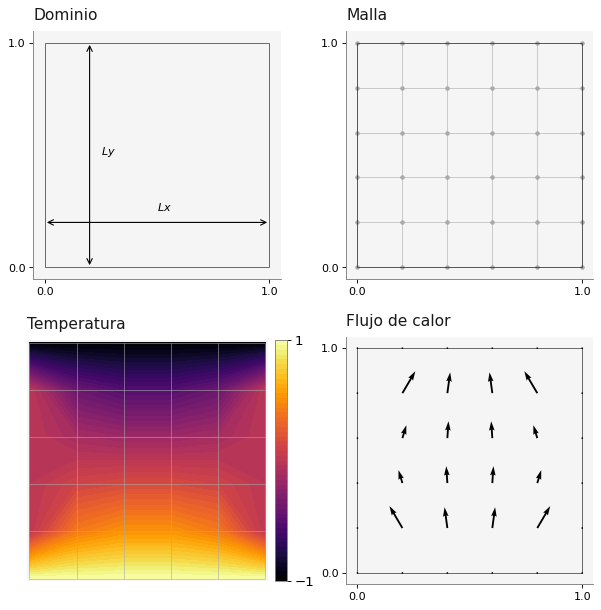
\includegraphics{04_Conduccion_estacionaria_files/figure-pdf/cell-26-output-1.png}

\begin{Shaded}
\begin{Highlighting}[]
\ImportTok{import}\NormalTok{ ipywidgets }\ImportTok{as}\NormalTok{ widgets}
\end{Highlighting}
\end{Shaded}

\begin{Shaded}
\begin{Highlighting}[]
\NormalTok{widgets.interact(heat\_cond, Lx }\OperatorTok{=}\NormalTok{ (}\DecValTok{1}\NormalTok{,}\DecValTok{3}\NormalTok{,}\DecValTok{1}\NormalTok{), Ly }\OperatorTok{=}\NormalTok{ (}\DecValTok{1}\NormalTok{,}\DecValTok{3}\NormalTok{,}\DecValTok{1}\NormalTok{), Nx }\OperatorTok{=}\NormalTok{ (}\DecValTok{4}\NormalTok{, }\DecValTok{8}\NormalTok{, }\DecValTok{1}\NormalTok{), Ny }\OperatorTok{=}\NormalTok{ (}\DecValTok{4}\NormalTok{, }\DecValTok{8}\NormalTok{, }\DecValTok{1}\NormalTok{))}
\end{Highlighting}
\end{Shaded}

\begin{verbatim}
interactive(children=(IntSlider(value=2, description='Lx', max=3, min=1), IntSlider(value=2, description='Ly',…
\end{verbatim}

\begin{verbatim}
<function __main__.heat_cond(Lx, Ly, Nx, Ny)>
\end{verbatim}

\bookmarksetup{startatroot}

\chapter{Conducción de calor No
estacionaria.}\label{conducciuxf3n-de-calor-no-estacionaria.}

\textbf{Objetivo.}

Resolver la ecuación de calor no estacionaria en 2D usando un método
explícito.

HeCompA - 02\_cond\_calor by Luis M. de la Cruz is licensed under
Attribution-ShareAlike 4.0 International

\textbf{Trabajo realizado con el apoyo del Programa UNAM-DGAPA-PAPIME
PE101922}

\bookmarksetup{startatroot}

\chapter{Conducción de calor}\label{conducciuxf3n-de-calor}

\textbf{Jean-Baptiste Joseph Fourier} fue un matemático y físico francés
que ejerció una fuerte influencia en la ciencia a través de su trabajo
\emph{Théorie analytique de la chaleur}. En este trabajo mostró que es
posible analizar la conducción de calor en cuerpos sólidos en términos
de series matemáticas infinitas, las cuales ahora llevan su nombre:
\emph{Series de Fourier}. Fourier comenzó su trabajo en 1807, en
Grenoble, y lo completó en París en 1822. Su trabajo le permitió
expresar la conducción de calor en objetos bidimensionales (hojas muy
delgadas de algún material) en términos de una ecuación diferencial:

\[
\dfrac{\partial u}{ \partial t} = \kappa \left(\dfrac{\partial^2 u}{ \partial x^2} + \dfrac{\partial^2 u}{ \partial y^2}\right)
\]

donde \(u\) representa la temperatura en un instante de tiempo \(t\) y
en un punto \((x,y)\) del plano Cartesiano y \(\kappa\) es la
conductividad del material.

La solución a la ecuación anterior se puede aproximar usando el método
de diferencias y una fórmula explícita de dicha solución es la
siguiente:

\[
u_{i,j}^{n+1} = u_{i,j}^n + \dfrac{h_t\kappa}{h^2} 
\left(u_{i+1,j}^n + u_{i-1,j}^n + u_{i,j+1}^n + u_{i,j-1}^n - 4u_{i,j}^n\right) 
\]

donde: -
\(u_{i,j} = u(x_i, y_j), u_{i+1,j} = u(x_{i+1}, y_j), u_{i-1,j} = u(x_{i-1}, y_j), u_{i,j+1} = u(x_i, y_{j+1}), u_{i,j-1} = u(x_i, y_{j-1})\).
- El superíndice indica el instante de tiempo, entonces el instante
actual es \(n = t\) y el instante siguiente es \(n+1 = t + h_t\), con
\(h_t\) el paso de tiempo. - En este ejemplo \(h_x = h_y\).

Usando esta aproximación, vamos a realizar una ejemplo de conducción de
calor, pero para ello necesitamos conocer las herramientas de numpy y de
matplotlib.

\section{Ejercicio 1.}\label{ejercicio-1.-2}

Calculemos la transferencia de calor por conducción en una placa
cuadrada unitaria usando el método de diferencias finitas. El problema
se describe de la siguiente manera: \[
\dfrac{\partial u}{ \partial t} = \kappa \left(\dfrac{\partial^2 u}{ \partial x^2} + \dfrac{\partial^2 u}{ \partial y^2}\right)
\] \[
\begin{eqnarray}
\hline
u(x,y,t=0) & = & 0 \qquad \text{Condición inicial}\\
\hline
u(0,y,t) & = & 20 \qquad \text{Condiciones}\\
u(1,y,t) & = & 5 \qquad \qquad \text{de}\\
u(x,0,t) & = & 50 \qquad \text{frontera}\\
u(x,1,t) & = & 8 \\
\hline
\end{eqnarray}
\]

\textbf{1. Definir los parámetros físicos y numéricos del problema:}

\begin{Shaded}
\begin{Highlighting}[]
\ImportTok{import}\NormalTok{ numpy }\ImportTok{as}\NormalTok{ np}
\end{Highlighting}
\end{Shaded}

\begin{Shaded}
\begin{Highlighting}[]
\CommentTok{\# Parámetros físicos}
\NormalTok{k }\OperatorTok{=} \FloatTok{1.0}  \CommentTok{\# Conductividad}
\NormalTok{Lx }\OperatorTok{=} \FloatTok{1.0}  \CommentTok{\# Longitud del dominio en dirección x}
\NormalTok{Ly }\OperatorTok{=} \FloatTok{1.0}  \CommentTok{\# Longitud del dominio en dirección y}

\CommentTok{\# Parámetros numéricos}
\NormalTok{Nx }\OperatorTok{=} \DecValTok{9} \CommentTok{\# Número de incógnitas en dirección x}
\NormalTok{Ny }\OperatorTok{=} \DecValTok{9} \CommentTok{\# Número de incógnitas en dirección y}
\NormalTok{h }\OperatorTok{=}\NormalTok{ Lx }\OperatorTok{/}\NormalTok{ (Nx}\OperatorTok{+}\DecValTok{1}\NormalTok{) }\CommentTok{\# Espaciamiento entre los puntos de la rejilla}
\NormalTok{ht }\OperatorTok{=} \FloatTok{0.0001}     \CommentTok{\# Paso de tiempo}
\NormalTok{N }\OperatorTok{=}\NormalTok{ (Nx }\OperatorTok{+} \DecValTok{2}\NormalTok{)}\OperatorTok{*}\NormalTok{ (Ny }\OperatorTok{+} \DecValTok{2}\NormalTok{) }\CommentTok{\# Número total de puntos en la rejilla}
\end{Highlighting}
\end{Shaded}

\textbf{2. Definir la rejilla donde se hará el cálculo (malla):}

\begin{Shaded}
\begin{Highlighting}[]
\NormalTok{x }\OperatorTok{=}\NormalTok{ np.linspace(}\DecValTok{0}\NormalTok{,Lx,Nx}\OperatorTok{+}\DecValTok{2}\NormalTok{) }\CommentTok{\# Arreglo con las coordenadas en x}
\NormalTok{y }\OperatorTok{=}\NormalTok{ np.linspace(}\DecValTok{0}\NormalTok{,Ly,Ny}\OperatorTok{+}\DecValTok{2}\NormalTok{) }\CommentTok{\# Arreglo con las coordenadas en y}
\BuiltInTok{print}\NormalTok{(x)}
\BuiltInTok{print}\NormalTok{(y)}
\end{Highlighting}
\end{Shaded}

\begin{verbatim}
[0.  0.1 0.2 0.3 0.4 0.5 0.6 0.7 0.8 0.9 1. ]
[0.  0.1 0.2 0.3 0.4 0.5 0.6 0.7 0.8 0.9 1. ]
\end{verbatim}

\begin{Shaded}
\begin{Highlighting}[]
\NormalTok{xg, yg }\OperatorTok{=}\NormalTok{ np.meshgrid(x,y) }\CommentTok{\# Creamos la rejilla para usarla en Matplotlib}
\BuiltInTok{print}\NormalTok{(xg)}
\BuiltInTok{print}\NormalTok{(yg)}
\end{Highlighting}
\end{Shaded}

\begin{verbatim}
[[0.  0.1 0.2 0.3 0.4 0.5 0.6 0.7 0.8 0.9 1. ]
 [0.  0.1 0.2 0.3 0.4 0.5 0.6 0.7 0.8 0.9 1. ]
 [0.  0.1 0.2 0.3 0.4 0.5 0.6 0.7 0.8 0.9 1. ]
 [0.  0.1 0.2 0.3 0.4 0.5 0.6 0.7 0.8 0.9 1. ]
 [0.  0.1 0.2 0.3 0.4 0.5 0.6 0.7 0.8 0.9 1. ]
 [0.  0.1 0.2 0.3 0.4 0.5 0.6 0.7 0.8 0.9 1. ]
 [0.  0.1 0.2 0.3 0.4 0.5 0.6 0.7 0.8 0.9 1. ]
 [0.  0.1 0.2 0.3 0.4 0.5 0.6 0.7 0.8 0.9 1. ]
 [0.  0.1 0.2 0.3 0.4 0.5 0.6 0.7 0.8 0.9 1. ]
 [0.  0.1 0.2 0.3 0.4 0.5 0.6 0.7 0.8 0.9 1. ]
 [0.  0.1 0.2 0.3 0.4 0.5 0.6 0.7 0.8 0.9 1. ]]
[[0.  0.  0.  0.  0.  0.  0.  0.  0.  0.  0. ]
 [0.1 0.1 0.1 0.1 0.1 0.1 0.1 0.1 0.1 0.1 0.1]
 [0.2 0.2 0.2 0.2 0.2 0.2 0.2 0.2 0.2 0.2 0.2]
 [0.3 0.3 0.3 0.3 0.3 0.3 0.3 0.3 0.3 0.3 0.3]
 [0.4 0.4 0.4 0.4 0.4 0.4 0.4 0.4 0.4 0.4 0.4]
 [0.5 0.5 0.5 0.5 0.5 0.5 0.5 0.5 0.5 0.5 0.5]
 [0.6 0.6 0.6 0.6 0.6 0.6 0.6 0.6 0.6 0.6 0.6]
 [0.7 0.7 0.7 0.7 0.7 0.7 0.7 0.7 0.7 0.7 0.7]
 [0.8 0.8 0.8 0.8 0.8 0.8 0.8 0.8 0.8 0.8 0.8]
 [0.9 0.9 0.9 0.9 0.9 0.9 0.9 0.9 0.9 0.9 0.9]
 [1.  1.  1.  1.  1.  1.  1.  1.  1.  1.  1. ]]
\end{verbatim}

\begin{Shaded}
\begin{Highlighting}[]
\ImportTok{import}\NormalTok{ matplotlib.pyplot }\ImportTok{as}\NormalTok{ plt}
\end{Highlighting}
\end{Shaded}

\begin{Shaded}
\begin{Highlighting}[]
\NormalTok{plt.scatter(xg, yg) }\CommentTok{\# Graficamos la rejilla}
\end{Highlighting}
\end{Shaded}

\includegraphics{05_Conduccion_NO_estacionaria_files/figure-pdf/cell-7-output-1.png}

\textbf{3. Definir las condiciones iniciales y de frontera:} \[
\begin{eqnarray}
\hline
u(x,y,t=0) & = & 0 \qquad \text{Condición inicial}\\
\hline
u(0,y,t) & = & 20 \qquad \text{Condiciones}\\
u(1,y,t) & = & 5 \qquad \qquad \text{de}\\
u(x,0,t) & = & 50 \qquad \text{frontera}\\
u(x,1,t) & = & 8 \\
\hline
\end{eqnarray}
\]

\begin{Shaded}
\begin{Highlighting}[]
\NormalTok{u }\OperatorTok{=}\NormalTok{ np.zeros((Nx}\OperatorTok{+}\DecValTok{2}\NormalTok{, Ny}\OperatorTok{+}\DecValTok{2}\NormalTok{))}
\CommentTok{\#u = np.zeros(N).reshape(Nx+2, Ny+2) \# Arreglo para almacenar la aproximación}
\BuiltInTok{print}\NormalTok{(u)}
\NormalTok{u[}\DecValTok{0}\NormalTok{,:]    }\OperatorTok{=} \DecValTok{20}  \CommentTok{\# Pared izquierda    }
\NormalTok{u[Nx}\OperatorTok{+}\DecValTok{1}\NormalTok{,:] }\OperatorTok{=} \DecValTok{5}   \CommentTok{\# Pared derecha}
\NormalTok{u[:,}\DecValTok{0}\NormalTok{]    }\OperatorTok{=} \DecValTok{50}  \CommentTok{\# Pared inferior}
\NormalTok{u[:,Ny}\OperatorTok{+}\DecValTok{1}\NormalTok{] }\OperatorTok{=} \DecValTok{8}   \CommentTok{\# Pared superior  }
\BuiltInTok{print}\NormalTok{(u) }
\end{Highlighting}
\end{Shaded}

\begin{verbatim}
[[0. 0. 0. 0. 0. 0. 0. 0. 0. 0. 0.]
 [0. 0. 0. 0. 0. 0. 0. 0. 0. 0. 0.]
 [0. 0. 0. 0. 0. 0. 0. 0. 0. 0. 0.]
 [0. 0. 0. 0. 0. 0. 0. 0. 0. 0. 0.]
 [0. 0. 0. 0. 0. 0. 0. 0. 0. 0. 0.]
 [0. 0. 0. 0. 0. 0. 0. 0. 0. 0. 0.]
 [0. 0. 0. 0. 0. 0. 0. 0. 0. 0. 0.]
 [0. 0. 0. 0. 0. 0. 0. 0. 0. 0. 0.]
 [0. 0. 0. 0. 0. 0. 0. 0. 0. 0. 0.]
 [0. 0. 0. 0. 0. 0. 0. 0. 0. 0. 0.]
 [0. 0. 0. 0. 0. 0. 0. 0. 0. 0. 0.]]
[[50. 20. 20. 20. 20. 20. 20. 20. 20. 20.  8.]
 [50.  0.  0.  0.  0.  0.  0.  0.  0.  0.  8.]
 [50.  0.  0.  0.  0.  0.  0.  0.  0.  0.  8.]
 [50.  0.  0.  0.  0.  0.  0.  0.  0.  0.  8.]
 [50.  0.  0.  0.  0.  0.  0.  0.  0.  0.  8.]
 [50.  0.  0.  0.  0.  0.  0.  0.  0.  0.  8.]
 [50.  0.  0.  0.  0.  0.  0.  0.  0.  0.  8.]
 [50.  0.  0.  0.  0.  0.  0.  0.  0.  0.  8.]
 [50.  0.  0.  0.  0.  0.  0.  0.  0.  0.  8.]
 [50.  0.  0.  0.  0.  0.  0.  0.  0.  0.  8.]
 [50.  5.  5.  5.  5.  5.  5.  5.  5.  5.  8.]]
\end{verbatim}

\begin{Shaded}
\begin{Highlighting}[]
\NormalTok{f }\OperatorTok{=}\NormalTok{ plt.imshow(u)}
\NormalTok{plt.colorbar(f)}
\end{Highlighting}
\end{Shaded}

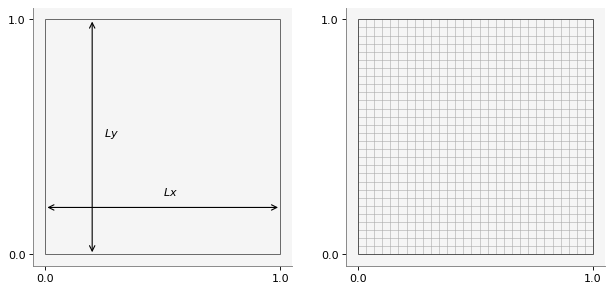
\includegraphics{05_Conduccion_NO_estacionaria_files/figure-pdf/cell-9-output-1.png}

\textbf{4. Implementar el algoritmo de solución:} \[
u_{i,j}^{n+1} = u_{i,j}^n + \dfrac{h_t \kappa}{h^2} 
\left(u_{i+1,j}^n + u_{i-1,j}^n + u_{i,j+1}^n + u_{i,j-1}^n - 4u_{i,j}^n\right) 
\]

\begin{Shaded}
\begin{Highlighting}[]
\NormalTok{ht }\OperatorTok{=} \FloatTok{0.001}
\NormalTok{r }\OperatorTok{=}\NormalTok{ k }\OperatorTok{*}\NormalTok{ ht }\OperatorTok{/}\NormalTok{ h}\OperatorTok{**}\DecValTok{2}
\NormalTok{u\_new }\OperatorTok{=}\NormalTok{ u.copy()}
\NormalTok{tolerancia }\OperatorTok{=} \FloatTok{9.0e{-}1} \CommentTok{\#1.0e{-}3}
\NormalTok{error }\OperatorTok{=} \FloatTok{1.0}
\NormalTok{error\_lista }\OperatorTok{=}\NormalTok{ []}
\ControlFlowTok{while}\NormalTok{(error }\OperatorTok{\textgreater{}}\NormalTok{ tolerancia):}
    \ControlFlowTok{for}\NormalTok{ i }\KeywordTok{in} \BuiltInTok{range}\NormalTok{(}\DecValTok{1}\NormalTok{,Nx}\OperatorTok{+}\DecValTok{1}\NormalTok{):}
        \ControlFlowTok{for}\NormalTok{ j }\KeywordTok{in} \BuiltInTok{range}\NormalTok{(}\DecValTok{1}\NormalTok{,Ny}\OperatorTok{+}\DecValTok{1}\NormalTok{):}
\NormalTok{            u\_new[i,j] }\OperatorTok{=}\NormalTok{ u[i,j] }\OperatorTok{+}\NormalTok{ r }\OperatorTok{*}\NormalTok{ (u[i}\OperatorTok{+}\DecValTok{1}\NormalTok{,j] }\OperatorTok{+}\NormalTok{ u[i}\OperatorTok{{-}}\DecValTok{1}\NormalTok{,j] }\OperatorTok{+}\NormalTok{ u[i,j}\OperatorTok{+}\DecValTok{1}\NormalTok{] }\OperatorTok{+}\NormalTok{ u[i,j}\OperatorTok{{-}}\DecValTok{1}\NormalTok{] }\OperatorTok{{-}} \DecValTok{4}\OperatorTok{*}\NormalTok{u[i,j])}
\NormalTok{    error }\OperatorTok{=}\NormalTok{ np.linalg.norm(u\_new }\OperatorTok{{-}}\NormalTok{ u)}
\NormalTok{    error\_lista.append(error)}
\CommentTok{\#    print(error)}
\NormalTok{    u[:] }\OperatorTok{=}\NormalTok{ u\_new[:]}

\BuiltInTok{print}\NormalTok{(error\_lista)}

\NormalTok{f }\OperatorTok{=}\NormalTok{ plt.imshow(u)}
\NormalTok{plt.colorbar(f)}
\end{Highlighting}
\end{Shaded}

\begin{verbatim}
[17.2629661414254, 13.602554907075358, 11.121464292079526, 9.370340343338656, 8.089431314598079, 7.121431307338295, 6.368158288285477, 5.766710029025608, 5.275727580531657, 4.867291496014421, 4.522054027452314, 4.226261372943586, 3.9698959855402296, 3.745493517737013, 3.547373613271126, 3.3711295389631717, 3.21328287724892, 3.0710454523767496, 2.9421521475712167, 2.824741357872151, 2.7172679513259683, 2.6184387521297463, 2.5271638648303663, 2.4425193146763595, 2.363717902820954, 2.290086125094306, 2.2210456430727876, 2.1560982312045556, 2.094813422134956, 2.0368182790286324, 1.9817888683696612, 1.9294431092766995, 1.8795347490871392, 1.8318482687809046, 1.7861945617665091, 1.7424072597326865, 1.7003396024699928, 1.6598617667041742, 1.620858583384764, 1.5832275844672883, 1.5468773296753073, 1.5117259715044917, 1.4777000231834065, 1.4447332996949114, 1.4127660064863383, 1.3817439543093082, 1.3516178818527333, 1.322342870562428, 1.293877838356635, 1.2661851009139355, 1.239229990882043, 1.2129805267782563, 1.1874071245620865, 1.1624823458905373, 1.1381806779428072, 1.114478340447452, 1.0913531161802335, 1.0687842017418048, 1.0467520758851223, 1.025238383054624, 1.0042258301337272, 0.9836980946818261, 0.9636397431848914, 0.9440361580507419, 0.9248734722567947, 0.9061385107087614, 0.8878187374976269]
\end{verbatim}

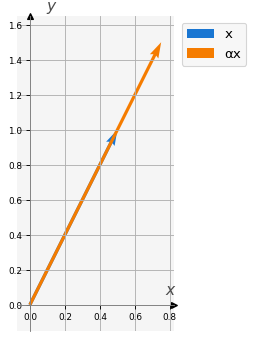
\includegraphics{05_Conduccion_NO_estacionaria_files/figure-pdf/cell-10-output-2.png}

\section{Ejercicio 2.}\label{ejercicio-2.-2}

Realiza los siguiente gráficos de la solución anterior: 1. Contornos
llenos (\texttt{contourf}) y líneas de contorno negras sobrepuestas
(\texttt{contour}). 2. Almacena el error en cada iteración y grafícalo
en semi-log. 3. Realiza las dos gráficas anteriores en un solo renglón.

\begin{Shaded}
\begin{Highlighting}[]
\NormalTok{plt.contour(xg, yg, u, cmap}\OperatorTok{=}\StringTok{\textquotesingle{}gray\textquotesingle{}}\NormalTok{, levels}\OperatorTok{=}\DecValTok{5}\NormalTok{)}
\NormalTok{plt.contourf(xg, yg, u, levels}\OperatorTok{=}\DecValTok{50}\NormalTok{, cmap}\OperatorTok{=}\StringTok{\textquotesingle{}inferno\textquotesingle{}}\NormalTok{)}
\end{Highlighting}
\end{Shaded}

\includegraphics{05_Conduccion_NO_estacionaria_files/figure-pdf/cell-11-output-1.png}

\begin{Shaded}
\begin{Highlighting}[]
\NormalTok{plt.plot(error\_lista)}
\NormalTok{plt.yscale(}\StringTok{\textquotesingle{}log\textquotesingle{}}\NormalTok{)}
\end{Highlighting}
\end{Shaded}

\includegraphics{05_Conduccion_NO_estacionaria_files/figure-pdf/cell-12-output-1.png}

\begin{Shaded}
\begin{Highlighting}[]
\NormalTok{fig }\OperatorTok{=}\NormalTok{ plt.figure()}

\NormalTok{ax1 }\OperatorTok{=}\NormalTok{ fig.add\_subplot(}\DecValTok{1}\NormalTok{, }\DecValTok{2}\NormalTok{, }\DecValTok{1}\NormalTok{)}
\NormalTok{ax2 }\OperatorTok{=}\NormalTok{ fig.add\_subplot(}\DecValTok{1}\NormalTok{, }\DecValTok{2}\NormalTok{, }\DecValTok{2}\NormalTok{)}

\NormalTok{ax1.contour(xg, yg, u, cmap}\OperatorTok{=}\StringTok{\textquotesingle{}gray\textquotesingle{}}\NormalTok{, levels}\OperatorTok{=}\DecValTok{5}\NormalTok{)}
\NormalTok{ax1.contourf(xg, yg, u, levels}\OperatorTok{=}\DecValTok{50}\NormalTok{, cmap}\OperatorTok{=}\StringTok{\textquotesingle{}inferno\textquotesingle{}}\NormalTok{)}

\NormalTok{ax2.plot(error\_lista)}
\NormalTok{ax2.set\_yscale(}\StringTok{\textquotesingle{}log\textquotesingle{}}\NormalTok{)}

\NormalTok{plt.tight\_layout()}
\end{Highlighting}
\end{Shaded}

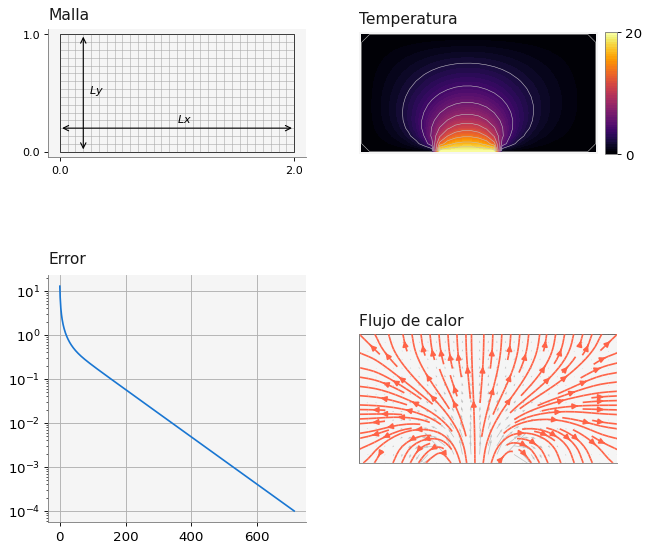
\includegraphics{05_Conduccion_NO_estacionaria_files/figure-pdf/cell-13-output-1.png}

\section{Flujo de calor}\label{flujo-de-calor-1}

Fourier también estableció una ley para el flujo de calor que se escribe
como:

\[
\vec{q} = -\kappa \nabla u = -\kappa \left(\dfrac{\partial u}{\partial x}, \dfrac{\partial u}{\partial y}\right)
\]

\section{Ejercicio 3.}\label{ejercicio-3.-2}

Usando la información calculada de la temperatura (almacenada en el
arreglo \texttt{u}), vamos a calcular el flujo de calor usando la
siguiente fórmula en diferencias:

\[
\vec{q}_{i,j} = (qx_{i,j}, qy_{i,j}) = -\dfrac{\kappa}{2h} (u_{i+1,j}-u_{i-1,j}, u_{i,j+1}-u_{i,j-1} )
\]

\begin{Shaded}
\begin{Highlighting}[]
\NormalTok{qx }\OperatorTok{=}\NormalTok{ np.zeros((Nx}\OperatorTok{+}\DecValTok{2}\NormalTok{, Ny}\OperatorTok{+}\DecValTok{2}\NormalTok{))}
\NormalTok{qy }\OperatorTok{=}\NormalTok{ qx.copy()}

\NormalTok{s }\OperatorTok{=}\NormalTok{ k }\OperatorTok{/} \DecValTok{2}\OperatorTok{*}\NormalTok{h}
\ControlFlowTok{for}\NormalTok{ i }\KeywordTok{in} \BuiltInTok{range}\NormalTok{(}\DecValTok{1}\NormalTok{,Nx}\OperatorTok{+}\DecValTok{1}\NormalTok{):}
    \ControlFlowTok{for}\NormalTok{ j }\KeywordTok{in} \BuiltInTok{range}\NormalTok{(}\DecValTok{1}\NormalTok{,Ny}\OperatorTok{+}\DecValTok{1}\NormalTok{):}
\NormalTok{        qx[i,j] }\OperatorTok{=} \OperatorTok{{-}}\NormalTok{s }\OperatorTok{*}\NormalTok{ (u[i}\OperatorTok{+}\DecValTok{1}\NormalTok{,j] }\OperatorTok{{-}}\NormalTok{ u[i}\OperatorTok{{-}}\DecValTok{1}\NormalTok{,j])}
\NormalTok{        qy[i,j] }\OperatorTok{=} \OperatorTok{{-}}\NormalTok{s }\OperatorTok{*}\NormalTok{ (u[i,j}\OperatorTok{+}\DecValTok{1}\NormalTok{] }\OperatorTok{{-}}\NormalTok{ u[i,j}\OperatorTok{{-}}\DecValTok{1}\NormalTok{])}

\NormalTok{plt.quiver(xg, yg, qx, qy, scale}\OperatorTok{=}\DecValTok{10}\NormalTok{, zorder}\OperatorTok{=}\DecValTok{10}\NormalTok{)}
\end{Highlighting}
\end{Shaded}

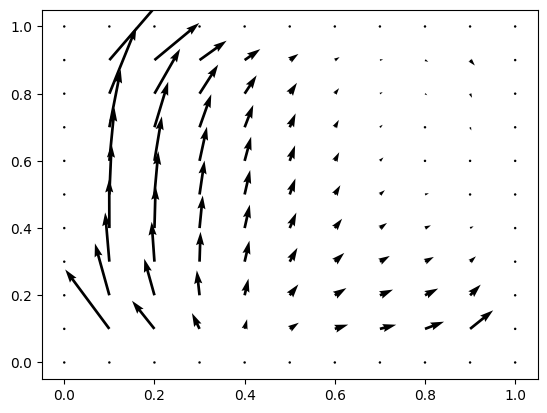
\includegraphics{05_Conduccion_NO_estacionaria_files/figure-pdf/cell-14-output-1.png}

\section{Ejercicio 4.}\label{ejercicio-4.-1}

Grafica el campo vectorial del flujo de calor, junto con los contornos
de la temperatura (\texttt{contourf} y \texttt{contour}). Haz que tu
gráfica se vea con razón de aspecto correcta de 1 por 1.

\begin{Shaded}
\begin{Highlighting}[]
\NormalTok{plt.contour(xg, yg, u, cmap}\OperatorTok{=}\StringTok{\textquotesingle{}gray\textquotesingle{}}\NormalTok{, levels}\OperatorTok{=}\DecValTok{5}\NormalTok{)}
\NormalTok{plt.contourf(xg, yg, u, levels}\OperatorTok{=}\DecValTok{50}\NormalTok{, cmap}\OperatorTok{=}\StringTok{\textquotesingle{}cool\textquotesingle{}}\NormalTok{, zorder}\OperatorTok{=}\DecValTok{1}\NormalTok{)}
\NormalTok{plt.quiver(xg, yg, qx, qy, scale}\OperatorTok{=}\DecValTok{10}\NormalTok{, zorder}\OperatorTok{=}\DecValTok{10}\NormalTok{)}
\NormalTok{ax }\OperatorTok{=}\NormalTok{ plt.gca()}
\NormalTok{ax.set\_aspect(}\StringTok{\textquotesingle{}equal\textquotesingle{}}\NormalTok{)}
\end{Highlighting}
\end{Shaded}

\includegraphics{05_Conduccion_NO_estacionaria_files/figure-pdf/cell-15-output-1.png}

\bookmarksetup{startatroot}

\chapter{Seguimiento de partículas}\label{seguimiento-de-partuxedculas}

Si soltamos una partícula en un flujo, dicha partícula seguirá la
dirección del flujo y delineará una trayectoria como se muestra en la
siguiente figura. Para calcular los puntos de la trayectoria debemos
resolver una ecuación como la siguiente:

\[
\dfrac{\partial \vec{x}}{ \partial t} = \vec{v} \qquad \text{con} \qquad \vec{x}(t=0) = \vec{x}_o 
\]

donde \$\vec{x} = (x,y) \$ representa la posición de la partícula y
\(\vec{v} = (vx, vy)\) su velocidad. El método más sencillo para
encontrar las posiciones de la partícula es conocido como de \emph{Euler
hacia adelante} y se escribe como:

\[
\vec{x}_i^{n+1} = \vec{x}_i^{n} + h_t * \vec{v}_{i}^n
\]

donde \(\vec{x}_i^{n}\) representa la posición de la partícula \(i\) en
el instante \(n\), \(h_t\) es el paso de tiempo y \(\vec{v}_i\) es la
velocidad en la partícula \(i\) en el instante \(n\).

\section{Ejercicio 5.}\label{ejercicio-5.}

Calcular y graficar las trayectorias de varias partículas usando el
campo vectorial generado por el flujo de calor del ejemplo 2.

Escribimos la fórmula de \emph{Euler hacia adelante} en componentes como
sigue:

\[
\begin{eqnarray}
x_i^{n+1} & = & x_i^{n} + h_t * vx_{i}^n \\
y_i^{n+1} & = & y_i^{n} + h_t * vy_{i}^n 
\end{eqnarray}
\]

\textbf{1. Definimos un punto inicial de forma aleatoria en el cuadrado
unitario:}

\begin{Shaded}
\begin{Highlighting}[]
\NormalTok{xo }\OperatorTok{=} \FloatTok{0.2} \CommentTok{\#np.random.rand(1)}
\NormalTok{yo }\OperatorTok{=} \FloatTok{0.5} \CommentTok{\#np.random.rand(1)}
\BuiltInTok{print}\NormalTok{(xo)}
\BuiltInTok{print}\NormalTok{(yo)}
\end{Highlighting}
\end{Shaded}

\begin{verbatim}
0.2
0.5
\end{verbatim}

\textbf{2. Definimos arreglos para almacenar las coordenadas de la
trayectoria:}

\begin{Shaded}
\begin{Highlighting}[]
\NormalTok{Pasos }\OperatorTok{=} \DecValTok{10}
\NormalTok{xp }\OperatorTok{=}\NormalTok{ np.zeros(Pasos)}
\NormalTok{yp }\OperatorTok{=}\NormalTok{ np.zeros(Pasos)}
\NormalTok{xp[}\DecValTok{0}\NormalTok{] }\OperatorTok{=}\NormalTok{ xo}
\NormalTok{yp[}\DecValTok{0}\NormalTok{] }\OperatorTok{=}\NormalTok{ yo}
\BuiltInTok{print}\NormalTok{(xp)}
\BuiltInTok{print}\NormalTok{(yp)}
\end{Highlighting}
\end{Shaded}

\begin{verbatim}
[0.2 0.  0.  0.  0.  0.  0.  0.  0.  0. ]
[0.5 0.  0.  0.  0.  0.  0.  0.  0.  0. ]
\end{verbatim}

\begin{Shaded}
\begin{Highlighting}[]
\NormalTok{plt.plot(xp[}\DecValTok{0}\NormalTok{], yp[}\DecValTok{0}\NormalTok{], }\StringTok{\textquotesingle{}o{-}\textquotesingle{}}\NormalTok{)}
\NormalTok{plt.xlim(}\DecValTok{0}\NormalTok{,}\DecValTok{1}\NormalTok{)}
\NormalTok{plt.ylim(}\DecValTok{0}\NormalTok{,}\DecValTok{1}\NormalTok{)}
\end{Highlighting}
\end{Shaded}

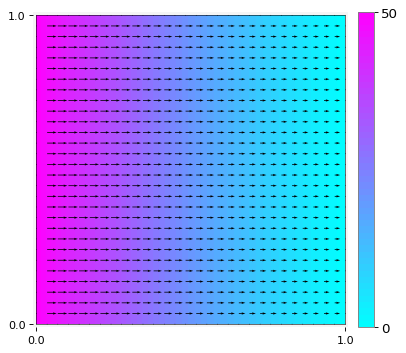
\includegraphics{05_Conduccion_NO_estacionaria_files/figure-pdf/cell-18-output-1.png}

\textbf{3. Implementamos el método de Euler hacia adelante}:

\begin{Shaded}
\begin{Highlighting}[]
\CommentTok{\# Interpolación de la velocidad}
\KeywordTok{def}\NormalTok{ interpolaVel(qx, qy, xpi, ypi, h):}
    \CommentTok{\# localizamos la partícula dentro de la rejilla:}
\NormalTok{    li }\OperatorTok{=} \BuiltInTok{int}\NormalTok{(xpi}\OperatorTok{/}\NormalTok{h)}
\NormalTok{    lj }\OperatorTok{=} \BuiltInTok{int}\NormalTok{(ypi}\OperatorTok{/}\NormalTok{h)}
    \ControlFlowTok{return}\NormalTok{ (qx[li,lj], qy[li,lj])}
\end{Highlighting}
\end{Shaded}

\begin{Shaded}
\begin{Highlighting}[]
\NormalTok{ht }\OperatorTok{=} \FloatTok{0.1}
\ControlFlowTok{for}\NormalTok{ n }\KeywordTok{in} \BuiltInTok{range}\NormalTok{(}\DecValTok{1}\NormalTok{,Pasos):}
\NormalTok{    vx, vy }\OperatorTok{=}\NormalTok{ interpolaVel(qx, qy, xp[n}\OperatorTok{{-}}\DecValTok{1}\NormalTok{], yp[n}\OperatorTok{{-}}\DecValTok{1}\NormalTok{], h)}
\NormalTok{    xp[n] }\OperatorTok{=}\NormalTok{ xp[n}\OperatorTok{{-}}\DecValTok{1}\NormalTok{] }\OperatorTok{+}\NormalTok{ ht }\OperatorTok{*}\NormalTok{ vx}
\NormalTok{    yp[n] }\OperatorTok{=}\NormalTok{ yp[n}\OperatorTok{{-}}\DecValTok{1}\NormalTok{] }\OperatorTok{+}\NormalTok{ ht }\OperatorTok{*}\NormalTok{ vy}
\end{Highlighting}
\end{Shaded}

\begin{Shaded}
\begin{Highlighting}[]
\BuiltInTok{print}\NormalTok{(xp)}
\BuiltInTok{print}\NormalTok{(yp)}
\end{Highlighting}
\end{Shaded}

\begin{verbatim}
[0.2        0.21738397 0.23476794 0.25215191 0.26953588 0.28691984
 0.31035226 0.32940321 0.34845415 0.36750509]
[0.5        0.52197449 0.54394898 0.56592346 0.58789795 0.60987244
 0.62441928 0.64213907 0.65985885 0.67757864]
\end{verbatim}

\begin{Shaded}
\begin{Highlighting}[]
\NormalTok{plt.plot(xp, yp, }\StringTok{\textquotesingle{}.{-}\textquotesingle{}}\NormalTok{)}
\NormalTok{plt.xlim(}\DecValTok{0}\NormalTok{,}\DecValTok{1}\NormalTok{)}
\NormalTok{plt.ylim(}\DecValTok{0}\NormalTok{,}\DecValTok{1}\NormalTok{)}
\end{Highlighting}
\end{Shaded}

\includegraphics{05_Conduccion_NO_estacionaria_files/figure-pdf/cell-22-output-1.png}

\section{Ejercicio 6.}\label{ejercicio-6.}

Dibuja la trayectoria de la siguiente manera. - El primer punto color
naranja transparente y contorno negro. - Las posiciones siguientes de
color negro sobre puestas sobre la trayectoria. - La trayectoria de
color gris. - Verifica que la trayectoria no se salga del cuadrado
unitario.

\begin{Shaded}
\begin{Highlighting}[]
\NormalTok{plt.figure(figsize}\OperatorTok{=}\NormalTok{(}\DecValTok{5}\NormalTok{,}\DecValTok{5}\NormalTok{))}
\NormalTok{plt.scatter(xp[}\DecValTok{0}\NormalTok{], yp[}\DecValTok{0}\NormalTok{], c}\OperatorTok{=}\StringTok{\textquotesingle{}orange\textquotesingle{}}\NormalTok{, edgecolor}\OperatorTok{=}\StringTok{\textquotesingle{}k\textquotesingle{}}\NormalTok{, alpha}\OperatorTok{=}\FloatTok{0.5}\NormalTok{)}
\NormalTok{plt.plot(xp, yp, c}\OperatorTok{=}\StringTok{\textquotesingle{}gray\textquotesingle{}}\NormalTok{)}
\NormalTok{plt.scatter(xp[}\DecValTok{1}\NormalTok{:], yp[}\DecValTok{1}\NormalTok{:], c}\OperatorTok{=}\StringTok{\textquotesingle{}k\textquotesingle{}}\NormalTok{, s}\OperatorTok{=}\DecValTok{10}\NormalTok{, zorder}\OperatorTok{=}\DecValTok{5}\NormalTok{)}
\NormalTok{plt.xlim(}\DecValTok{0}\NormalTok{,}\DecValTok{1}\NormalTok{)}
\NormalTok{plt.ylim(}\DecValTok{0}\NormalTok{,}\DecValTok{1}\NormalTok{)}
\NormalTok{ax }\OperatorTok{=}\NormalTok{ plt.gca()}
\NormalTok{ax.set\_aspect(}\StringTok{\textquotesingle{}equal\textquotesingle{}}\NormalTok{)}
\NormalTok{plt.savefig(}\StringTok{\textquotesingle{}trayectoria1.pdf\textquotesingle{}}\NormalTok{)}
\end{Highlighting}
\end{Shaded}

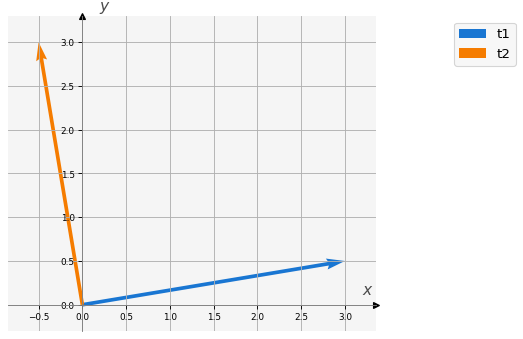
\includegraphics{05_Conduccion_NO_estacionaria_files/figure-pdf/cell-23-output-1.png}

\section{Ejercicio 7.}\label{ejercicio-7.}

Dibuja varias trayectorias que inicien en sitios diferentes.

\section{Ejercicio 8.}\label{ejercicio-8.}

Implementa una interpolación bilineal para calcular la velocidad.

\bookmarksetup{startatroot}

\chapter{Conducción de calor en 2D: algoritmos de solución de sistemas
de
ecuaciones.}\label{conducciuxf3n-de-calor-en-2d-algoritmos-de-soluciuxf3n-de-sistemas-de-ecuaciones.}

\textbf{Objetivo}.

Comparar mediante un interactivo varios métodos de solución de sistemas
de ecuaciones lineales.

MACTI-Analisis\_Numerico\_01 by Luis M. de la Cruz is licensed under
Attribution-ShareAlike 4.0 International

\textbf{Trabajo realizado con el apoyo del Programa UNAM-DGAPA-PAPIME
PE101922}

Al ejecutar la siguiente celda obtendrás un interactivo en donde podrás
seleccionar el método de solución y el tamaño de la malla
(\(M \times N\)) para resolver numéricamente, por diferencias finitas,
un problema de conducción de calor.

Analiza con cuidado los valores más óptimos para encontrar una buena
solución.

\textbf{NOTA}. Para ejecutar el interactivo debes hacer clic en el botón
de play (a la derecha).

\begin{Shaded}
\begin{Highlighting}[]
\OperatorTok{\%}\NormalTok{run }\StringTok{"./zHeatCondSolvers.py"}
\end{Highlighting}
\end{Shaded}

\begin{verbatim}
VBox(children=(HBox(children=(Dropdown(description='Método', layout=Layout(height='auto', width='auto'), optio…
\end{verbatim}

\begin{verbatim}
Output()
\end{verbatim}

\bookmarksetup{startatroot}

\chapter{Flujo Monofásico en 2D con Algoritmo de
Thomas}\label{flujo-monofuxe1sico-en-2d-con-algoritmo-de-thomas}

\textbf{Objetivo general} - El alumno resolverá la ecuación de Laplace
en dos dimensiones, la cual representa el flujo monofásico incompresible
en estado estable, con propiedades del fluido y del medio constantes.
Mediante la solución de esta ecuación, se conocerán los tipos de
condiciones de frontera y los tipos de solvers que se aplican en la
solución de problemas relacionados con la Simulación Matemática de
Yacimientos (SMY).

\textbf{Objetivos particulares} - Conocer e identificar los tipos de
condiciones a la frontera utilizadas en SMY. - Identificar la dirección
del flujo de fluidos de acuerdo a las isobaras.

\textbf{Trabajo realizado con el apoyo del Programa UNAM-DGAPA-PAPIME
PE101922}

\section{Contenido}\label{contenido}

\begin{itemize}
\tightlist
\item
  \hyperref[1]{1 - Resolución de un problema de ingeniería mediante
  matemática computacional}
\item
  \hyperref[2]{2 - Condiciones de frontera}

  \begin{itemize}
  \tightlist
  \item
    \hyperref[2.1]{2.1 - Primera clase (Neumann)}
  \item
    \hyperref[2.2]{2.2 - Segunda clase (Dirichlet)}
  \item
    \hyperref[ej-1]{Ejercicio 1.}
  \end{itemize}
\item
  \hyperref[3]{3 - Resolución del problema para flujo monofasico en 2D}

  \begin{itemize}
  \tightlist
  \item
    \hyperref[3.1]{3.1 - Algoritmo de Thomas.}
  \item
    \hyperref[ej-2]{Ejercicio 2}
  \end{itemize}
\end{itemize}

\#\# 1. Resolución de un problema de ingeniería mediante matemática
computacional Se realiza la siguiente metodología: 1. Definir un modelo
físico conceptual 2. Definir el modelo matemático 3. Definir el modelo
numérico 4. Definir el modelo computacional (algoritmo de solución)

\subsection{1.1 Modelo físico
conceptual}\label{modelo-fuxedsico-conceptual}

Se inyecta un fluido a presión constante (\textbf{1,000 psi}) y se
produce a presión constante (\textbf{500 psi}), en un medio poroso
bidimensional homogéneo (de longitud Lx = \textbf{1,000 ft} y Ly =
\textbf{500 ft} con permeabilidad y porosidad constantes), así mismo las
propiedades del fluido no dependen de la presión, adicionalmente el
medio poroso se encuentra saturado completamente de este fluido, por lo
que se desea conocer el gradiente de presión en estado permanente.

\begin{enumerate}
\def\labelenumi{\arabic{enumi}.}
\tightlist
\item
  No se consideran los efectos de la fuerza de gravedad
\item
  No hay fuentes ni sumideros
\item
  El fluido es incompresible y la viscosidad constante
\item
  El medio está inicialmente saturado del fluido
\item
  Ya se ha llegado al estado estable o permanente
\item
  Las permeabilidades en dirección \(x\) y \(y\) son iguales e
  invariantes en el espacio y tiempo
\end{enumerate}

Partiendo de la ecuacion general de balance de materia para flujo
monofásico (de cualquier fluido \(\alpha\)) en medios porosos se tiene:

\[\frac{\partial \phi\rho_\alpha}{\partial t} - \nabla (\rho_\alpha \frac{k}{\mu}(\nabla\rho_\alpha - \rho_\alpha \delta\nabla z)) = q_\alpha\]

\subsection{1.2 y 1.3 Modelo matemático y
numérico}\label{y-1.3-modelo-matemuxe1tico-y-numuxe9rico}

Tomando en cuenta las consideraciones del modelo físico se llega a:
\[\frac{\partial^2 \rho_\alpha}{\partial x^2} + \frac{\partial^2 \rho_\alpha}{\partial y^2} = 0\]

Discretizando la ecuacion anterior en una malla bidimensional se llega
a:

\[AP_{i,j}p_i = AE_{i,j}p_{i+1, j}+ AW_{i,j}p_{i-1, j} + AN_{i,j}p_{i,j+1} + AS_{i,j}p_{i-1, j} + B_{i,j}\]

\[i = 1,2,3,4,...,nx-2\] \[j = 1,2,3,4,...,ny-2\]

\begin{Shaded}
\begin{Highlighting}[]
\ImportTok{import}\NormalTok{ numpy }\ImportTok{as}\NormalTok{ np}
\ImportTok{import}\NormalTok{ matplotlib.pyplot }\ImportTok{as}\NormalTok{ plt}
\ImportTok{import}\NormalTok{ pandas }\ImportTok{as}\NormalTok{ pd}
\ImportTok{import}\NormalTok{ ipywidgets }\ImportTok{as}\NormalTok{ widgets}
\ImportTok{import}\NormalTok{ funciones\_personalizadas }\ImportTok{as}\NormalTok{ fp}

\ImportTok{from}\NormalTok{ matplotlib }\ImportTok{import}\NormalTok{ animation, cm}
\ImportTok{from}\NormalTok{ IPython.display }\ImportTok{import}\NormalTok{ HTML}
\end{Highlighting}
\end{Shaded}

\begin{Shaded}
\begin{Highlighting}[]
\CommentTok{\# Considere una malla rectangular de 1,000 ft x 500 ft, en el eje x e y, respectivamente. Con 5 nodos en x y 4 en y.}

\NormalTok{nodos\_x, nodos\_y }\OperatorTok{=} \DecValTok{5}\NormalTok{, }\DecValTok{4}
\NormalTok{longitud\_x, longitud\_y }\OperatorTok{=} \DecValTok{1000}\NormalTok{, }\DecValTok{500}
\NormalTok{nx\_a\_discretizar, ny\_a\_discretizar }\OperatorTok{=} \DecValTok{1}\NormalTok{,}\DecValTok{1}

\NormalTok{fp.discretizacion\_en\_malla\_rectangular(longitud\_x, longitud\_y, nodos\_y, nodos\_x, nx\_a\_discretizar, ny\_a\_discretizar)}
\end{Highlighting}
\end{Shaded}

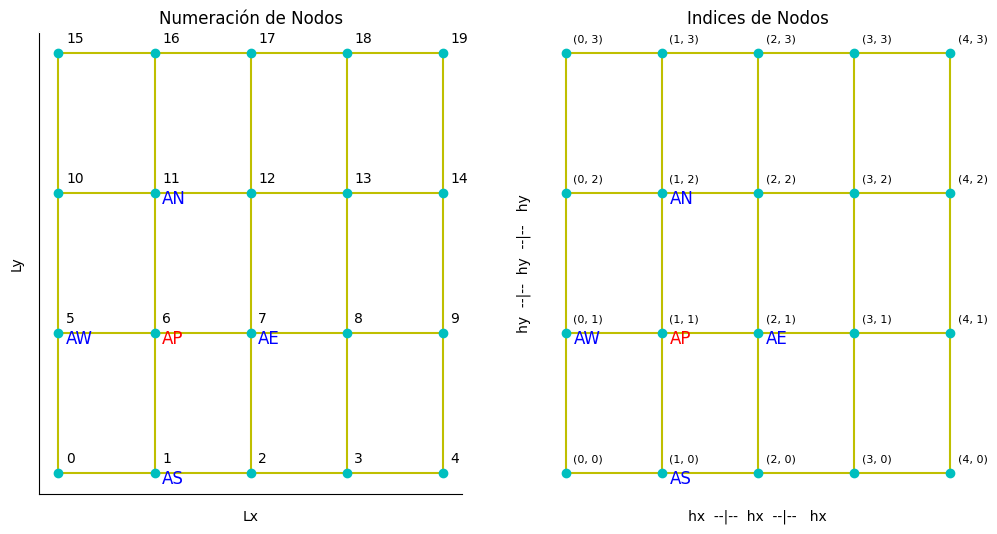
\includegraphics{07_Laplace_2D_Thomas_files/figure-pdf/cell-3-output-1.png}

\begin{verbatim}
Nodo discretizado: 
\end{verbatim}

\begin{Shaded}
\begin{Highlighting}[]
\NormalTok{nodos\_x, nodos\_y }\OperatorTok{=} \DecValTok{5}\NormalTok{, }\DecValTok{4}
\NormalTok{nodo\_a\_discretizar }\OperatorTok{=} \DecValTok{1}

\NormalTok{fp.generar\_matriz(nodos\_x, nodos\_y, nodo\_a\_discretizar)}
\end{Highlighting}
\end{Shaded}

\begin{longtable}[]{@{}lllllllllllllllllllll@{}}
\caption{}\label{T_0e862}\tabularnewline
\toprule\noalign{}
~ & 0 & 1 & 2 & 3 & 4 & 5 & 6 & 7 & 8 & 9 & 10 & 11 & 12 & 13 & 14 & 15
& 16 & 17 & 18 & 19 \\
\midrule\noalign{}
\endfirsthead
\toprule\noalign{}
~ & 0 & 1 & 2 & 3 & 4 & 5 & 6 & 7 & 8 & 9 & 10 & 11 & 12 & 13 & 14 & 15
& 16 & 17 & 18 & 19 \\
\midrule\noalign{}
\endhead
\bottomrule\noalign{}
\endlastfoot
0 & AP & AE & 0 & 0 & 0 & AN & 0 & 0 & 0 & 0 & 0 & 0 & 0 & 0 & 0 & 0 & 0
& 0 & 0 & 0 \\
1 & AW & AP & AE & 0 & 0 & 0 & AN & 0 & 0 & 0 & 0 & 0 & 0 & 0 & 0 & 0 &
0 & 0 & 0 & 0 \\
2 & 0 & AW & AP & AE & 0 & 0 & 0 & AN & 0 & 0 & 0 & 0 & 0 & 0 & 0 & 0 &
0 & 0 & 0 & 0 \\
3 & 0 & 0 & AW & AP & AE & 0 & 0 & 0 & AN & 0 & 0 & 0 & 0 & 0 & 0 & 0 &
0 & 0 & 0 & 0 \\
4 & 0 & 0 & 0 & AW & AP & 0 & 0 & 0 & 0 & AN & 0 & 0 & 0 & 0 & 0 & 0 & 0
& 0 & 0 & 0 \\
5 & AS & 0 & 0 & 0 & 0 & AP & AE & 0 & 0 & 0 & AN & 0 & 0 & 0 & 0 & 0 &
0 & 0 & 0 & 0 \\
6 & 0 & AS & 0 & 0 & 0 & AW & AP & AE & 0 & 0 & 0 & AN & 0 & 0 & 0 & 0 &
0 & 0 & 0 & 0 \\
7 & 0 & 0 & AS & 0 & 0 & 0 & AW & AP & AE & 0 & 0 & 0 & AN & 0 & 0 & 0 &
0 & 0 & 0 & 0 \\
8 & 0 & 0 & 0 & AS & 0 & 0 & 0 & AW & AP & AE & 0 & 0 & 0 & AN & 0 & 0 &
0 & 0 & 0 & 0 \\
9 & 0 & 0 & 0 & 0 & AS & 0 & 0 & 0 & AW & AP & 0 & 0 & 0 & 0 & AN & 0 &
0 & 0 & 0 & 0 \\
10 & 0 & 0 & 0 & 0 & 0 & AS & 0 & 0 & 0 & 0 & AP & AE & 0 & 0 & 0 & AN &
0 & 0 & 0 & 0 \\
11 & 0 & 0 & 0 & 0 & 0 & 0 & AS & 0 & 0 & 0 & AW & AP & AE & 0 & 0 & 0 &
AN & 0 & 0 & 0 \\
12 & 0 & 0 & 0 & 0 & 0 & 0 & 0 & AS & 0 & 0 & 0 & AW & AP & AE & 0 & 0 &
0 & AN & 0 & 0 \\
13 & 0 & 0 & 0 & 0 & 0 & 0 & 0 & 0 & AS & 0 & 0 & 0 & AW & AP & AE & 0 &
0 & 0 & AN & 0 \\
14 & 0 & 0 & 0 & 0 & 0 & 0 & 0 & 0 & 0 & AS & 0 & 0 & 0 & AW & AP & 0 &
0 & 0 & 0 & AN \\
15 & 0 & 0 & 0 & 0 & 0 & 0 & 0 & 0 & 0 & 0 & AS & 0 & 0 & 0 & 0 & AP &
AE & 0 & 0 & 0 \\
16 & 0 & 0 & 0 & 0 & 0 & 0 & 0 & 0 & 0 & 0 & 0 & AS & 0 & 0 & 0 & AW &
AP & AE & 0 & 0 \\
17 & 0 & 0 & 0 & 0 & 0 & 0 & 0 & 0 & 0 & 0 & 0 & 0 & AS & 0 & 0 & 0 & AW
& AP & AE & 0 \\
18 & 0 & 0 & 0 & 0 & 0 & 0 & 0 & 0 & 0 & 0 & 0 & 0 & 0 & AS & 0 & 0 & 0
& AW & AP & AE \\
19 & 0 & 0 & 0 & 0 & 0 & 0 & 0 & 0 & 0 & 0 & 0 & 0 & 0 & 0 & AS & 0 & 0
& 0 & AW & AP \\
\end{longtable}

\subsection{Discretización de las
ecuaciones}\label{discretizaciuxf3n-de-las-ecuaciones}

Aplicando diferencias finitas centradas

\[\frac{\partial^2 \rho_\alpha}{\partial x^2}+ \frac{\partial^2\rho_\alpha}{\partial y^2} =
\frac{P_{i+1,j-1} - 2P_{i,j} + P_{i-1,j}}{hx^2}
+ \frac{P_{i,j+1} - 2P_{i,j} + P_{i,j-1}}{hy^2} = 0\]

Despejando \(P_{i,j}\) (donde P es el valor incognita)

\[P_{i,j}(\frac{2}{hx^2} + \frac{2}{hy^2})  
= \frac{P_{i+1,j}}{hx^2} + \frac{P_{i-1,j}}{hx^2} + \frac{P_{i,j+1}}{hy^2} + \frac{P_{i,j-1}}{hy^2}
\]

La ecuación anterior se puede reescribir como:
\[AP P_{i,j} = AE P_{i+1,j} + AW P_{i-1,j} + AN P_{i,j+1}
+ AS P_{i,j-1} + B_{i,j}\]

\(Donde:\)

\(AP = (\frac{2}{hx^2} + \frac{2}{hy^2})\), \(AE = \frac{1}{hx^2}\),
\(AW = \frac{1}{hx^2}\), \(AN = \frac{1}{hy^2}\),
\(AS = \frac{1}{hy^2}\),

\begin{Shaded}
\begin{Highlighting}[]
\KeywordTok{def}\NormalTok{ ecuaciones\_discretizadas(lx, ly, nx, ny, hx, hy):}
    \CommentTok{"""}
\CommentTok{    Esta funcion genera los coeficientes de la ecuacion de flujo monofasico discretizada. No se consideran las}
\CommentTok{    condiciones de frontera.}
\CommentTok{    Parametros}
\CommentTok{    {-}{-}{-}{-}{-}{-}{-}{-}{-}{-}}
\CommentTok{    lx, ly : entero o flotante.}
\CommentTok{        Longitud en el eje x e y.}
\CommentTok{    nx, ny : int, int.}
\CommentTok{        Nodos en de la malla rectangular.}
\CommentTok{    Retorna}
\CommentTok{    {-}{-}{-}{-}{-}{-}{-}}
\CommentTok{    AP,AE,AW,AN,AS,B : ndarray. }
\CommentTok{        Arreglos en 2D para generar una matriz pentadiagonal.}
\CommentTok{    """}
    
    \CommentTok{\# se definen los arreglos en dos dimensiones}
\NormalTok{    AP }\OperatorTok{=}\NormalTok{ np.zeros((nx,ny)) }
\NormalTok{    AE }\OperatorTok{=}\NormalTok{ np.zeros((nx,ny))}
\NormalTok{    AW }\OperatorTok{=}\NormalTok{ np.zeros((nx,ny))}
\NormalTok{    AN }\OperatorTok{=}\NormalTok{ np.zeros((nx,ny))}
\NormalTok{    AS }\OperatorTok{=}\NormalTok{ np.zeros((nx,ny))}
\NormalTok{    B }\OperatorTok{=}\NormalTok{ np.zeros((nx,ny))}
    
    \ControlFlowTok{for}\NormalTok{ j }\KeywordTok{in} \BuiltInTok{range}\NormalTok{ (}\DecValTok{1}\NormalTok{,ny}\OperatorTok{{-}}\DecValTok{1}\NormalTok{):}
        \ControlFlowTok{for}\NormalTok{ i }\KeywordTok{in} \BuiltInTok{range}\NormalTok{ (}\DecValTok{1}\NormalTok{,nx}\OperatorTok{{-}}\DecValTok{1}\NormalTok{):}
\NormalTok{            AP[i][j]}\OperatorTok{=}\FloatTok{2.0}\OperatorTok{/}\NormalTok{hx}\OperatorTok{**}\FloatTok{2.0}\OperatorTok{+}\FloatTok{2.0}\OperatorTok{/}\NormalTok{hy}\OperatorTok{**}\FloatTok{2.0}
\NormalTok{            AE[i][j]}\OperatorTok{=}\FloatTok{1.0}\OperatorTok{/}\NormalTok{hx}\OperatorTok{**}\FloatTok{2.0}
\NormalTok{            AW[i][j]}\OperatorTok{=}\FloatTok{1.0}\OperatorTok{/}\NormalTok{hx}\OperatorTok{**}\FloatTok{2.0}
\NormalTok{            AN[i][j]}\OperatorTok{=}\FloatTok{1.0}\OperatorTok{/}\NormalTok{hy}\OperatorTok{**}\FloatTok{2.0}
\NormalTok{            AS[i][j]}\OperatorTok{=}\FloatTok{1.0}\OperatorTok{/}\NormalTok{hy}\OperatorTok{**}\FloatTok{2.0}
\NormalTok{            B[i][j]}\OperatorTok{=}\FloatTok{0.0}

    \ControlFlowTok{return}\NormalTok{ AP,AE,AW,AN,AS,B}
\end{Highlighting}
\end{Shaded}

\#\# 2. Codiciones de frontera De acuerdo con la SEG Wiki, las
condiciones de frontera se aplican en el término integral superficial de
la ecuación integral de un campo y consiste en valores prescritos de la
solución y de las derivadas de la solución en la frontera. Cuando los
valores de campo se especifican las condiciones se denominan
\textbf{condiciones de Dirichlet}. Cuando se especifican las derivadas
las condiciones se llaman \textbf{condiciones de Neumann}.

\#\#\# 2.1 Primera clase o Dirichlet Esta condición indica una funcion
conocida que varia en el tiempo o un escalar dado (invariante en el
tiempo) en las fronteras, es decir:

\[p_1=f(t,y) \quad o \quad p1=cte_1 = 1,000 psi\]
\[p_2=f(t,x) \quad o \quad p1=cte_2 = 500 psi\]
\[p_3=f(t,y) \quad o \quad p1=cte_3 = 500 psi\]
\[p_4=f(t,x) \quad o \quad p1=cte_4 = 500 psi\]

\textbf{Implementación:} 1. Identificar las fronteras y los puntos de la
ecuacion discreta donde se implementará la condición 2. Llevar a cabo
las sustituciones pertinenters en cada ecuación discreta, para este
caso:

\[AP_{i,j}P_i = AE P_{i+1,j} + AW P_{i-1,j} + AN P_{i,j+1}
+ AS P_{i,j-1} + B_{i,j}\]

Considerando una malla con \textbf{nx = 5x} y \textbf{ny = 4}, se tiene
la siguiente figura:

\subsubsection{Para la frontera SUR:}\label{para-la-frontera-sur}

Tomando en cuenta la figura anterior, se puede apreciar que no existe
relacion con la presión \(Sur (i,j-1)\), por lo tanto, la ecuación se
reduce a:

\[AP_{i,j}p_{i} = AE P_{i+1,j} + AW P_{i-1,j} + AN P_{i,j+1}
+ B_{i,j}\]

En este caso el valor de presión está definido, por lo que el sistema de
ecuaciones de reduce a:

\[AP_{i,j}P_i = B_i\]

\[para \quad i=0,1,2,3,4 \quad j=0\]
\[donde \quad AP_{i,j}=1 \quad y \quad B_{i,j}=Cte_2\]

\emph{Todos los demás coeficientes se asignan a cero}

Para el resto de las fronteras se utiliza la misma lógica

\begin{Shaded}
\begin{Highlighting}[]
\KeywordTok{def}\NormalTok{ condiciones\_de\_frontera\_dirichlet(P1, P2, P3, P4, AP, AW, AE, AN, AS, B, nx, ny):}
    \CommentTok{"""}
\CommentTok{    Esta función modifica los coeficientes y asigna las condiciones de frotera de primera clase. }
\CommentTok{    """}
    \ControlFlowTok{for}\NormalTok{ i }\KeywordTok{in} \BuiltInTok{range}\NormalTok{ (}\DecValTok{1}\NormalTok{,nx}\OperatorTok{{-}}\DecValTok{1}\NormalTok{):}
\NormalTok{        AP[i][}\DecValTok{0}\NormalTok{]}\OperatorTok{=}\FloatTok{1.0}
\NormalTok{        AW[i][}\DecValTok{0}\NormalTok{]}\OperatorTok{=}\FloatTok{0.0}    
\NormalTok{        AE[i][}\DecValTok{0}\NormalTok{]}\OperatorTok{=}\FloatTok{0.0}      \CommentTok{\#Frontera sur}
\NormalTok{        AN[i][}\DecValTok{0}\NormalTok{]}\OperatorTok{=}\FloatTok{0.0}
\NormalTok{        B[i][}\DecValTok{0}\NormalTok{]}\OperatorTok{=}\NormalTok{P2}
            
\NormalTok{        AP[i][ny}\OperatorTok{{-}}\DecValTok{1}\NormalTok{]}\OperatorTok{=}\FloatTok{1.0}
\NormalTok{        AW[i][ny}\OperatorTok{{-}}\DecValTok{1}\NormalTok{]}\OperatorTok{=}\FloatTok{0.0}    
\NormalTok{        AE[i][ny}\OperatorTok{{-}}\DecValTok{1}\NormalTok{]}\OperatorTok{=}\FloatTok{0.0}    \CommentTok{\#Frontera norte}
\NormalTok{        AS[i][ny}\OperatorTok{{-}}\DecValTok{1}\NormalTok{]}\OperatorTok{=}\FloatTok{0.0}
\NormalTok{        B[i][ny}\OperatorTok{{-}}\DecValTok{1}\NormalTok{]}\OperatorTok{=}\NormalTok{P4}

    \ControlFlowTok{for}\NormalTok{ j }\KeywordTok{in} \BuiltInTok{range}\NormalTok{ (}\DecValTok{0}\NormalTok{,ny):}
\NormalTok{        AP[}\DecValTok{0}\NormalTok{][j]}\OperatorTok{=}\FloatTok{1.0}
\NormalTok{        AE[}\DecValTok{0}\NormalTok{][j]}\OperatorTok{=}\FloatTok{0.0}      \CommentTok{\#Frontera Oeste}
\NormalTok{        AN[}\DecValTok{0}\NormalTok{][j]}\OperatorTok{=}\FloatTok{0.0}
\NormalTok{        AS[}\DecValTok{0}\NormalTok{][j]}\OperatorTok{=}\FloatTok{0.0}
\NormalTok{        B[}\DecValTok{0}\NormalTok{][j]}\OperatorTok{=}\NormalTok{P1}
        
\NormalTok{        AP[nx}\OperatorTok{{-}}\DecValTok{1}\NormalTok{][j]}\OperatorTok{=}\FloatTok{1.0}
\NormalTok{        AW[nx}\OperatorTok{{-}}\DecValTok{1}\NormalTok{][j]}\OperatorTok{=}\FloatTok{0.0}
\NormalTok{        AN[nx}\OperatorTok{{-}}\DecValTok{1}\NormalTok{][j]}\OperatorTok{=}\FloatTok{0.0}   \CommentTok{\#Frontera Este}
\NormalTok{        AS[nx}\OperatorTok{{-}}\DecValTok{1}\NormalTok{][j]}\OperatorTok{=}\FloatTok{0.0}
\NormalTok{        B[nx}\OperatorTok{{-}}\DecValTok{1}\NormalTok{][j]}\OperatorTok{=}\NormalTok{P3}
\end{Highlighting}
\end{Shaded}

\#\#\# 2.2 Fronteras de segunda clase Neumann (No flujo o frontera
cerrada) Éstas especifican la derivada normal a la frontera para ser
cero o constante.

\[p_1=f(t,y) \quad o \quad p1=cte_1 = 1,000 psi\]

\[ \frac{dp}{dy}\big|_{ 2} = f(t,x) \quad o \quad \frac{dp}{dy}\big|_{ 2} = 0.0\]

\[p_3=f(t,y) \quad o \quad p1=cte_3 = 500 psi\]

\[ \frac{dp}{dy}\big|_{ 4} = f(t,x) \quad o \quad \frac{dp}{dy}\big|_{ 4} = 0.0\]

Discretización:

\textbf{Frontera Sur:} \[\frac{dp}{dy}\big|_{ 2} = 0.0\]

Sustituyendo una diferencia adelantada:
\[\frac{P_{i,j+1}-P_{i,j}}{hy} = 0\]

\[P_{i,j+1} = P_{i,j}\]

\textbf{Frontera Norte:} \[\frac{dp}{dy}\big|_{ 2} = 0.0\]

Sustituyendo una diferencia atrasada:
\[\frac{P_{i,j}-P_{i,j-1}}{hy} = 0\]

\[P_{i,j} = P_{i,j-1}\]

\begin{Shaded}
\begin{Highlighting}[]
\KeywordTok{def}\NormalTok{ condiciones\_de\_frontera\_neumann(x, P1, P2, P3, P4, AP, AW, AE, AN, AS, B, nx, ny):}
    \CommentTok{"""}
\CommentTok{    Esta función modifica los coeficientes de la matriz y asigna las condiciones de frontera de segunda clase. }
\CommentTok{    """}
    
    \ControlFlowTok{for}\NormalTok{ i }\KeywordTok{in} \BuiltInTok{range}\NormalTok{ (}\DecValTok{1}\NormalTok{, nx}\OperatorTok{{-}}\DecValTok{1}\NormalTok{):}
\NormalTok{        AP[i][}\DecValTok{0}\NormalTok{]}\OperatorTok{=}\FloatTok{1.0}
\NormalTok{        AW[i][}\DecValTok{0}\NormalTok{]}\OperatorTok{=}\FloatTok{0.0}    
\NormalTok{        AE[i][}\DecValTok{0}\NormalTok{]}\OperatorTok{=}\FloatTok{0.0}      \CommentTok{\#Frontera sur}
\NormalTok{        AN[i][}\DecValTok{0}\NormalTok{]}\OperatorTok{=}\FloatTok{1.0}
\NormalTok{        B[i][}\DecValTok{0}\NormalTok{]}\OperatorTok{=}\DecValTok{0}
        
\NormalTok{        AP[i][ny}\OperatorTok{{-}}\DecValTok{1}\NormalTok{]}\OperatorTok{=}\FloatTok{1.0}
\NormalTok{        AW[i][ny}\OperatorTok{{-}}\DecValTok{1}\NormalTok{]}\OperatorTok{=}\FloatTok{0.0}    
\NormalTok{        AE[i][ny}\OperatorTok{{-}}\DecValTok{1}\NormalTok{]}\OperatorTok{=}\FloatTok{0.0}    \CommentTok{\#Frontera norte}
\NormalTok{        AS[i][ny}\OperatorTok{{-}}\DecValTok{1}\NormalTok{]}\OperatorTok{=}\FloatTok{1.0}
\NormalTok{        B[i][ny}\OperatorTok{{-}}\DecValTok{1}\NormalTok{]}\OperatorTok{=}\FloatTok{0.0}
    
    \ControlFlowTok{for}\NormalTok{ j }\KeywordTok{in} \BuiltInTok{range}\NormalTok{ (}\DecValTok{0}\NormalTok{,ny):}
\NormalTok{        AP[}\DecValTok{0}\NormalTok{][j]}\OperatorTok{=}\FloatTok{1.0}
\NormalTok{        AE[}\DecValTok{0}\NormalTok{][j]}\OperatorTok{=}\FloatTok{0.0}      \CommentTok{\#Frontera Oeste}
\NormalTok{        AN[}\DecValTok{0}\NormalTok{][j]}\OperatorTok{=}\FloatTok{0.0}
\NormalTok{        AS[}\DecValTok{0}\NormalTok{][j]}\OperatorTok{=}\FloatTok{0.0}
\NormalTok{        B[}\DecValTok{0}\NormalTok{][j]}\OperatorTok{=}\NormalTok{P1}
        
\NormalTok{        AP[nx}\OperatorTok{{-}}\DecValTok{1}\NormalTok{][j]}\OperatorTok{=}\FloatTok{1.0}
\NormalTok{        AW[nx}\OperatorTok{{-}}\DecValTok{1}\NormalTok{][j]}\OperatorTok{=}\FloatTok{0.0}
\NormalTok{        AN[nx}\OperatorTok{{-}}\DecValTok{1}\NormalTok{][j]}\OperatorTok{=}\FloatTok{0.0}   \CommentTok{\#Frontera Este}
\NormalTok{        AS[nx}\OperatorTok{{-}}\DecValTok{1}\NormalTok{][j]}\OperatorTok{=}\FloatTok{0.0}
\NormalTok{        B[nx}\OperatorTok{{-}}\DecValTok{1}\NormalTok{][j]}\OperatorTok{=}\NormalTok{P3}
\end{Highlighting}
\end{Shaded}

\#\# 3. Resolución del problema para flujo monofásico en 2D

Los pasos para resolver el problema de flujo monofásico en 2D se
presentan en el siguiente algoritmo: - Definir las variables del
problema (nodos, longitudes, etc) - Implementar las ecuaciones
discretizadas - Aplicar las condiciones de frontera - \textbf{Resolver
la matriz con algún solver}

A continuación se mostraran una comparativa entre el algortimo de Thomas
y las alternativas de SciPy.

\#\#\# 3.1 Solución mediante el Algortimo de Thomas

\begin{Shaded}
\begin{Highlighting}[]
\CommentTok{\# variables del problema}
\NormalTok{nx, ny }\OperatorTok{=} \DecValTok{10}\NormalTok{, }\DecValTok{10}
\NormalTok{lx, ly }\OperatorTok{=} \DecValTok{500}\NormalTok{, }\DecValTok{500}

\CommentTok{\#Generación de malla para graficar}
\NormalTok{x }\OperatorTok{=}\NormalTok{ np.linspace(}\DecValTok{0}\NormalTok{, lx, nx)}
\NormalTok{y }\OperatorTok{=}\NormalTok{ np.linspace(}\DecValTok{0}\NormalTok{, ly, ny)}
\NormalTok{malla\_x, malla\_y }\OperatorTok{=}\NormalTok{ np.meshgrid(x, y)}
\end{Highlighting}
\end{Shaded}

\begin{Shaded}
\begin{Highlighting}[]
\KeywordTok{def}\NormalTok{ flujo\_monofasico\_2d\_thomas(i):}
    \CommentTok{"""}
\CommentTok{    Esta funcion aplica el algoritmo de Thomas para resolver el problema de flujo monofasico en 2D.}
\CommentTok{    """}
    
    \CommentTok{"""}
\CommentTok{        |{-}{-}{-}P4(NORTE){-}{-}{-}|}
\CommentTok{        |               |}
\CommentTok{    P1(OESTE)        P3(ESTE)}
\CommentTok{        |               |}
\CommentTok{        |{-}{-}{-}{-}P2(SUR){-}{-}{-}{-}|}
\CommentTok{    }
\CommentTok{    donde P es presión (psi)}
\CommentTok{    """}
\NormalTok{    P1 }\OperatorTok{=} \DecValTok{700}\OperatorTok{+}\NormalTok{(i}\OperatorTok{*}\DecValTok{10}\NormalTok{)}
\NormalTok{    P2, P3, P4  }\OperatorTok{=} \FloatTok{500.0}\NormalTok{, }\FloatTok{500.0}\NormalTok{, }\FloatTok{500.0}
\NormalTok{    Press }\OperatorTok{=}\NormalTok{ np.zeros((nx,ny))}

    \CommentTok{\# se calcula el espaciamiento entre nodos}
\NormalTok{    hx }\OperatorTok{=}\NormalTok{ lx}\OperatorTok{/}\NormalTok{(nx}\OperatorTok{{-}}\DecValTok{1}\NormalTok{)}
\NormalTok{    hy }\OperatorTok{=}\NormalTok{ ly}\OperatorTok{/}\NormalTok{(ny}\OperatorTok{{-}}\DecValTok{1}\NormalTok{)}
    
    \CommentTok{\# Llamar a la función para obtener los coeficientes}
\NormalTok{    AP, AW, AE, AN, AS, B }\OperatorTok{=}\NormalTok{ ecuaciones\_discretizadas(lx, ly, nx, ny, hx, hy)}
    
    \CommentTok{"""}
\CommentTok{    Ejercicio 1 y Ejercicio 2}
\CommentTok{    }
\CommentTok{    Modificar {-}{-}{-}{-}{-}.}
\CommentTok{                   v}
\CommentTok{    """}
    \CommentTok{\#Aplicar condiciones de frontera}
\NormalTok{    condiciones\_de\_frontera\_dirichlet(P1, P2, P3, P4, AP, AW, AE, AN, AS, B, nx, ny)}
    
    \CommentTok{\# Resolver mediante Thomas}
\NormalTok{    iteramax, eps }\OperatorTok{=} \DecValTok{3000}\NormalTok{, }\FloatTok{1.0E{-}04}
\NormalTok{    fp.algoritmo\_thomas\_2D(nx, ny, AP, AE, AW, AN, AS, B, Press, iteramax, eps)}
    
\NormalTok{    u }\OperatorTok{=}\NormalTok{ np.zeros((nx,ny)) }
\NormalTok{    v }\OperatorTok{=}\NormalTok{ np.zeros((nx,ny)) }
    
    \ControlFlowTok{for}\NormalTok{ j }\KeywordTok{in} \BuiltInTok{range}\NormalTok{ (}\DecValTok{1}\NormalTok{,ny}\OperatorTok{{-}}\DecValTok{1}\NormalTok{):}
        \ControlFlowTok{for}\NormalTok{ i }\KeywordTok{in} \BuiltInTok{range}\NormalTok{ (}\DecValTok{1}\NormalTok{,nx}\OperatorTok{{-}}\DecValTok{1}\NormalTok{):}
\NormalTok{            u[i][j]}\OperatorTok{={-}}\NormalTok{(Press[i}\OperatorTok{+}\DecValTok{1}\NormalTok{][j]}\OperatorTok{{-}}\NormalTok{Press[i}\OperatorTok{{-}}\DecValTok{1}\NormalTok{][j])}\OperatorTok{/}\NormalTok{(}\DecValTok{2}\OperatorTok{*}\NormalTok{hx)  }\CommentTok{\#Discretizamos por DFC de primer orden}
\NormalTok{            v[i][j]}\OperatorTok{={-}}\NormalTok{(Press[i][j}\OperatorTok{+}\DecValTok{1}\NormalTok{]}\OperatorTok{{-}}\NormalTok{Press[i][j}\OperatorTok{{-}}\DecValTok{1}\NormalTok{])}\OperatorTok{/}\NormalTok{(}\DecValTok{2}\OperatorTok{*}\NormalTok{hy)}
    
    \ControlFlowTok{return}\NormalTok{ Press,u,v}
\end{Highlighting}
\end{Shaded}

\begin{Shaded}
\begin{Highlighting}[]
\NormalTok{Press,u,v  }\OperatorTok{=}\NormalTok{ flujo\_monofasico\_2d\_thomas(}\DecValTok{1}\NormalTok{)}
\end{Highlighting}
\end{Shaded}

\begin{Shaded}
\begin{Highlighting}[]
\NormalTok{fig, ax }\OperatorTok{=}\NormalTok{ plt.subplots(}\DecValTok{2}\NormalTok{,}\DecValTok{1}\NormalTok{, figsize}\OperatorTok{=}\NormalTok{(}\DecValTok{6}\NormalTok{,}\DecValTok{6}\NormalTok{))}

\NormalTok{ax[}\DecValTok{0}\NormalTok{].contourf(malla\_x, malla\_y, Press.T, cmap}\OperatorTok{=}\StringTok{\textquotesingle{}viridis\textquotesingle{}}\NormalTok{)}
\NormalTok{ax[}\DecValTok{1}\NormalTok{].quiver(malla\_x, malla\_y, u.T,v.T)}

\NormalTok{plt.tight\_layout()}
\NormalTok{plt.show()}
\end{Highlighting}
\end{Shaded}

\includegraphics{07_Laplace_2D_Thomas_files/figure-pdf/cell-11-output-1.png}

\section{Ejercicio 1 - uso de condiciones de frontera tipo
Neumann}\label{ejercicio-1---uso-de-condiciones-de-frontera-tipo-neumann}

En el script \textbf{flujo\_monofasico\_2d\_thomas(i)}:

\begin{verbatim}
1.- Asigna 1,000 psi a la variable P3 y el resto de presiones en 500 psi

2.- Sustituye la función que ejecuta las condiciones de frontera de primera clase (Dirichlet) e implementa las condiciones de segunda clase (Neumann). => condiciones_de_frontera_neumann(x, P1, P2, P3, P4, AP, AW, AE, AN, AS, B, nx, ny)

3.- Ejecuta las celdas de codigo modificadas y visualiza los resultados
\end{verbatim}

\section{---------------------------------------------------------------------------------------------------------}\label{section}

\section{Ejercicio 2 - condiciones de frontera mixtas (Neumann +
Dirichlet)}\label{ejercicio-2---condiciones-de-frontera-mixtas-neumann-dirichlet}

En el script \textbf{condiciones\_de\_frontera\_mixtas(x, P1, P2, P3,
P4, AP, AW, AE, AN, AS, B, nx, ny)} (se ubica al final del ejercicio):

\begin{verbatim}
1.- Copia el contenido de la función => condiciones_de_frontera_neumann(x, P1, P2, P3, P4, AP, AW, AE, AN, AS, B, nx, ny)

2.- En la frontera Norte asigna el codigo que aplica las condiciones de primera clase (Dirichlet)
\end{verbatim}

En el script \textbf{flujo\_monofasico\_2d\_thomas(lx, ly, nx, ny)}:

\begin{verbatim}
3.- Sustituye la función condiciones_de_frontera_neumann(x, P1, P2, P3, P4, AP, AW, AE, AN, AS, B, nx, ny) por => condiciones_de_frontera_mixtas(x, P1, P2, P3, P4, AP, AW, AE, AN, AS, B, nx, ny)

4.- Modifica los nodos de la malla a 40 en nx y 40 en ny

4.- Ejecuta las celdas de codigo modificadas y visualiza los resultados
\end{verbatim}

\subsection{Notas:}\label{notas}

En el ejericio 2, al aumentar a 40 el numero de nodos de la malla, el
tiempo de computo aumenta significativamente. Para disminuir este tiempo
se propone el uso de SciPy\ldots{}

\bookmarksetup{startatroot}

\chapter{Flujo Monofásico en 2D con
SciPy}\label{flujo-monofuxe1sico-en-2d-con-scipy}

\textbf{Objetivo general} - El alumno resolverá la ecuación de Laplace
en dos dimensiones, la cual representa el flujo monofásico incompresible
en estado estable, con propiedades del fluido y del medio constantes.
Mediante la solución de esta ecuación, se conocerán los tipos de
condiciones de frontera y los tipos de solvers que se aplican en la
solución de problemas relacionados con la Simulación Matemática de
Yacimientos (SMY).

\textbf{Objetivos particulares} - Conocer los diferentes tipos de
``solvers'' para los sistemas de ecuaciones lineales. - Identificar la
dirección del flujo de fluidos de acuerdo a las isobaras.

\section{Contenido}\label{contenido-1}

\begin{itemize}
\tightlist
\item
  \hyperref[1]{1 - Implementación de SciPy}

  \begin{itemize}
  \tightlist
  \item
    \hyperref[3.1]{1.1 -}
  \item
    \hyperref[ej-1]{Ejercicio 1}
  \end{itemize}
\end{itemize}

\bookmarksetup{startatroot}

\chapter{1 Implementación de SciPy}\label{implementaciuxf3n-de-scipy}

La biblioteca de scipy permite utilizar una basta cantidad de
algoritmos, solvers y funciones cientificas. El uso de éstas logra
resolver el problema cientifico en mucho menos tiempo. Como alternativa
al algoritmo de Thomas, se plantea el uso de los siguientes solvers: -
gmres - bicgstab - spsolve

\begin{Shaded}
\begin{Highlighting}[]
\ImportTok{import}\NormalTok{ numpy }\ImportTok{as}\NormalTok{ np}
\ImportTok{import}\NormalTok{ matplotlib.pyplot }\ImportTok{as}\NormalTok{ plt}
\ImportTok{import}\NormalTok{ ipywidgets }\ImportTok{as}\NormalTok{ widgets}
\ImportTok{import}\NormalTok{ funciones\_personalizadas }\ImportTok{as}\NormalTok{ fp}

\ImportTok{from}\NormalTok{ scipy.sparse }\ImportTok{import}\NormalTok{ lil\_matrix}
\ImportTok{from}\NormalTok{ scipy.sparse.linalg }\ImportTok{import}\NormalTok{ spsolve}
\ImportTok{from}\NormalTok{ scipy.sparse.linalg }\ImportTok{import}\NormalTok{ gmres}
\ImportTok{from}\NormalTok{ scipy.sparse.linalg }\ImportTok{import}\NormalTok{ bicgstab}
\end{Highlighting}
\end{Shaded}

\subsection{Funciones auxiliares del jupyter
anterior}\label{funciones-auxiliares-del-jupyter-anterior}

\begin{itemize}
\tightlist
\item
  ecuaciones\_discretizadas
\item
  condiciones\_de\_frontera\_dirichlet
\end{itemize}

\begin{Shaded}
\begin{Highlighting}[]
\KeywordTok{def}\NormalTok{ ecuaciones\_discretizadas(lx, ly, nx, ny, hx, hy):}
    \CommentTok{"""}
\CommentTok{    Esta funcion genera los coeficientes de la ecuacion de flujo monofasico discretizada. No se consideran las}
\CommentTok{    condiciones de frontera.}
\CommentTok{    Parametros}
\CommentTok{    {-}{-}{-}{-}{-}{-}{-}{-}{-}{-}}
\CommentTok{    lx, ly : entero o flotante.}
\CommentTok{        Longitud en el eje x e y.}
\CommentTok{    nx, ny : int, int.}
\CommentTok{        Nodos en de la malla rectangular.}
\CommentTok{    Retorna}
\CommentTok{    {-}{-}{-}{-}{-}{-}{-}}
\CommentTok{    AP,AE,AW,AN,AS,B : ndarray. }
\CommentTok{        Arreglos en 2D para generar una matriz pentadiagonal.}
\CommentTok{    """}
    
    \CommentTok{\# se definen los arreglos en dos dimensiones}
\NormalTok{    AP }\OperatorTok{=}\NormalTok{ np.zeros((nx,ny)) }
\NormalTok{    AE }\OperatorTok{=}\NormalTok{ np.zeros((nx,ny))}
\NormalTok{    AW }\OperatorTok{=}\NormalTok{ np.zeros((nx,ny))}
\NormalTok{    AN }\OperatorTok{=}\NormalTok{ np.zeros((nx,ny))}
\NormalTok{    AS }\OperatorTok{=}\NormalTok{ np.zeros((nx,ny))}
\NormalTok{    B }\OperatorTok{=}\NormalTok{ np.zeros((nx,ny))}
    
    \ControlFlowTok{for}\NormalTok{ j }\KeywordTok{in} \BuiltInTok{range}\NormalTok{ (}\DecValTok{1}\NormalTok{,ny}\OperatorTok{{-}}\DecValTok{1}\NormalTok{):}
        \ControlFlowTok{for}\NormalTok{ i }\KeywordTok{in} \BuiltInTok{range}\NormalTok{ (}\DecValTok{1}\NormalTok{,nx}\OperatorTok{{-}}\DecValTok{1}\NormalTok{):}
\NormalTok{            AP[i][j]}\OperatorTok{=}\FloatTok{2.0}\OperatorTok{/}\NormalTok{hx}\OperatorTok{**}\FloatTok{2.0}\OperatorTok{+}\FloatTok{2.0}\OperatorTok{/}\NormalTok{hy}\OperatorTok{**}\FloatTok{2.0}
\NormalTok{            AE[i][j]}\OperatorTok{=}\FloatTok{1.0}\OperatorTok{/}\NormalTok{hx}\OperatorTok{**}\FloatTok{2.0}
\NormalTok{            AW[i][j]}\OperatorTok{=}\FloatTok{1.0}\OperatorTok{/}\NormalTok{hx}\OperatorTok{**}\FloatTok{2.0}
\NormalTok{            AN[i][j]}\OperatorTok{=}\FloatTok{1.0}\OperatorTok{/}\NormalTok{hy}\OperatorTok{**}\FloatTok{2.0}
\NormalTok{            AS[i][j]}\OperatorTok{=}\FloatTok{1.0}\OperatorTok{/}\NormalTok{hy}\OperatorTok{**}\FloatTok{2.0}
\NormalTok{            B[i][j]}\OperatorTok{=}\FloatTok{0.0}

    \ControlFlowTok{return}\NormalTok{ AP,AE,AW,AN,AS,B}
\end{Highlighting}
\end{Shaded}

\begin{Shaded}
\begin{Highlighting}[]
\KeywordTok{def}\NormalTok{ condiciones\_de\_frontera\_dirichlet(P1, P2, P3, P4, AP, AW, AE, AN, AS, B, nx, ny):}
    \CommentTok{"""}
\CommentTok{    Esta función modifica los coeficientes y asigna las condiciones de frotera de primera clase. }
\CommentTok{    """}
    \ControlFlowTok{for}\NormalTok{ i }\KeywordTok{in} \BuiltInTok{range}\NormalTok{ (}\DecValTok{1}\NormalTok{,nx}\OperatorTok{{-}}\DecValTok{1}\NormalTok{):}
\NormalTok{        AP[i][}\DecValTok{0}\NormalTok{]}\OperatorTok{=}\FloatTok{1.0}
\NormalTok{        AW[i][}\DecValTok{0}\NormalTok{]}\OperatorTok{=}\FloatTok{0.0}    
\NormalTok{        AE[i][}\DecValTok{0}\NormalTok{]}\OperatorTok{=}\FloatTok{0.0}      \CommentTok{\#Frontera sur}
\NormalTok{        AN[i][}\DecValTok{0}\NormalTok{]}\OperatorTok{=}\FloatTok{0.0}
\NormalTok{        B[i][}\DecValTok{0}\NormalTok{]}\OperatorTok{=}\NormalTok{P2}
            
\NormalTok{        AP[i][ny}\OperatorTok{{-}}\DecValTok{1}\NormalTok{]}\OperatorTok{=}\FloatTok{1.0}
\NormalTok{        AW[i][ny}\OperatorTok{{-}}\DecValTok{1}\NormalTok{]}\OperatorTok{=}\FloatTok{0.0}    
\NormalTok{        AE[i][ny}\OperatorTok{{-}}\DecValTok{1}\NormalTok{]}\OperatorTok{=}\FloatTok{0.0}    \CommentTok{\#Frontera norte}
\NormalTok{        AS[i][ny}\OperatorTok{{-}}\DecValTok{1}\NormalTok{]}\OperatorTok{=}\FloatTok{0.0}
\NormalTok{        B[i][ny}\OperatorTok{{-}}\DecValTok{1}\NormalTok{]}\OperatorTok{=}\NormalTok{P4}

    \ControlFlowTok{for}\NormalTok{ j }\KeywordTok{in} \BuiltInTok{range}\NormalTok{ (}\DecValTok{0}\NormalTok{,ny):}
\NormalTok{        AP[}\DecValTok{0}\NormalTok{][j]}\OperatorTok{=}\FloatTok{1.0}
\NormalTok{        AE[}\DecValTok{0}\NormalTok{][j]}\OperatorTok{=}\FloatTok{0.0}      \CommentTok{\#Frontera Oeste}
\NormalTok{        AN[}\DecValTok{0}\NormalTok{][j]}\OperatorTok{=}\FloatTok{0.0}
\NormalTok{        AS[}\DecValTok{0}\NormalTok{][j]}\OperatorTok{=}\FloatTok{0.0}
\NormalTok{        B[}\DecValTok{0}\NormalTok{][j]}\OperatorTok{=}\NormalTok{P1}
        
\NormalTok{        AP[nx}\OperatorTok{{-}}\DecValTok{1}\NormalTok{][j]}\OperatorTok{=}\FloatTok{1.0}
\NormalTok{        AW[nx}\OperatorTok{{-}}\DecValTok{1}\NormalTok{][j]}\OperatorTok{=}\FloatTok{0.0}
\NormalTok{        AN[nx}\OperatorTok{{-}}\DecValTok{1}\NormalTok{][j]}\OperatorTok{=}\FloatTok{0.0}   \CommentTok{\#Frontera Este}
\NormalTok{        AS[nx}\OperatorTok{{-}}\DecValTok{1}\NormalTok{][j]}\OperatorTok{=}\FloatTok{0.0}
\NormalTok{        B[nx}\OperatorTok{{-}}\DecValTok{1}\NormalTok{][j]}\OperatorTok{=}\NormalTok{P3}
\end{Highlighting}
\end{Shaded}

\subsection{Uso de SciPy}\label{uso-de-scipy}

\begin{Shaded}
\begin{Highlighting}[]
\KeywordTok{def}\NormalTok{ flujo\_monofasico\_2d\_scipy(nx, ny, lx, ly):}
    \CommentTok{"""}
\CommentTok{    Esta función resuelve el problema de flujo monofásico en 2D con ayuda de la libreria SciPy y sus solvers.  }
\CommentTok{    """}
    
    \CommentTok{"""}
\CommentTok{        |{-}{-}{-}P4(NORTE){-}{-}{-}|}
\CommentTok{        |               |}
\CommentTok{    P1(OESTE)        P3(ESTE)}
\CommentTok{        |               |}
\CommentTok{        |{-}{-}{-}{-}P2(SUR){-}{-}{-}{-}|}
\CommentTok{    """}

\NormalTok{    P1, P2, P3, P4  }\OperatorTok{=} \FloatTok{1000.0}\NormalTok{, }\FloatTok{500.0}\NormalTok{, }\FloatTok{500.0}\NormalTok{, }\FloatTok{500.0}
\NormalTok{    Press}\OperatorTok{=}\NormalTok{ np.zeros((nx,ny))}

    \CommentTok{\#Generación de malla para graficar}
\NormalTok{    x }\OperatorTok{=}\NormalTok{ np.linspace(}\DecValTok{0}\NormalTok{, lx, nx)}
\NormalTok{    y }\OperatorTok{=}\NormalTok{ np.linspace(}\DecValTok{0}\NormalTok{, ly, ny)}
\NormalTok{    malla\_x, malla\_y }\OperatorTok{=}\NormalTok{ np.meshgrid(x, y)}
    
    \CommentTok{\# se calcula el espaciamiento entre nodos}
\NormalTok{    hx }\OperatorTok{=}\NormalTok{ lx}\OperatorTok{/}\NormalTok{(nx}\OperatorTok{{-}}\DecValTok{1}\NormalTok{)}
\NormalTok{    hy }\OperatorTok{=}\NormalTok{ ly}\OperatorTok{/}\NormalTok{(ny}\OperatorTok{{-}}\DecValTok{1}\NormalTok{)}
    
    \CommentTok{\# Llamar a la función para obtener los coeficientes}
\NormalTok{    AP, AW, AE, AN, AS, B }\OperatorTok{=}\NormalTok{ ecuaciones\_discretizadas(lx, ly, nx, ny, hx, hy)}

    
    \CommentTok{\#Aplicar fronteras de primera clase (Dirichlet)}
\NormalTok{    condiciones\_de\_frontera\_dirichlet(P1, P2, P3, P4, AP, AW, AE, AN, AS, B, nx, ny)}
    
    
\NormalTok{    n }\OperatorTok{=}\NormalTok{ nx}\OperatorTok{*}\NormalTok{ny}
\NormalTok{    A }\OperatorTok{=}\NormalTok{ np.zeros((n,n))}
\NormalTok{    Press1 }\OperatorTok{=}\NormalTok{ np.zeros(n)}
\NormalTok{    B1 }\OperatorTok{=}\NormalTok{ np.zeros(n)}

    \ControlFlowTok{for}\NormalTok{ j }\KeywordTok{in} \BuiltInTok{range}\NormalTok{ (}\DecValTok{0}\NormalTok{,ny):}
        \ControlFlowTok{for}\NormalTok{ i }\KeywordTok{in} \BuiltInTok{range}\NormalTok{ (}\DecValTok{0}\NormalTok{,nx):}
\NormalTok{            k}\OperatorTok{=}\NormalTok{i}\OperatorTok{+}\NormalTok{nx}\OperatorTok{*}\NormalTok{j     }
\NormalTok{            A[k][k] }\OperatorTok{=}\NormalTok{ AP[i][j]}
\NormalTok{            B1[k] }\OperatorTok{=}\NormalTok{ B[i][j]}
        
            \ControlFlowTok{if}\NormalTok{ j }\OperatorTok{\textless{}}\NormalTok{ ny}\OperatorTok{{-}}\DecValTok{1}\NormalTok{: A[k][k}\OperatorTok{+}\NormalTok{nx] }\OperatorTok{=} \OperatorTok{{-}}\NormalTok{AN[i][j]}
            \ControlFlowTok{if}\NormalTok{ i }\OperatorTok{\textless{}}\NormalTok{ nx}\OperatorTok{{-}}\DecValTok{1}\NormalTok{: A[k][k}\OperatorTok{+}\DecValTok{1}\NormalTok{] }\OperatorTok{=} \OperatorTok{{-}}\NormalTok{AE[i][j]}
            \ControlFlowTok{if}\NormalTok{ i }\OperatorTok{\textgreater{}} \DecValTok{0}\NormalTok{: A[k][k}\OperatorTok{{-}}\DecValTok{1}\NormalTok{] }\OperatorTok{=} \OperatorTok{{-}}\NormalTok{AW[i][j]}
            \ControlFlowTok{if}\NormalTok{ j }\OperatorTok{\textgreater{}} \DecValTok{0}\NormalTok{: A[k][k}\OperatorTok{{-}}\NormalTok{nx] }\OperatorTok{=} \OperatorTok{{-}}\NormalTok{AS[i][j]    }
                
\NormalTok{    A1 }\OperatorTok{=}\NormalTok{ lil\_matrix(A)}
\NormalTok{    A1 }\OperatorTok{=}\NormalTok{ A1.tocsr()}
    
    
\NormalTok{    Press1 }\OperatorTok{=}\NormalTok{ gmres(A1, B1, tol}\OperatorTok{=}\FloatTok{1.0E{-}07}\NormalTok{, restart }\OperatorTok{=} \DecValTok{2000}\NormalTok{)  }\CommentTok{\#scipy.sparse.linalg.gmres(A, b, x0=None, tol=1e{-}05, restart=None, maxiter=None, xtype=None, M=None, callback=None, restrt=None)[source]¶}
    \CommentTok{\#Press1 = bicgstab(A1, B1, tol=1.0E{-}05)  \#scipy.sparse.linalg.gmres(A, b, x0=None, tol=1e{-}05, restart=None, maxiter=None, xtype=None, M=None, callback=None, restrt=None)[source]¶}
    \CommentTok{\#Press1 = spsolve(A1, B1)  \#scipy.sparse.linalg.gmres(A, b, x0=None, tol=1e{-}05, restart=None, maxiter=None, xtype=None, M=None, callback=None, restrt=None)[source]¶}

    \ControlFlowTok{for}\NormalTok{ j }\KeywordTok{in} \BuiltInTok{range}\NormalTok{ (}\DecValTok{0}\NormalTok{,ny):}
        \ControlFlowTok{for}\NormalTok{ i }\KeywordTok{in} \BuiltInTok{range}\NormalTok{ (}\DecValTok{0}\NormalTok{,nx):}
\NormalTok{            k}\OperatorTok{=}\NormalTok{i}\OperatorTok{+}\NormalTok{j}\OperatorTok{*}\NormalTok{nx}
\NormalTok{            Press[i][j]}\OperatorTok{=}\NormalTok{Press1[}\DecValTok{0}\NormalTok{][k]    }\CommentTok{\#Cuando se utilizan los algoritmos del subespacio de Krilov el resultado es una matriz de tamaño 1 X nx*ny}
            \CommentTok{\#Press[i][j]=Press1[k]    \#Cuando se utiliza spsolve (descomposición LU) el resultado es un vector de tamaño 1 X nx*ny}

    \CommentTok{\# graficar}
\NormalTok{    fp.graficar\_isobaras\_presion\_y\_campo\_velocidad(nx, ny, hx, hy, malla\_x, malla\_y, Press)}
\end{Highlighting}
\end{Shaded}

\begin{Shaded}
\begin{Highlighting}[]
\NormalTok{nx, ny }\OperatorTok{=} \DecValTok{40}\NormalTok{, }\DecValTok{40}
\NormalTok{lx, ly }\OperatorTok{=} \DecValTok{500}\NormalTok{, }\DecValTok{500}
\end{Highlighting}
\end{Shaded}

\begin{Shaded}
\begin{Highlighting}[]
\OperatorTok{\%\%}\NormalTok{time}
\NormalTok{flujo\_monofasico\_2d\_scipy(nx, ny, lx, ly)}
\end{Highlighting}
\end{Shaded}

\includegraphics{08_Laplace_2D_SciPy_files/figure-pdf/cell-7-output-1.png}

\begin{verbatim}
CPU times: user 871 ms, sys: 512 ms, total: 1.38 s
Wall time: 859 ms
\end{verbatim}

\section{Ejercicio 3 - Uso de SciPy}\label{ejercicio-3---uso-de-scipy}

En el script
\textbf{widgets.interact(flujo\_monofasico\_2d\_scipy\_animacion,
presion\_cambiante = widgets.Play(min=600, max=1000))}:

\begin{verbatim}
1.- Cambia el rango de presiones desde 750 psi a 1,400 psi.
\end{verbatim}

En el script
\textbf{flujo\_monofasico\_2d\_scipy\_animacion(presion\_cambiante)}:

\begin{verbatim}
2.- Asigna la variable --> presion_cambiante a P3 y el resto de presiones con el valor de 600 psi.

3.- Comenta las lineas de codigo pertenecientes al solver gmres --> Press1 = gmres(A1, B1, tol=1.0E-07, restart = 2000) y --> Press[i][j]=Press1[0][k]

4.- Descomenta las lineas de codigo pertenecientes a spsolve --> Press1 = spsolve(A1, B1) y --> Press[i][j]=Press1[k]

5.- Ejecuta las celdas de codigo modificadas y visualiza los resultados
\end{verbatim}



\end{document}
